\documentclass[11pt]{article}
\usepackage[T1]{fontenc}
\usepackage[utf8]{inputenc}
\usepackage{lmodern}
\usepackage[margin=1in]{geometry}
\usepackage{amsmath,amssymb,amsthm,mathtools,mathrsfs}
\usepackage{microtype}
\usepackage{enumitem}
\usepackage{needspace}
\usepackage{graphicx}
\usepackage{tikz}
\usetikzlibrary{arrows.meta,positioning,calc,fit}
\usepackage[numbers,sort&compress]{natbib}
\usepackage{xurl}
\usepackage[colorlinks=true,linkcolor=blue!50!black,citecolor=blue!50!black,urlcolor=blue!50!black]{hyperref}
\hypersetup{
 pdftitle={Subpolynomial query complexity for well-conditioned log-concave sampling},
 pdfauthor={OpenAI},
 pdfsubject={Dimension exponent zero in the exact first-order oracle model}}
\newtheorem{theorem}{Theorem}[section]
\newtheorem{lemma}[theorem]{Lemma}
\newtheorem{proposition}[theorem]{Proposition}
\newtheorem{corollary}[theorem]{Corollary}
\theoremstyle{definition}
\newtheorem{definition}[theorem]{Definition}
\theoremstyle{remark}
\newtheorem{remark}[theorem]{Remark}
\newcommand{\R}{\mathbb R}
\newcommand{\E}{\mathbb E}
\renewcommand{\P}{\mathbb P}
\newcommand{\TV}{\mathrm{TV}}
\newcommand{\Wtwo}{W_2}
\newcommand{\Lip}{\operatorname{Lip}}
\newcommand{\polylog}{\operatorname{polylog}}
\newcommand{\op}{\mathrm{op}}
\newcommand{\HS}{\mathrm F}
\newcommand{\tr}{\operatorname{tr}}
\newcommand{\Cov}{\operatorname{Cov}}
\newcommand{\Var}{\operatorname{Var}}
\newcommand{\KL}{\operatorname{KL}}
\newcommand{\diag}{\operatorname{diag}}
\newcommand{\supp}{\operatorname{supp}}
\newcommand{\norm}[1]{\lVert#1\rVert}
\newcommand{\abs}[1]{\lvert#1\rvert}
\setlist[enumerate]{itemsep=3pt,topsep=5pt}
\setlength{\emergencystretch}{2em}
\numberwithin{equation}{section}
\title{Subpolynomial query complexity for\\well-conditioned log-concave sampling}
\author{OpenAI}
\date{September 26, 2026}
\begin{document}
\maketitle
\begin{abstract}
For every fixed $\varepsilon>0$, we give a sampling algorithm using
at most $C_\varepsilon d^\varepsilon$ exact first-order queries on
every execution for $C^2$ potentials on $\R^d$ with a known minimizer
and Hessian between $I_d$ and $2I_d$. The output has total-variation
distance at most $1/10$ from the target Gibbs law. Computation between
queries is unrestricted. We also prove an $\Omega(\log d)$ query lower
bound for arbitrary randomized adaptive algorithms, determining the
optimal dimension exponent to be zero.
\end{abstract}
\section{Introduction}\label{sec:introduction}

How many evaluations of a potential and its gradient are needed
to sample its Gibbs distribution? Even when the potential is
uniformly strongly convex and smooth, familiar discretizations
incur an error that grows with dimension. The question is
particularly sharp when conditioning and accuracy are held fixed:
is a positive power of the dimension intrinsically necessary,
or is it a feature of the sampling algorithms used?

We answer this question in the exact first-order oracle model
with unrestricted real computation between queries. The optimal
dimension exponent is zero. The construction uses approximation
orders that can depend on the desired exponent and is aimed at
oracle complexity rather than practical running time.

\subsection{Model and result}

For \(d\ge2\), let \(\mathcal V_d\) consist of the functions
\(V\in C^2(\R^d)\) satisfying
\begin{equation}\label{eq:original-class}
 V(0)=0,\qquad \nabla V(0)=0,\qquad
 I_d\preceq\nabla^2V(x)\preceq2I_d
                         \quad\text{for every }x\in\R^d.
\end{equation}
The target law is
\[
 \pi_V(dx)=Z_V^{-1}e^{-V(x)}\,dx,\qquad
 Z_V=\int_{\R^d}e^{-V(x)}\,dx.
\]
An exact first-order query at \(x\) returns
\((V(x),\nabla V(x))\). Queries may be adaptive.
Random real variables may be generated, and computation
between queries is unrestricted. An algorithm may depend
on \(d\), but its only information about \(V\) is through
the oracle responses. All algorithms are measurable.

Write \(\norm{\mu-\eta}_{\TV}=\sup_B|\mu(B)-\eta(B)|\).
Let \(Q(d)\) be the smallest integer \(q\) for which
an algorithm makes at most \(q\) queries on \emph{every}
execution and returns \(X\) satisfying
\(\norm{\mathcal L(X)-\pi_V}_{\TV}\le1/10\) for
every \(V\in\mathcal V_d\). Thus the budget is not
merely an expectation. Define the optimal dimension exponent
by
\[
 \gamma_*=\inf\{\gamma\ge0:Q(d)\le d^{\gamma+o(1)}\}
          =\limsup_{d\to\infty}\frac{\log Q(d)}{\log d}.
\]

\begin{theorem}\label{thm:main}
In the oracle model above, for every \(\varepsilon>0\)
there is \(C_\varepsilon<\infty\) such that
\[
                  Q(d)\le C_\varepsilon d^\varepsilon
                  \qquad(d\ge2).
\]
There are also absolute constants \(c>0\) and \(d_0\)
such that
\[
                  Q(d)\ge c\log d\qquad(d\ge d_0).
\]
The lower bound applies to arbitrary randomized adaptive
first-order algorithms. In particular, \(\gamma_*=0\).
\end{theorem}

The upper assertion is proved in Theorem~\ref{thm:upper}
and the lower assertion in Theorem~\ref{thm:lower}.
Together they determine the exponent but not the finer
growth rate of \(Q(d)\). In particular, the upper bound
does not assert a polylogarithmic query count.
The constants and the algorithmic approximation orders
may depend on \(\varepsilon\). No arithmetic or
bit-complexity bound is imposed or deduced.

\subsection{Historical context}

Sampling by discretizing Langevin or Hamiltonian dynamics turns
functional inequalities and smoothness into algorithmic bounds, but it
also introduces a dimension-dependent discretization problem.
Nonasymptotic analyses of the unadjusted Langevin algorithm were developed
by \citet{dalalyan2017langevin} and \citet{durmus2017langevin};
\citet{cheng2018underdamped} analyzed the underdamped method under strong
convexity and smoothness. Randomized midpoint discretization further
improved the quadratic-Wasserstein guarantees
\citep{shen2019randomized}. Wasserstein and total-variation guarantees
must be distinguished in comparing these results.
The shifted-composition analysis of
\citet[Theorem~5.6]{altschuler2026shifted} gives a relative-entropy
guarantee that yields a \(\widetilde O(d^{1/3})\) query bound at fixed
conditioning and total-variation accuracy. Another gradient-only route,
based on rejection sampling on diffusion path space, was developed by
\citet[Theorem~3.2(ii)]{chen2026exact}; its stated query-tail bound also
gives \(\widetilde O(d^{1/3})\) in this fixed-parameter setting.

High-order integration and polynomial collocation already reduce the
dimensional dependence of Hamiltonian Monte Carlo under stronger
regularity or structural assumptions
\citep{mangoubi2017rapid,lee2018odes}. In particular, their high-order
results use assumptions beyond the two-sided Hessian bounds in
\eqref{eq:original-class}. The obstacle here is to obtain high-order
accuracy under those bounds while implementing every conditional mean
with finitely many first-order queries.

More recently, \citet[Theorem~7.1(i)]{chen2026picard} obtain
a \(\widetilde O(d^{1/6})\) expected-gradient-query bound at fixed
relative-entropy accuracy and fixed conditioning. Their theorem applies
with the supplied minimizer in our model, and Pinsker's inequality gives
the same dimension exponent at fixed total-variation accuracy.
The expected budget can also be capped at a constant multiple of its
uniform bound, using a fixed fallback on overflow, without changing that
exponent.\footnote{For example, take their relative-entropy parameter
\(\Delta=1/20\), so that the total-variation error is at most
\(1/(20\sqrt2)\). If \(B(d)\) bounds the expected number of queries,
capping the run at \(\lceil20B(d)\rceil\) adds at most \(1/20\) to
the error by Markov's inequality and a coupling of the two runs.
The resulting error is less than \(1/10\).}
Their separate high-accuracy total-variation result combines this
construction with the proximal bouncy-particle sampler
\citep{chen2026bps} and has a \(d^{1/4}\) term, while its dependence
on inverse accuracy is polylogarithmic
\citep[Theorem~1.3]{chen2026picard}.
A subsequent preprint of September 30, 2026 by
\citet[Theorem~1.1]{chen2026cloud} improves the high-accuracy
dimension dependence to \(\widetilde O(d^{1/5})\) expected gradient
queries at fixed conditioning, while retaining polylogarithmic dependence
on inverse total-variation accuracy. Its Gaussian-cloud representation
propagates unevaluated Picard iterates using likelihood corrections.

The smoothed Picard work is also a close methodological precedent:
it develops Gaussian smoothing of \(C^2\) potentials, conditional
cumulant estimates for derivatives of the smoothed potential, and
high-order Picard approximation, including
arbitrary Picard depth when exact smoothed gradients are available.
Here we prove the all-split tensor estimates needed by our construction
and implement recursively nested noisy conditional means with finitely
many queries to the original gradient. This finite implementation,
together with the subsequent removal of the auxiliary noise, gives
every fixed positive query exponent in Theorem~\ref{thm:main}.

The Gaussian conditional-sampling framework used below was developed by
\citet{lee2021proximal}; see also the functional-inequality analysis of
\citet{chen2022proximal}. Its main operation adds a Gaussian quadratic
to the potential and samples the resulting restricted conditional law.
We retain that framework and give the contraction argument used here,
while implementing its conditional operation by the recursive
construction above.

For lower bounds, \citet{chewi2023lower} developed a systematic
first-order query-complexity treatment of log-concave sampling. Their
Gaussian lower bounds use rotational invariance to reduce arbitrary
adaptive algorithms to block-Krylov information. Their results already give logarithmic dimension dependence for
well-conditioned Gaussian sampling at a suitable fixed total-variation
accuracy. Our lower-bound proof follows that strategy, with an explicit
spectrum in \([1,2]\) and a separating statistic. We give the full argument for total-variation
threshold \(1/10\), including unrestricted randomized outputs.

\subsection{Proof strategy and principal ingredients}

The auxiliary problem comes from conditioning a target sample after a
small Gaussian perturbation. Fix $h>0$. If $X\sim\pi_V$ and $G$ is an independent
standard Gaussian, the conditional density of $X$ given
$X+\sqrt h\,G=y$ is proportional to
\[
 \exp\!\left(-V(x')-\frac{|x'-y|^2}{2h}\right).
\]
Writing $x'=y+\sqrt h\,z$ gives the potential
$|z|^2/2+F_y(z)$, where $F_y(z)=V(y+\sqrt h\,z)$ and
$\Lip(\nabla F_y)\le2h$. Thus a small $h$ makes the perturbation
weak, using one original gradient query for each evaluation of
$\nabla F_y$. We first implement this conditional operation with an
added Gaussian, then remove that noise by further conditioning.

To make the conditional operation reusable, we work with a $C^2$ perturbation
$F:\R^d\to\R$, a center $x\in\R^d$, a scale $0<r\le1$,
and the near-quadratic law
\[
                 \nu(dz)\propto
                 e^{-|z|^2/2-F(x+rz)}\,dz,
\]
where the gradient of $F$ has small Lipschitz constant.
We construct two procedures: a sample from \(\nu\)
with an added Gaussian, and the mean
\(\E_\nu\nabla F(x+rZ)\) with an added Gaussian.
The noise is not merely an error allowance. It is
used to make recursive evaluation possible.

\paragraph{Gaussian transport.}
For independent \(Z\sim\nu\) and standard Gaussian
\(N\), consider
\(Y_\rho=\rho Z+\sqrt{1-\rho^2}\,N\).
The velocity of its marginal-law transport is a
conditional gradient mean, hence another instance
of the same auxiliary mean problem. This
conditional-velocity construction belongs to the
probability-flow and stochastic-interpolant viewpoint
\citep{song2021score,albergo2025interpolants}.

\paragraph{Dimension-controlled high derivatives.}
High-order approximation is useful only if each further derivative
does not introduce another power of the dimension. Derivatives of a
Gaussian conditional mean form tensors with many coordinate slots.
We bound each tensor as a matrix under every division of those slots
into two nonempty groups. These bounds let us estimate the contractions
arising along the flow by matrix composition. Repeated integration by
parts then incurs only polylogarithmic dimension losses, followed by
one $\sqrt d$ cost at the final vector output. The first step builds
on classical Appell polynomials and higher-order Poincar\'e estimates
\citep{anshelevich2004appell,adamczak2015concentration,kothari2017agnostic};
we prove the all-split cumulant and subsequent divergence estimates
needed here. All high derivatives come from Gaussian conditioning;
the original potential still needs only the $C^2$ regularity in
\eqref{eq:original-class}.

\paragraph{Stationary centering.}
To produce a noisy mean, we next couple one of the smoothed marginal laws above
to a Gaussian momentum law while preserving their product.
Its invariance uses a skew-matrix drift, as in
\citet[Section~2.1]{ma2015recipe}. Our transport-derived matrix
makes the momentum displacement convert a path integral of gradient
means into a Gaussian centered at the desired mean.
The derivative estimates control high-order quadrature of both the
probability transport and this stationary flow.

\paragraph{Noisy recursive evaluation.}
Fixed-depth polynomial and Picard computations
represent the transports and centering flow as
finite expressions in exact conditional means.
The difficulty is to implement nested mean
evaluations without knowing their exact centers.
Our recursive procedure has a pathwise
translation property: shifting a center can be
compensated by a specified shift of its Gaussian
random seeds, leaving every primitive query
unchanged. A deterministic covariance reduction
of those seeds then absorbs independent Gaussian
noise in the center. This converts a noisy-center
call into the correct known-center law.
There are two distinct depths: the dependency depth of a finite
expression in means, and the height of the routines called to evaluate
those means. We bound both before choosing the quadrature mesh.
Each routine is assigned a requested error and a bound on the size of
its perturbation. The update rules for these parameters make the routine
recursion finite and allow its query exponent to be arbitrarily small.
This seed transformation
is an exact finite-dimensional identity, not an
appeal to an approximate sampling oracle.

\paragraph{Return to the original target.}
A Gaussian proximal chain uses the near-quadratic
procedure to sample \(\pi_V\) with a small added
Gaussian. Repeated conditioning halves the
remaining variance and reduces the conditional
problem to an almost Gaussian law. A mode-centered
Gaussian completes the descent. This final
step is necessary because the requested accuracy
is for the unnoised target in total variation.

Section~\ref{sec:preliminaries} states the auxiliary
sampling guarantee and the elementary comparison
facts. Sections~\ref{sec:jets} and \ref{sec:divergence}
prove the derivative estimates.
Sections~\ref{sec:centering} and \ref{sec:numerics}
construct and discretize the two flows.
Section~\ref{sec:compiler} implements the resulting
expressions with actual gradient calls.
Section~\ref{sec:sampling} proves the sampling
upper bound, and Section~\ref{sec:lower} gives
the independent lower bound.

\section{The near-quadratic sampling problem}\label{sec:preliminaries}

The conditional density in the introduction is a Gaussian multiplied
by a factor with a small Hessian. We now formulate the sampling
problem for that larger class of perturbations. The center will be
arbitrary: later calls must work at centers supplied by earlier
random computations, without a bound on the gradient there. We state
the required uniform guarantee first, then prove the comparison and
smoothing facts used throughout its construction.

\subsection{Notation and the auxiliary theorem}

Vectors have Euclidean norm, and matrices have its induced operator
norm unless otherwise indicated. For a random vector or tensor,
\(\norm{X}_2=(\E|X|^2)^{1/2}\), with the chosen pointwise norm;
the notation \(\norm{X}_{\HS,2}\) specifies the Frobenius norm.
The distance \(\Wtwo\) is quadratic Wasserstein distance on
Euclidean space. Total variation is
\(\norm{\mu-\eta}_{\TV}=\sup_B|\mu(B)-\eta(B)|\).
All probability laws and oracle procedures are measurable.

Fix \(0<e<1\), and put \(\delta=d^{-e}\). Let
\(F:\R^d\to\R\) be \(C^2\), with gradient \(g=\nabla F\)
of Lipschitz constant at most the declared bound
\(\lambda=\delta\). Values of \(F\) need not be available.
For \(x\in\R^d\) and \(0<r\le1\), define
\begin{equation}\label{eq:primitive-law}
 \nu_{x,r}(dz)=
 \frac{\exp(-|z|^2/2-F(x+rz))\,dz}
 {\int_{\R^d}\exp(-|v|^2/2-F(x+rv))\,dv},
 \qquad f(z)=g(x+rz),\qquad u=\E_{\nu_{x,r}}f.
\end{equation}
We often write \(\nu=\nu_{x,r}\), and use
\begin{equation}\label{eq:primitive-scales}
 L=\lambda r,\qquad l=\lambda r^2=rL,\qquad
 D(x)=\sqrt d+|g(x)|.
\end{equation}
Here \(x\) is the actual input center; it need not be a minimizer
of \(F\). The positive number \(\lambda\) is a declared upper bound,
so the notation also covers affine or constant \(F\).
The full potential in \eqref{eq:primitive-law} has Hessian between
\((1-l)I\) and \((1+l)I\). Since \(l\le\delta<1\) for \(d\ge2\),
the normalizing integral is finite, even when \(F\) is not convex.
For the quantitative construction we take \(d\) large enough that
\(l\le1/2\).

Throughout the construction, \(\polylog(d)\) denotes a factor
bounded by \(C(1+\log d)^C\). Its constants may depend on the
fixed parameters \(e\), accuracy orders, and other fixed orders
introduced below, but never on \(F,x,r\), or the oracle responses.
Different occurrences may have different constants. Every
sufficiently-large-dimension threshold has the same uniformity.

\begin{theorem}[Noisy near-quadratic sampling]\label{thm:primitive}
Fix \(0<e<1\), an integer \(K_0\ge2\), and \(t>0\) satisfying
\begin{equation}\label{eq:t-choice}
                 40(K_0+2)t<\frac14.
\end{equation}
There are constants and a dimension threshold depending only on
\(e,K_0,t\) with the following property. For every integer \(d\)
above that threshold, put \(\delta=d^{-e}\). One measurable randomized
oracle procedure works for every \(F\in C^2(\R^d)\) with
\(\Lip(\nabla F)\le\delta\), every \(x\in\R^d\), and every
\(0<r\le1\). Given evaluation access to \(g=\nabla F\), it
uses at most \(\polylog(d)\delta^{-t}\) evaluations of
\(g\) on every execution and returns
\[
                  X=X_{\mathrm{pre}}+\tfrac12G,
\]
where \(G\sim N(0,I_d)\) is independent of \(X_{\mathrm{pre}}\) and of all
queries, and
\begin{equation}\label{eq:primitive-pre-noise}
 \Wtwo\!\left(\mathcal L(X_{\mathrm{pre}}),
       \nu_{x,r}*N(0,\tfrac34I_d)\right)
       \le \polylog(d)\delta^{K_0}D(x).
\end{equation}
Consequently both
\[
 \Wtwo\!\left(\mathcal L(X),\nu_{x,r}*N(0,I_d)\right)
 \quad\hbox{and}\quad
 \norm{\mathcal L(X)-\nu_{x,r}*N(0,I_d)}_{\TV}
\]
are at most \(\polylog(d)\delta^{K_0}D(x)\).
All constants in these bounds are uniform in \(F,x,r\).
The procedure's scalar parameters, shapes of its computations,
and query cap are independent of \(x\) and of the primitive.
It uses no evaluations of \(F\) itself.
\end{theorem}

The proof occupies Sections~\ref{sec:jets}--\ref{sec:compiler}.
The independent Gaussian is reserved until all queries have been made.
Adding the same reserve to a coupling preserves its transportation
error; smoothing by that reserve gives the total-variation conclusion
through Lemma~\ref{lem:coupling-smoothing} below. The target here
contains a full independent Gaussian convolution.
Section~\ref{sec:sampling} will remove that auxiliary noise before
returning a sample for the original problem.

\subsection{Convexity, moments, and comparisons}

We recall the elementary diffusion facts needed for the proof,
including their regularity requirements. They are familiar forms
of the curvature method for functional inequalities
\citep{bakry2014analysis}; we give the argument used here.

\begin{lemma}[Uniformly convex laws]\label{lem:convex-preliminaries}
Let \(H\in C^2(\R^n)\) satisfy
\(mI\preceq\nabla^2H\preceq MI\), with \(0<m\le M<\infty\).
Write \(\mu(dx)\propto e^{-H(x)}dx\), and let \(z_0\) be
its unique mode. Then
\[
 \E_\mu|X-z_0|^2\le n/m,\qquad
 \Var_\mu h\le m^{-1}\E_\mu|\nabla h|^2.
\]
The latter applies, in particular, to \(C^1\) functions whose
value and gradient have polynomial growth.
The diffusion
\[
                  dX_t=-\nabla H(X_t)\,dt+\sqrt2\,dB_t
\]
has invariant law \(\mu\), and synchronous solutions contract
in distance by \(e^{-mt}\).

If \(\bar H\) is another strongly convex \(C^2\) potential
with bounded Hessian and law \(\eta\), then
\begin{equation}\label{eq:synchronous-comparison}
 \Wtwo(\mu,\eta)
 \le \frac1m
       \left(\E_\eta|\nabla H-\nabla\bar H|^2\right)^{1/2}.
\end{equation}
\end{lemma}

\begin{proof}
Strong convexity implies Gaussian tails and existence of a
unique minimizer. Integration by parts gives
\(\E_\mu (X-z_0)\cdot\nabla H(X)=n\); strong monotonicity
of \(\nabla H\) gives the moment bound.
The globally Lipschitz drift gives a nonexplosive diffusion.
For synchronous solutions, differentiating their squared
distance and using strong monotonicity gives the contraction.

First suppose \(H\) is smooth and has bounded derivatives of
orders at least two. For a smooth compactly supported \(h\),
let \(P_th(x)=\E[h(X_t)\mid X_0=x]\).
Differentiating the synchronous flow in the initial state
gives bounded first and second derivatives on bounded time
intervals. It\^o's formula and the semigroup identity yield
\[
 \partial_tP_th=P_t\mathcal Ah=\mathcal AP_th,
 \qquad \mathcal A=\Delta-\nabla H\cdot\nabla.
\]
The equality with \(\mathcal AP_th\) also follows by
differentiating \(P_{t+s}h=P_s(P_th)\) at \(s=0\).
Its at-most-linear growth is integrable against \(\mu\).
Integration by parts gives
\(\int\mathcal AP_th\,d\mu=0\), hence invariance.
Coupling to an invariant starting point and using contraction
shows \(P_th\to\mu h\) in \(L^2(\mu)\). Therefore
\[
 \Var_\mu h=2\int_0^\infty
                \int|\nabla P_th|^2\,d\mu\,dt.
\]
The flow derivative has operator norm at most \(e^{-mt}\).
Jensen's inequality and invariance thus bound the inner
integral by \(e^{-2mt}\int|\nabla h|^2d\mu\), proving
the Poincar\'e inequality.

For \(C^2\) potentials, convolve with smooth compactly
supported mollifiers of radii tending to zero. Both Hessian
bounds are preserved; all higher derivatives are bounded
for each mollification. The normalized laws converge in
total variation by the uniform quadratic tail bounds
(subtract the potential's value at zero).
The gradients converge uniformly since the original
gradient is globally Lipschitz. Synchronous solutions of
the mollified and original diffusions consequently converge
uniformly in their common starting point on each bounded
time interval, by Gronwall's inequality. Testing invariance
against bounded Lipschitz functions passes it to the limit.
Poincar\'e first passes on smooth compact tests, then by
cutoff and approximation to the stated class.

For \eqref{eq:synchronous-comparison}, start the two
diffusions with their respective invariant marginals,
with any initial coupling, and use common Brownian motion.
Writing \(a(t)=(\E|X_t-Y_t|^2)^{1/2}\) and
\(\beta=(\E_\eta|\nabla H-\nabla\bar H|^2)^{1/2}\),
strong monotonicity and Cauchy--Schwarz give, in the usual
upper-derivative sense,
\[
                         a'(t)\le-ma(t)+\beta.
\]
The marginals remain fixed, so \(\Wtwo(\mu,\eta)\le a(t)\).
Letting \(t\) tend to infinity proves the claim.
\end{proof}

These estimates apply to the auxiliary laws without imposing convexity
on \(F\). For \(\nu_{x,r}\), the mode equation is
\(z_0=-r g(x+rz_0)\). In particular, for \(l\le1/2\),
\begin{equation}\label{eq:primitive-moments}
 |z_0|\le\frac{r|g(x)|}{1-l},\qquad
 \bigl(\E_\nu|Z|^2\bigr)^{1/2}
      \le C(\sqrt d+r|g(x)|),\qquad |u|\le CD(x).
\end{equation}
Indeed, \(|g(x+rz_0)-g(x)|\le L|z_0|\) proves the first bound,
and the lemma gives \(\norm{Z-z_0}_2\le\sqrt{d/(1-l)}\).
The triangle inequality and
\(|u|\le|g(x)|+L\norm{Z}_2\) give the remaining bounds.
Thus \(D(x)\) controls the required moments uniformly over all
centers, including those with very large gradients.

\subsection{Coupling and smoothing conventions}

Errors of a deterministic map evaluated on a specified
input law will be measured in root mean square. Errors of
randomized outputs will be measured in \(\Wtwo\). The
following rules allow us to keep these two notions separate.

\begin{lemma}[Conditional comparisons and smoothing]\label{lem:coupling-smoothing}
Let \((\mu_z)\) and \((\eta_z)\) be probability kernels on
finite-dimensional Euclidean spaces, and let \(Z\) have
law \(\zeta\). Whenever the relevant second moments are finite,
\[
 \Wtwo^2\!\left(\int\mu_z\,d\zeta(z),\int\eta_z\,d\zeta(z)\right)
       \le\int\Wtwo^2(\mu_z,\eta_z)\,d\zeta(z).
\]
For finite families, independent sums satisfy
\[
 \Wtwo\!\left(\mathcal L\Bigl(\sum_i a_iX_i\Bigr),
             \mathcal L\Bigl(\sum_i a_iY_i\Bigr)\right)
 \le\sum_i|a_i|\Wtwo(\mathcal L(X_i),\mathcal L(Y_i)),
\]
where independence is required within each of the two
families, not between them.
For \(s>0\),
\begin{equation}\label{eq:gaussian-smoothing}
 \norm{\mu*N(0,s^2I)-\eta*N(0,s^2I)}_{\TV}
                       \le s^{-1}\Wtwo(\mu,\eta).
\end{equation}
Moreover, applying a common probability kernel cannot
increase total variation, and
\[
 \left\|\int\mu_z\,d\zeta(z)-\int\eta_z\,d\zeta(z)\right\|_{\TV}
       \le\int\norm{\mu_z-\eta_z}_{\TV}\,d\zeta(z).
\]
\end{lemma}

\begin{proof}
Use conditional near-optimal couplings for the first
inequality and their independent product for the second,
followed by the triangle inequality in \(L^2\).
Measurability of such conditional comparisons can also be
seen without an exact optimal-kernel selection: quantize
each output law on a finite grid inside a box, sending
the complement to zero. A minimizing plan on the finite
sets can be chosen measurably by a fixed ordering of the
finitely many basic feasible solutions. Lift it using
the conditional measures in the cells, and refine the
grids and boxes. Finite unconditional second moments
and the triangle inequality give the asserted limit.

For deterministic centers \(x,y\), the relative entropy
of \(N(x,s^2I)\) from \(N(y,s^2I)\) is
\(|x-y|^2/(2s^2)\). Pinsker's inequality gives TV at most
\(|x-y|/(2s)\). Integrate this estimate over any coupling
and apply Cauchy--Schwarz to obtain
\eqref{eq:gaussian-smoothing}, with room in its constant.
The total-variation rules follow directly by testing
measurable functions taking values in \([0,1]\).
\end{proof}

We will also repeatedly combine deterministic root-mean-square
errors with absolute coefficient sums. This uses the
ordinary \(L^2\) triangle inequality and does not require
independence.

\section{Gaussian transport and tensor derivatives}
\label{sec:jets}

The next step toward Theorem~\ref{thm:primitive} is to describe a
transport from a Gaussian to the auxiliary law. Its velocity will be a
conditional gradient mean. Although the original potential has only two
derivatives, conditioning by a nondegenerate Gaussian makes that mean
smooth. We will bound each of its derivative tensors as a matrix under
every division of its slots into two groups. These bounds keep later
tensor contractions from introducing a dimension factor at each step.
The interpolation itself is the Gaussian stochastic interpolant of
\citet[Section~5.1, Equations~(5.5)--(5.6)]{albergo2025interpolants};
we use its conditional velocity and prove the tensor estimates required
for our sampling construction.

Retain the primitive notation from Section~\ref{sec:preliminaries}, and assume
$l\le 1/2$, as holds for all sufficiently large $d$.  For independent
$Z\sim\nu$ and $N\sim N(0,I_d)$, put
\[
 a=1-\rho^2,\qquad Y=\rho Z+\sqrt a\,N,\qquad
 \xi_\rho=\mathcal L(Y),\qquad 0\le\rho<1.
\]
Write $\xi_\rho(dy)=e^{-H_\rho(y)}\,dy$, incorporating the normalizing
constant in $H_\rho$, and define
\[
 M_\rho(y)=\E[f(Z)\mid Y=y].
\]
We use the version defined at every $y$ by the conditional density.
Completing its quadratic gives
\begin{equation}
 \mathcal L(Z\mid Y=y)(dz)
 \ \propto\
 \exp\left(-\frac{|z-\rho y|^2}{2a}-F(x+rz)\right)dz.
 \label{eq:conditional-tilt}
\end{equation}
Under the change of variables $z=\rho y+\sqrt a\,w$, $M_\rho(y)$ is
exactly the primitive mean with center $x+r\rho y$ and scale $r\sqrt a$.
In particular, $M_0=u$.
Thus the conditional mean is a new instance of the problem already
defined in \eqref{eq:primitive-law}, at a specified center and a smaller
positive scale. This is a density identity; evaluating that mean from
finitely many gradient queries remains part of the construction.

\subsection{Cumulants from the Poincar\'e inequality}

For related derivative and cumulant estimates for Gaussian-smoothed
log-concave potentials, see \citet[Appendix~C.2]{chen2026picard}.
Here we need bounds for every nontrivial unfolding of each tensor;
we derive that form directly from Poincar\'e.

A tensor $T\in(\R^D)^{\otimes n}$ can be viewed as a matrix by
partitioning its $n$ slots into two nonempty sets $A$ and $B$.
Contraction on the $A$ slots then defines a linear map
$(\R^D)^{\otimes |A|}\to(\R^D)^{\otimes |B|}$, where both tensor
spaces carry their Euclidean, or Frobenius, norm. We call the operator
norm of this matrix a \emph{split norm}. Equivalently, it is the
supremum of $|T:(V\otimes W)|$ over coefficient tensors $V,W$ of
Frobenius norm at most one, with slots in $A,B$, respectively.
The colon denotes contraction over all paired slots.
A bound on $|T|_{\mathrm{split}}$ means that bound for every such
partition. Permuting slots simply permutes these norms. The Frobenius
norm of a tensor itself is denoted by $|T|_F$.

We use the multivariate Appell polynomials described in
\citet[Section~2.3]{anshelevich2004appell}. Their vanishing expected
lower derivatives connect Poincar\'e inequalities to tensor covariance
bounds; see \citet[Proposition~3.2 and Theorem~3.3]{adamczak2015concentration}
and \citet[Section~4.2]{kothari2017agnostic}. We give the direct
$L^2$ argument, with its dependence on the polynomial degree, and then
use a logarithm with two groups of variables to bound every split of
the cumulant tensor.

We use the following consequence of Poincar\'e, including for random vectors
whose laws need not have densities in their ambient spaces.

\Needspace{13\baselineskip}
\begin{lemma}[All-split cumulant bound]
\label{lem:appell-cumulants}
Let $S$ be a random vector in $\R^D$ whose moment-generating function is
finite in a neighborhood of zero. Suppose that, for some $\beta\ge0$,
\[
 \Var(P(S))\le\beta\E|\nabla P(S)|^2
\]
for every polynomial $P$ on $\R^D$. For each integer $n\ge2$, define
its cumulant tensor by
$\kappa_n(S)=\left.\nabla_\theta^n\log\E e^{\theta\cdot S}\right|_{\theta=0}$.
Then, for an absolute constant $C$,
\[
 |\kappa_n(S)|_{\mathrm{split}}
 \le C^n n^{Cn}\beta^{n/2}
\]
for every nontrivial split.  The constant is independent of $D$ and of the
mean of $S$.
\end{lemma}

\begin{proof}
We first prove a dimension-independent covariance bound for centered
polynomial tensors. We then recover cumulants from those covariances.
If $\beta=0$, applying the hypothesis to coordinate functions shows
that $S$ is almost surely constant, so every cumulant in the statement
vanishes. We may therefore suppose $\beta>0$.

Define the symmetric Appell tensor polynomials by
\[
 P_j(s)=
 \left.\nabla_\theta^j
 \frac{\exp(\theta\cdot s)}{\E\exp(\theta\cdot S)}
 \right|_{\theta=0}.
\]
For a coefficient tensor $T$ of order $j$, let $Q_T(s)=T:P_j(s)$,
where the colon denotes contraction on all slots.  Differentiating the
generating function in $s$ multiplies it by copies of $\theta$.
Consequently
\[
 \E\nabla^h Q_T(S)=0\quad(0\le h<j),\qquad
 \nabla^j Q_T=j!\operatorname{Sym}(T).
\]
Here $\operatorname{Sym}(T)$ is the average over all permutations of
the slots; hence $|\operatorname{Sym}(T)|_F\le|T|_F$.
Apply Poincar\'e to each component of $\nabla^h Q_T$ and sum.  Iterating
from $h=0$ to $h=j-1$ yields
\begin{equation}
 \E|T:P_j(S)|^2\le \beta^j(j!)^2|T|_F^2.
 \label{eq:appell-l2}
\end{equation}
Only first derivatives in the displayed Poincar\'e inequality are used at
each application.

In particular, if $T$ and $V$ have orders $j,k\ge1$, then
\begin{equation}\label{eq:appell-covariance}
 \left|\E\bigl[(T:P_j(S))(V:P_k(S))\bigr]\right|
 \le\beta^{(j+k)/2}j!k!\,|T|_F|V|_F.
\end{equation}
This is the direct covariance estimate. It concerns arbitrary
coefficient tensors, rather than products of one-dimensional test
directions, which is why it controls a matrix split.

To pass from covariance to cumulants while preserving a specified split,
consider the two-variable generating function
\[
 \mathcal G(\theta,\omega)=
 \frac{\E\exp((\theta+\omega)\cdot S)}
 {\E\exp(\theta\cdot S)\,\E\exp(\omega\cdot S)}.
\]
Its derivative of orders $j\ge1$ in $\theta$ and $k\ge1$ in $\omega$
at $(0,0)$ is the cross-moment tensor $\E[P_j(S)\otimes P_k(S)]$.
Across the split between the $\theta$ and $\omega$ slots its operator
norm is at most $\beta^{(j+k)/2}j!k!$ by
\eqref{eq:appell-covariance}.

Both $\mathcal G(\theta,0)$ and $\mathcal G(0,\omega)$ are identically
one.  Thus every nonzero term of $\mathcal G-1$ contains variables from
both groups.  In the formal identity
\[
 \log\mathcal G
 =\sum_{m\ge1}\frac{(-1)^{m+1}}m(\mathcal G-1)^m,
\]
only $m\le n$ can contribute at total order $n$.  Every differentiated
product is a tensor product of the preceding cross-moment operators,
up to permutations within the two sides.  Its norm is therefore at most
the product of their norms.  To bound the total coefficient, distribute
the $n$ labeled derivative slots among at most $n$ ordered nonempty
factors.  There are at most $n^{n+1}$ such assignments; the product of
the factorials within any assignment is at most $n!$.  Enlarging an
absolute constant bounds their total by $C^n n^{Cn}$.

The mixed derivatives of $\log\mathcal G$ are precisely the
corresponding derivatives of
$\log\E\exp((\theta+\omega)\cdot S)$, since the other two logarithms
have only one variable group.  They are the cumulants, and the two
groups can represent any prescribed nontrivial split of the $n$ slots.
This proves the claim.
\end{proof}

In the conditional density, $y$ enters through the linear tilt
$\rho y/a$, so each differentiation of $M_\rho$ with respect to $y$
supplies a factor $\rho$. We divide out these factors to state bounds
that remain meaningful at $\rho=0$.

\Needspace{19\baselineskip}
\begin{proposition}[Gaussian jet bounds]
\label{prop:gaussian-jets}
Under the assumptions above, in particular $l\le1/2$, define for
each integer $q\ge1$
\[
 U_q(\rho,y)=\rho^{-q}\nabla^q M_\rho(y)\qquad(\rho>0).
\]
These tensors extend smoothly to $\rho=0$. There is an absolute
constant $C$ such that, for every $0\le\rho<1$, $y\in\R^d$ and
every split,
\begin{equation}
 |U_q(\rho,y)|_{\mathrm{split}}
 \le C^q q^{Cq}L(\sqrt a)^{-(q-1)}.
 \label{eq:jets}
\end{equation}
Here and below the vector-output slot is included among the tensor slots.
The constant is uniform in the dimension, the primitive, its center and
scale, and the derivative order $q$.
Moreover, $DM_\rho$ and $U_1$ are symmetric, and
\begin{equation}
 \nabla H_\rho(y)=y+r\rho M_\rho(y),\qquad
 \|\nabla^2H_\rho\|_{\op}\le C.
 \label{eq:interpolation-score}
\end{equation}
For $j\ge1$, every split of $\nabla^j\nabla^2 H_\rho$ is bounded by
\begin{equation}
 C^{j+1}(j+1)^{C(j+1)}(\sqrt a)^{-j}.
 \label{eq:score-derivatives}
\end{equation}
\end{proposition}

\begin{proof}
The conditional potential in \eqref{eq:conditional-tilt} has Hessian
between $(a^{-1}-l)I$ and $(a^{-1}+l)I$.  By
Lemma~\ref{lem:convex-preliminaries}, its Poincar\'e constant is at most
$Ca$.  Under this conditional law the map
\[
 z\longmapsto S(z)=(z,f(z)/L)
\]
has derivative norm at most $\sqrt2$, since $f$ is $L$-Lipschitz.
Pulling back an ambient test function shows that the possibly singular
law of $S$ satisfies Poincar\'e with constant $Ca$.  It has exponential
moments of every linear functional: $f$ has at most linear growth and
the conditional law has Gaussian tails.  Lemma~\ref{lem:appell-cumulants}
therefore applies.  This use of repeated Poincar\'e does not differentiate
$f$ repeatedly.  Each application pulls back a new ambient polynomial
and uses only $Df$.

In the conditional density, the linear tilt parameter for $z$ is
$\rho y/a$.  Repeated differentiation of an expectation with respect
to a linear tilt gives joint cumulants.  In coordinates this says
\begin{equation}
 (U_q)_{i,k_1,\ldots,k_q}
 =a^{-q}\operatorname{cum}
       (f_i(Z),Z_{k_1},\ldots,Z_{k_q}\mid Y=y).
 \label{eq:jet-cumulant}
\end{equation}
It can also be checked directly by differentiating the logarithm of the
conditional moment-generating function with one auxiliary parameter
coupled to $f_i$.  Restrict the cumulant of $S$ to one $f/L$ coordinate
and $q$ ordinary coordinates.  Lemma~\ref{lem:appell-cumulants} gives a
factor $L a^{(q+1)/2}$, and the prefactor $a^{-q}$ gives
\eqref{eq:jets}.

All the conditional integrals used here are smooth in $(\rho,y)$ for
$\rho<1$.  This follows by differentiating their densities: on compact
parameter sets, every derivative inserts a polynomial with an integrable
Gaussian majorant.  Formula~\eqref{eq:jet-cumulant} gives the smooth
extension at zero without division by $\rho$.
For later integrations by parts we record a slightly stronger
regularity fact.  On each compact interval in $\rho<1$, conditional
moments of any fixed order grow at most polynomially in $y$.  Indeed,
the conditional mode satisfies
\[
 z_0=\rho y-ar g(x+rz_0),
\]
so $|z_0|\le C(|y|+r|g(x)|)$.  The upper and lower conditional Hessian
bounds compare the density and its normalizing integral around this
mode to Gaussian integrals.  This proves the claimed moment growth.
The same argument applies to time derivatives of the conditional
integrals.  Dimension-dependent constants are harmless for this
regularity justification; the quantitative estimates above remain
dimension-uniform.

Conditional integration by parts gives
$\E[Z\mid Y=y]=\rho y-arM_\rho(y)$.  Differentiating the marginal
density then yields the first identity in
\eqref{eq:interpolation-score}.  For $\rho>0$ it implies symmetry of
$DM_\rho$, hence of $U_1$; continuity handles zero.  Its derivative,
together with \eqref{eq:jets}, gives the bounded Hessian and
\eqref{eq:score-derivatives}.  In particular, all these conclusions use
only the original $C^2$ regularity of $F$.
\end{proof}

\subsection{The transport equation}

\begin{proposition}[Probability transport]
\label{prop:transport}
The ordinary differential equation
\begin{equation}
 \frac{dY_\rho}{d\rho}=-rM_\rho(Y_\rho)
 \label{eq:transport}
\end{equation}
transports $\xi_0=N(0,I_d)$ to $\xi_\rho$ for every $\rho<1$.
Its velocity is globally $Cl$-Lipschitz in space.  On every compact
probability-time interval it has a smooth flow in both directions.
\end{proposition}

\begin{proof}
For the random interpolation used to define $\xi_\rho$,
\[
 \frac{d}{d\rho}(\rho Z+\sqrt a\,N)
 =\frac{Z-\rho Y}{a}.
\]
The conditional mean of this derivative is $-rM_\rho(Y)$ by the
conditional integration-by-parts identity above.  Thus, for compactly
supported smooth $\phi$,
\[
 \frac{d}{d\rho}\int\phi\,d\xi_\rho
 =-r\int M_\rho\cdot\nabla\phi\,d\xi_\rho.
\]
On the other hand, \eqref{eq:jets} with $q=1$ gives
$r\|DM_\rho\|_{\op}\le Cl$.  The velocity has at most linear growth,
so its smooth ordinary differential equation has a global-in-space
flow and inverse on every compact interval in $\rho<1$.
To identify its pushforward, fix a smooth compactly supported terminal
test and transport it backward along this flow.  The transported test
has zero material derivative.  Its supports remain in a bounded set
on the interval, by the linear-growth bound.  The last display then
shows its expectation under $\xi_\rho$ is constant, which proves the
pushforward assertion.
\end{proof}

The remaining analytic difficulty is not spatial smoothness, which the
Gaussian interpolation has supplied.  It is to control repeated
derivatives \emph{along} the transport while paying only one
$\sqrt d$ factor for vector outputs.  We establish that control next.

\section{Dimension bounds for material derivatives}
\label{sec:divergence}

The Gaussian interpolation has supplied spatial derivatives of every
order using only the original $C^2$ potential.  We now need derivatives
along its transporting trajectories.  These are the derivatives that
control the error when a path integral is replaced by polynomial
quadrature.  Applying a Euclidean norm after each differentiation would
lose a new power of $d$ each time.  We will keep at least two tensor
slots free throughout the calculation and convert to a vector norm
only at the last step.

Retain the primitive parameters $L=\lambda r$ and $l=rL\le1/2$,
and the interpolation
$\xi_\rho=\mathcal L(\rho Z+\sqrt a\,N)$, where
$a=1-\rho^2$ and $0\le\rho<1$.  Expectations and $L^p$ norms in
this section use $\xi_\rho$ at the displayed probability time.  Along
a solution of $Y'_\rho=-rM_\rho(Y_\rho)$, the chain rule gives
\[
 \frac d{d\rho}Q(\rho,Y_\rho)
   =(\mathcal DQ)(\rho,Y_\rho),\qquad
 \mathcal D=\partial_\rho-rM_\rho\cdot\nabla.
\]
Thus the required path derivatives are iterates of $\mathcal D$.

The useful form of their identities involves the adjoint of a spatial
derivative.  If a tensor field $V$ has a distinguished coordinate slot
$k$, define its \emph{adjoint divergence on that slot} by
\[
 (\nabla^*V)_I
 =\sum_{k=1}^d\{-\partial_kV_{I,k}
                    +(\partial_kH_\rho)V_{I,k}\}.
\]
Here $I$ lists the slots that remain; the distinguished slot need not
have been last before a permutation.  For a compactly supported smooth
test function $\phi$, the defining integration-by-parts relation is
\[
 \int(\nabla^*V)_I\phi\,d\xi_\rho
   =\int\sum_{k=1}^dV_{I,k}\partial_k\phi\,d\xi_\rho.
\]
The next identities express material derivatives using this operation
and contractions of the normalized spatial jets
$U_q=\rho^{-q}\nabla^qM_\rho$ from
Proposition~\ref{prop:gaussian-jets}.

\subsection{Material derivatives of the conditional jets}

\begin{lemma}
\label{lem:material-identities}
The mean and its jets satisfy
\begin{align}
 \mathcal D M&=\nabla^*U_1,
 \label{eq:material-mean-identity}\\
 (\mathcal D U_q)_{i,I}
 &= (\nabla^*U_{q+1})_{i,I}
   +2r\rho\sum_{\varnothing\ne S\subseteq I}
       (U_{|S|})_{k,S}
       (U_{q-|S|+1})_{i,k,I\setminus S},\qquad q\ge1.
 \label{eq:material-jet-identity}
\end{align}
In the second identity $I$ is a labeled list of $q$ derivative slots;
subsets refer to positions in that list and the index $k$ is summed.
For any smooth tensor field $V$,
\begin{equation}
 \mathcal D(\nabla^*V)
 =\nabla^*(\mathcal DV)
   +r\nabla^*((DM_\rho)V),
 \label{eq:material-adjoint-identity}
\end{equation}
where the matrix acts on the slot removed by the divergence.  These
identities hold also at $\rho=0$ by continuous extension.
\end{lemma}

\begin{proof}
Differentiate
$\E[f_i(Z)\phi(Y)]=\int (M_\rho)_i\phi\,d\xi_\rho$.
The right side differentiates using the transporting velocity from
Proposition~\ref{prop:transport}.  On the left the random velocity is
$(Z-\rho Y)/a$.  Subtract its conditional mean from the flux multiplying
$\nabla\phi$.  The remaining coefficient is
$\Cov(f_i(Z),Z_k\mid Y)/a=(U_1)_{i,k}$ by
\eqref{eq:jet-cumulant}.  Integration by parts proves
\eqref{eq:material-mean-identity}.

For the higher identity, coordinate differentiation gives
\[
 \mathcal D\partial_I M_i
 =\partial_I\mathcal DM_i
 +r\sum_{\varnothing\ne S\subseteq I}
       (\partial_SM_k)\partial_k\partial_{I\setminus S}M_i.
\]
Insert \eqref{eq:material-mean-identity} and multiply by $\rho^{-q}$.
When all derivatives pass inside the adjoint divergence, the result
is $\nabla^*U_{q+1}$.  In the other terms they hit the score
$y+r\rho M_\rho$.  A derivative hitting its linear part contributes
$qU_q/\rho$, canceled by differentiating the prefactor $\rho^{-q}$.
The nonlinear score terms and the material/spatial commutator terms
are identical after scaling: each is
\[
 r\rho\sum_{\varnothing\ne S\subseteq I}
       (U_{|S|})_{k,S}(U_{q-|S|+1})_{i,k,I\setminus S}.
\]
This proves \eqref{eq:material-jet-identity}.  Each contraction retains
at least one free slot in each tensor.

Finally differentiate the adjoint identity against a transported
scalar test, componentwise in the other slots.  The terms involving
$\mathcal D\phi$ cancel.  The gradient commutator is
\[
 \mathcal D\partial_k\phi-\partial_k\mathcal D\phi
 =r(\partial_kM_j)\partial_j\phi.
\]
Moving it to the other side by the adjoint relation gives
\eqref{eq:material-adjoint-identity}.  All coefficients in the final
formulas are nonsingular at zero, so the extensions follow from
Proposition~\ref{prop:gaussian-jets}.
\end{proof}

\subsection{Contractions and the expressions they generate}

Before iterating the material identities, we isolate the norm estimate
that makes their product terms harmless.  Each coordinate slot represents
a copy of $\R^d$.  Contracting one slot of each of two tensors means
summing the product over one common coordinate, leaving every other
slot free.  The restriction to one slot is what lets us interpret the
operation as matrix composition.

\begin{lemma}[A single contraction]
\label{lem:split-contraction}
Let $A$ and $B$ be tensors, and contract one slot of $A$ with one slot
of $B$, leaving at least one free slot in each.  For any nontrivial
split of the resulting free slots there are nontrivial splits of $A$
and $B$ such that
\[
 |A*B|_{\mathrm{split}}
 \le |A|_{\mathrm{split}}|B|_{\mathrm{split}}.
\]
\end{lemma}

\begin{proof}
Call the two sides of the required output split the input and output
sides.  Orient the contracted index from one factor to the other.
If all free slots of one factor lie on the same side, its contracted
slot must be placed on the opposite side of that factor's unfolding.
These requirements are compatible: incompatibility would put every
free slot of the result on one side, contrary to the hypothesis.
If a factor already has free slots on both sides, it imposes no
requirement on the orientation.  With the resulting orientation, the
contraction is composition of the two matrix actions, with identities
on the unused input and output coordinates and with coordinate
permutations.  Identities and these permutations have operator norm
one.  Submultiplicativity proves the assertion.
\end{proof}

We can now specify exactly which tensor formulas will be estimated.
This also records which contractions may occur: contracting two slots
of a single tensor is not one of the allowed operations.

\begin{definition}[Tensor expressions and their weights]
\label{def:divergence-expressions}
A tensor expression is a finite formula built by the following rules.
\begin{enumerate}
 \item For each integer $q\ge1$, $U_q/L$ is an expression with $q+1$
       free slots and weight $q-1$.
 \item A permutation of the free slots preserves the weight.
 \item Two expressions may be contracted on one chosen slot each,
       provided each factor retains at least one free slot.  The
       resulting weight is the sum of their weights.
 \item An adjoint divergence on a chosen free slot is allowed when
       at least two free slots remain.  It increases the weight by one.
\end{enumerate}
The formula specifies its leaves, their orders, and the slots used at
each operation.  This finite syntactic data is independent of
$d,\rho,x,r$ and of the potential.  Repeated occurrences are treated
as separate factors, even when their values agree.
\end{definition}

For example, $\nabla^*(U_2/L)$ has two free slots and weight two,
whereas $\nabla^*(U_1/L)$ is not an expression under these rules:
it has vector output.  The latter is precisely the operation we will
reserve for the final $\sqrt d$ estimate.  If $E$ is an expression,
$\nabla^jE$ has $j$ additional free derivative slots, and a split may
place any of these slots on either side.  The next theorem bounds all
such splits simultaneously.  Its dependence on $j$ and $p$ is explicit
because its proof must later take a moment order growing with $\log d$.

For a related Gaussian result,
\citet[Theorem~1.1 and Corollary~1.4]{chen2026divergence} prove sharp
divergence inequalities with Hilbert--Schmidt derivative norms. Here we
require estimates under the generally non-Gaussian law $\xi_\rho$ that
retain every matrix split through the contractions and adjoint divergences
in Definition~\ref{def:divergence-expressions}.

\Needspace{12\baselineskip}
\begin{theorem}[Tensor divergence bound]
\label{thm:tensor-divergence}
Let $E$ be a tensor expression of weight $k$ in
Definition~\ref{def:divergence-expressions}.  There is a constant
$C_E\ge1$, depending only on that finite formula, such that for
every integer $j\ge0$, every real $2\le p<\infty$,
every $0\le\rho<1$, and every nontrivial split,
\begin{equation}
 \bigl\|\,|\nabla^jE|_{\mathrm{split}}\,\bigr\|_{L^p(\xi_\rho)}
 \le C_E^{j+1}
       \bigl(p+j+\log(d+1)\bigr)^{C_E(j+1)}
       (\sqrt a)^{-(k+j)}.
 \label{eq:network}
\end{equation}
The same $C_E$ works for all $j,p,d,\rho,x,r$.  In particular it is
not restricted to fixed derivative or moment orders.
\end{theorem}

\begin{proof}
We induct on the finite construction of $E$, proving all derivative
and moment orders simultaneously.  Permutations and single contractions
follow directly from the preceding lemma.  For a divergence, we first
integrate by parts in a high trace moment.  The resulting coordinate
sums can be arranged as a composition of matrix unfoldings with only
one closing trace.  We then choose the moment large enough to absorb
that trace's dimension factor.

For a normalized jet,
$\nabla^jU_q=\rho^jU_{q+j}$, so
Proposition~\ref{prop:gaussian-jets} proves the assertion after
enlarging a constant depending on $q$.  Permutations cause no change.
For a contraction, distribute the derivatives by Leibniz, use
Lemma~\ref{lem:split-contraction} on each summand, and use the
inductive estimates at exponent $2p$ on both factors.  The number of
Leibniz summands is at most $2^j$.  Their weights and derivative
orders add, giving \eqref{eq:network} with an enlarged fixed constant.

It remains to consider $E=\nabla^*V$, where $V$ has weight $k_V$ and
$E$ has at least two slots.  Commute the $j$ derivatives past the
divergence.  Apart from
\[
 T=\nabla^*(\nabla^jV),
\]
the terms are single contractions of $\nabla^{j-h}V$ with an
order-$h$ derivative of the score, $1\le h\le j$.  Both factors
retain slots.  The score derivative is bounded pointwise by a
constant of the form $C^h h^{Ch}(\sqrt a)^{-(h-1)}$, by
\eqref{eq:interpolation-score}--\eqref{eq:score-derivatives}.
Lemma~\ref{lem:split-contraction}, the inductive hypothesis, and
Leibniz multiplicities therefore give the required bound for all
these terms, even with exponent $k_V+j-1$ in place of the larger
allowed exponent $k_V+j+1$.  It remains to bound $T$.

\paragraph{Removing the adjoints.}
Fix an unfolding of $T$, with both sides nonempty, and an integer
$s\ge1$.  Pointwise,
\[
 \|T\|_{\op}^{2s}\le\tr((TT^T)^s).
\]
Expand the trace by coordinate indices.  It contains $2s$ labeled
primary factors, each an adjoint divergence of $\nabla^jV$.
Their free slots are joined in the alternating trace cycle; the two
bundles incident to each primary factor are nonempty.

Remove adjoint divergences one at a time by integration by parts.
For a chosen primary, its adjoint differentiates the product of the
other factors, never its own inside field.  If a derivative hits a
remaining adjoint, use
\[
 \partial_i(\nabla^*W)
 =\nabla^*(\partial_iW)
    +(\partial_i\partial_kH_\rho)W_k.
\]
The first term leaves that adjoint to be processed later.  The second
consumes it and creates a Hessian factor joining the two divergence
indices.  A later derivative may also hit a previously created
Hessian factor.  After all adjoints have been removed, a typical term
has primary factors $\nabla^{j+e_i}V$, $1\le i\le2s$, and $n_H$
factors $\nabla^{h_v}\nabla^2H_\rho$.  The bookkeeping identity is
\begin{equation}
 \sum_{i=1}^{2s}e_i+\sum_{v=1}^{n_H}h_v+2n_H=2s.
 \label{eq:network-degree-count}
\end{equation}
Indeed, a removed adjoint either adds one derivative or pairs with
another adjoint to create a Hessian.  Each step has at most $Cs$
possible target factors and at most two commutator terms, so there
are at most $(Cs)^{Cs}$ resulting terms.

We use a graph only to describe these explicit coordinate sums.
Its primary vertices are the $2s$ labeled tensor factors; a Hessian
vertex represents one factor $\nabla^{h_v}\nabla^2H_\rho$.
An edge represents a pair of tensor slots summed over a common
coordinate, and a bundle represents several such edges.
Three properties will control its contraction.  All original trace
bundles remain.  Every new direct edge connects distinct primary
factors, because an adjoint never differentiates its own inside
field.  Finally, each Hessian factor has at least two distinct
primary neighbors, the pair that created it, and there are no
Hessian-to-Hessian edges.  Later derivatives only add further
primary-to-Hessian edges.  These statements remain true if some
derivatives had already been commuted inside an unprocessed adjoint.

\paragraph{Opening the trace.}
Choose one bundle in the original trace cycle and cut it, leaving
its $b\ge1$ indices unsummed at the two ends.  All remaining original
bundles form a chain through the $2s$ primary factors.  Order these
factors along that chain.  For each Hessian factor, its two distinct
creating primaries have different positions, so we can place it
strictly between its earliest and latest primary neighbors.  No edge
joins two Hessians, so these placements impose no competing condition.
Order Hessians occupying the same interval arbitrarily, and orient
every uncut edge from its earlier factor to its later factor.
The $b$ cut indices enter the first primary and leave the last one.

Every tensor has both an input and an output in this ordering.
An interior primary receives one original chain bundle and sends the
next; at the two endpoints the cut bundle supplies the missing side.
A Hessian receives an edge from an earlier neighbor and sends an edge
to a later one.  Thus all the matrix unfoldings used below are
nontrivial splits, exactly as required by the induction hypothesis.

Here is an explicit matrix-composition interpretation.  Immediately
before processing a factor, retain one copy of $\R^d$ for each index
whose earlier endpoint has been processed but whose later endpoint
has not.  The initial space is $(\R^d)^{\otimes b}$, belonging to
the cut inputs.  Permute these tensor coordinates so that the incoming
indices of the next factor are adjacent.  Apply that factor's matrix
unfolding to them and the identity to all other retained coordinates;
then permute the outputs into the new retained list.  Matrix
multiplication performs precisely the sums over the incoming indices.
Induction over the factors therefore accounts for every uncut index
once and leaves only the $b$ cut outputs at the end.  If $Q$ denotes
the resulting map from $(\R^d)^{\otimes b}$ to itself, then
\[
 \|Q\|_{\op}
 \le\prod_{i=1}^{2s}|\nabla^{j+e_i}V|_{\mathrm{split}}
      \prod_{v=1}^{n_H}|\nabla^{h_v}\nabla^2H_\rho|_{\mathrm{split}}.
\]
Indeed coordinate permutations and the intervening identity maps have
operator norm one.  Closing the original cut is now exactly a single
matrix trace, so the absolute value of this completely contracted term
is at most
\begin{equation}\label{eq:divergence-single-trace}
 |\tr Q|\le d^b\|Q\|_{\op}.
\end{equation}
This argument explains why other undirected cycles introduce no further
dimension factor: their coordinate sums have already been performed
by the matrix compositions.  Figure~\ref{fig:tensor-cut} shows a
possible ordering.

\begin{figure}[tb]
\centering
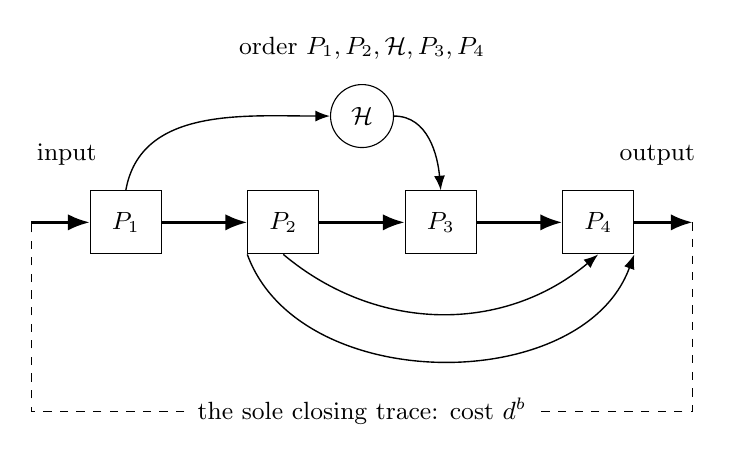
\begin{tikzpicture}[
  >=Latex,
  primary/.style={draw,rectangle,minimum width=9mm,minimum height=8mm},
  hessian/.style={draw,circle,minimum size=8mm},
  bundle/.style={->,line width=1.1pt},
  index/.style={->,line width=.5pt},
  font=\small]
 \node[primary] (p1) at (0,0) {$P_1$};
 \node[primary] (p2) at (2,0) {$P_2$};
 \node[hessian] (h) at (3,1.35) {$\mathcal H$};
 \node[primary] (p3) at (4,0) {$P_3$};
 \node[primary] (p4) at (6,0) {$P_4$};
 \coordinate (in) at (-1.2,0);
 \coordinate (out) at (7.2,0);
 \draw[bundle] (in) -- (p1);
 \draw[bundle] (p1) -- (p2);
 \draw[bundle] (p2) -- (p3);
 \draw[bundle] (p3) -- (p4);
 \draw[bundle] (p4) -- (out);
 \draw[index] (p1.north) to[out=80,in=180] (h.west);
 \draw[index] (h.east) to[out=0,in=95] (p3.north);
 \draw[index] (p2.south) to[out=-40,in=-140] (p4.south);
 \draw[index] (p2.south west) to[out=-70,in=-110] (p4.south east);
 \draw[dashed] (out) -- (7.2,-2.4) -- (-1.2,-2.4) -- (in);
 \node[fill=white,inner sep=3pt] at (3,-2.4)
   {the sole closing trace: cost $d^b$};
 \node[anchor=south] at (3,1.95)
   {order $P_1,P_2,\mathcal H,P_3,P_4$};
 \node[anchor=south] at (-.75,.60) {input};
 \node[anchor=south] at (6.75,.60) {output};
\end{tikzpicture}

\caption{A schematic term with four primary tensors
$P_i=\nabla^{j+e_i}V$ after removing the adjoint divergences.  Thick arrows are the surviving trace-chain
bundles; thin arrows are new contracted indices.  Here
$\mathcal H=\nabla^2H_\rho$ is the Hessian factor, inserted
between its first and last primary neighbors.  The arrows specify matrix inputs and outputs, so every factor
acts across a nontrivial split.  The dashed closure is the one trace
in \eqref{eq:divergence-single-trace}; its cost $d^b$ becomes bounded
after taking a sufficiently high moment root.}
\label{fig:tensor-cut}
\end{figure}

\paragraph{Uniform high-moment bookkeeping.}
The coordinate expansion and its contraction estimate are now complete.
It remains to verify that their constants allow $s$ to grow with $d$
and $j$.  Apply the induction hypothesis to every primary factor with
moment exponent $2s$, and use the pointwise Hessian estimates on all
other factors.  There are exactly $2s$ random primary factors, so H\"older's
inequality uses no larger exponent.  The power of $1/\sqrt a$ before
taking the $2s$-th root is at most
\[
 2s(k_V+j)+\sum_i e_i+\sum_v h_v
 \le 2s(k_V+j+1).
\]
Since $e_i,h_v\le2s$, all polynomial bases in the inductive estimates
are at most $C(s+j+\log(d+1))$.  The total exponent of those bases is
at most
\[
 C\left(2s(j+1)+\sum_i e_i+\sum_v(h_v+1)\right)
 \le C's(j+1),
\]
using \eqref{eq:network-degree-count}.  The term count $(Cs)^{Cs}$
is absorbed in the same bound.  The cut bundle uses only the original free slots of
$T=\nabla^*(\nabla^jV)$, not the new indices introduced by
integration by parts.  Consequently $b\le j+C_V$, where $C_V$
depends only on the fixed number of slots of $V$, and not on $s$.  We have proved
\[
 \E\|T\|_{\op}^{2s}
 \le d^{j+C_V}
       [C(s+j+\log(d+1))]^{Cs(j+1)}
       (\sqrt a)^{-2s(k_V+j+1)}.
\]
Choose $s$ to be the smallest positive integer satisfying $2s\ge p$
and $s\ge(j+C_V)\log(d+1)$, increasing $C_V$ if necessary.
Then $d^{(j+C_V)/(2s)}\le e^{1/2}$ and
\[
 s\le C_V\bigl(p+(j+1)\log(d+1)\bigr).
\]
The expression on the right is bounded by a fixed multiple of
$(p+j+\log(d+1))^2$.  Taking the $2s$-th root, using monotonicity
of probability-space $L^p$ norms, and increasing $C_E$ now gives
\eqref{eq:network} with $k=k_V+1$.

All integration-by-parts identities above are legitimate for each
finite $j,s,d$ and each $\rho<1$.  Indeed, the conditional-integral
regularity in Proposition~\ref{prop:gaussian-jets}, together with
the score formula, gives polynomial growth for every field and
derivative appearing in the finite expansion.  The laws $\xi_\rho$
have Gaussian tails.  Cutoffs therefore justify the identities with
vanishing boundary terms.  Uniformity in growing $s$ is supplied by
the explicit estimates after the identities, not by an unproved
uniform regularity assertion.  This completes the induction.
\end{proof}

\Needspace{9\baselineskip}
\subsection{One final vector dimension factor}

The preceding theorem controls every tensor expression while at least
two slots remain.  Only the last divergence producing a vector will
cost a $\sqrt d$ factor.  The following elementary identity makes
that cost explicit.

\begin{lemma}[Frobenius divergence estimate]
\label{lem:divergence-l2}
Let $\mu(dy)\propto e^{-H(y)}dy$, where $H\in C^2(\R^d)$
has bounded Hessian and $\mu$ has Gaussian tails.  Let $V$ be a smooth
tensor field with a distinguished divergence slot and with
$V,\nabla V\in L^2(\mu)$ in Frobenius norm.  Then
\begin{equation}
 \|\nabla^*V\|_{F,2}
 \le C\bigl(\|V\|_{F,2}+\|\nabla V\|_{F,2}\bigr),
 \label{eq:divergence-l2}
\end{equation}
where $C$ depends only on $\|\nabla^2H\|_{\op,\infty}$, and is
independent of $d$ and the number of remaining tensor slots.
For $H=H_\rho$ it is an absolute constant.
\end{lemma}

\begin{proof}
First take a compactly supported smooth vector field, so that the
output is scalar.  Integrating by parts twice gives
\[
 \int(\nabla^*V)^2\,d\mu
 =\int\sum_{i,j}
     \left[(\partial_iV_j)(\partial_jV_i)
                  +V_i(\partial_{ij}H)V_j\right]d\mu.
\]
The first term is bounded in absolute value by $|\nabla V|_F^2$,
and the second by $\|\nabla^2H\|_{\op}|V|^2$.  For tensor output,
apply the scalar identity to each fixed collection of remaining
indices and sum.  Taking a square root proves
\eqref{eq:divergence-l2} for compactly supported fields.  For general
$V$, multiply by smooth cutoffs $\chi_R$ equal to one on the ball of
radius $R$, with $|\nabla\chi_R|\le C/R$.  Then $\chi_RV\to V$
and $\nabla(\chi_RV)\to\nabla V$ in $L^2(\mu)$, while their
adjoint divergences converge pointwise.  Fatou's lemma proves the
stated estimate.  All fields to which we apply it have polynomially
growing derivatives and hence satisfy the required integrability.
\end{proof}

\begin{corollary}[Derivatives along transported paths]
\label{cor:path-derivatives}
For each fixed integer $m\ge1$,
\begin{equation}
 \|\mathcal D^mM_\rho\|_{L^2(\xi_\rho)}
 \le\polylog(d)L\sqrt d\,a^{-m}.
 \label{eq:path-mean}
\end{equation}
For fixed integers $q\ge1$, $m\ge0$, and fixed real
$2\le p<\infty$, every nontrivial split satisfies
\begin{equation}
 \bigl\|\,|\mathcal D^mU_q|_{\mathrm{split}}\,\bigr\|_{L^p(\xi_\rho)}
 \le\polylog(d)L(\sqrt a)^{-(q-1+2m)}.
 \label{eq:path-jet}
\end{equation}
The constants hidden in $\polylog(d)$ may depend on $m,q,p$
when these parameters occur, but are uniform in $\rho$, the primitive
center, scale, and oracle.
\end{corollary}

\begin{proof}
Iterate Lemma~\ref{lem:material-identities}, using the product rule
on contractions.  Replacing $U_q$ by $\nabla^*U_{q+1}$ raises weight
by two.  Replacing it by one of the contracted products in
\eqref{eq:material-jet-identity} does not raise weight: the two jet
weights sum to $q-1$.  The commutator
\eqref{eq:material-adjoint-identity} inserts $DM_\rho=\rho U_1$
of weight zero on the divergence slot.  Every additional jet factor
$L$ is accompanied by a factor $r$, so, after retaining one overall
$L$, the extra factors are powers of $l=rL\le1$.  Scalar
coefficients are fixed polynomials in $\rho$ and remain bounded
under the fixed number of differentiations.  Starting from a jet
$U_q$, all divergences retain at least two free slots, and all
contractions retain a slot of each factor.  The resulting terms are
therefore expressions of Theorem~\ref{thm:tensor-divergence}, of weight
at most $q-1+2m$.  Its case $j=0$ proves \eqref{eq:path-jet}.

Starting instead from $M$, the first identity is
$\mathcal DM=\nabla^*U_1$.  Its outermost divergence remains a
divergence to a vector under further material differentiations.
Inside it, the same construction gives finitely many normalized
expressions of weight at most $2(m-1)$, each with one overall factor
$L$.  Apply Lemma~\ref{lem:divergence-l2} at this outermost operation.
For a tensor with at least two slots, its Frobenius norm is at most
$\sqrt d$ times the operator norm of an unfolding that puts one
coordinate slot on one side: that matrix has at most $d$ singular
values.  Thus Theorem~\ref{thm:tensor-divergence}, for $j=0,1$ and
$p=2$, bounds the right side of \eqref{eq:divergence-l2} by
\[
 \polylog(d)L\sqrt d\,(\sqrt a)^{-(2m-1)}
 \le\polylog(d)L\sqrt d\,a^{-m}.
\]
This is \eqref{eq:path-mean}.
\end{proof}

To see the quantitative connection with quadrature, start the transport
at its correct marginal and put $Q_\rho=M_\rho(Y_\rho)$.
Proposition~\ref{prop:transport} ensures that $Y_\rho\sim\xi_\rho$,
so \eqref{eq:path-mean} bounds $\|Q_\rho^{(m)}\|_2$ for every
probability time.  On a cell $[\rho_0,\rho_1]\subset[0,1)$ of length
$h_c$, Taylor's integral remainder and the $L^2$ triangle inequality give,
for every $\rho\in[\rho_0,\rho_1]$,
\[
 \left\|Q_\rho-
       \sum_{h=0}^{m-1}\frac{(\rho-\rho_0)^h}{h!}Q_{\rho_0}^{(h)}\right\|_2
 \le \frac{h_c^m}{m!}\sup_{t\in[\rho_0,\rho_1]}\|Q_t^{(m)}\|_2
 \le C_m\polylog(d)L\sqrt d\,
             h_c^m(1-\rho_1^2)^{-m}.
\]
In particular, for a mesh ratio $\theta>0$, the condition
$h_c\le\theta(1-\rho_1)$ makes this remainder at most
$C_m\polylog(d)L\sqrt d\,\theta^m$.
This is a supremum of deterministic RMS bounds; it does not require
an expected supremum over a random trajectory.  The proof of
Proposition~\ref{prop:probability-circuit} uses this cancellation
between cell length and endpoint singularity in polynomial quadrature.
Before constructing those finite formulas, we use the material identity
itself to produce a stationary flow whose path integral represents a
noisy mean.

\section{A stationary flow for noisy means}\label{sec:centering}

The probability transport turns conditional means into samples.  We now
construct the complementary operation: a path integral whose law is
$N(u,s^2I_d)$ for a prescribed $s>0$.  The key is to represent the centered
observable $M_*-u$ as a matrix adjoint divergence.  That matrix couples a
position with law $\xi_*$ to a Gaussian momentum while preserving their
product law; integrating the momentum equation then produces the noisy
mean.  This is still an exact mathematical construction: both its velocity
and its ideal initial law will need to be implemented later.

Retain the primitive and interpolation notation of
Sections~\ref{sec:preliminaries}--\ref{sec:divergence}.  Thus
$L=\lambda r$, $l=\lambda r^2\le1/2$, $M_0=u$, and the symmetric first
jet satisfies $DM_\rho=\rho U_1$.  Fix
\[
 0<R<1/2,\qquad b_*=(1-R^2)^{1/2},
\]
and use a star for evaluation at $\rho=b_*$.  The positive smoothing
radius $R$ keeps all coefficients smooth, although $F$ itself is only
$C^2$.  In this section $\rho$ is the Gaussian-interpolation parameter;
the new stationary flow will use a separate time variable $t$.

\subsection{Transport Jacobians and the zero endpoint}

Let $T_\rho=T_{\rho\to b_*}$ denote the probability transport
\eqref{eq:transport} from time $\rho$ to time $b_*$.  Given a terminal
position $y$, define
\[
 Y_\rho(y)=T_\rho^{-1}(y),\qquad
 B_\rho(y)=DT_\rho(Y_\rho(y))=(DY_\rho(y))^{-1}.
\]
In particular, $Y_{b_*}(y)=y$.  The backward path satisfies
$Y_\rho'=-rM_\rho(Y_\rho)$ with this terminal condition.  Its spatial
Jacobian $J_\rho=DY_\rho$ solves
\[
 J_\rho'=-rDM_\rho(Y_\rho)J_\rho,\qquad J_{b_*}=I_d.
\]
Differentiating its inverse gives the order of multiplication in
\begin{equation}\label{eq:backward-jacobian}
 B_\rho'=rB_\rho DM_\rho(Y_\rho)
         =r\rho B_\rho U_1(\rho,Y_\rho),\qquad B_0'=0.
\end{equation}
The last equality is an exact endpoint identity, not an asymptotic
estimate.  Also $\|B_\rho\|_{\op}\le C$, because
$r\|DM_\rho\|_{\op}\le Cl$ and the time interval has length at most
one.  The following estimates control both spatial differentiation of
the kernel and time interpolation of $B_\rho$.

\begin{lemma}[Transport derivatives]\label{lem:transport-derivatives}
For each fixed $k\ge1$, the order-$k$ spatial derivatives of any transport
between two times in $[0,b_*]$, after subtracting the identity map, have
all nontrivial split norms at most
\[
 C_k lR^{-(k-1)}.
\]
For each fixed $m\ge1$ and fixed finite $p\ge1$, uniformly in
$0\le\rho\le b_*$,
\[
 \big\|\|B_\rho^{(m)}(y)\|_{\op}\big\|_{L^p(y\sim\xi_*)}
 \le \polylog(d)\,l(1-\rho^2)^{-m}.
\]
The constants and the polylogarithmic factor may depend on the fixed
orders and on $p$, but not on the primitive center or scale.
\end{lemma}

\begin{proof}
Differentiate the transport equation with respect to its starting
position.  Gronwall's inequality gives a bounded first derivative and an
$O(l)$ bound for its difference from $I_d$.  For order $k>1$, the chain
rule has terms consisting of an order-$j$ derivative of the velocity
and derivatives of the state of orders $i_1,\ldots,i_j\ge1$, where
$i_1+\cdots+i_j=k$.  By \eqref{eq:jets}, the outer tensor has every
split norm at most $C_j lR^{-(j-1)}$.  Attach the inner tensors one at
a time.  Each attachment is a single contraction retaining the outer
output and the inner derivative slots, so
Lemma~\ref{lem:split-contraction} applies without a dimension factor.
Bound a first state derivative by a constant and use the induction
hypothesis for all higher state derivatives.  Since $l\le1$, the total
power of $R^{-1}$ is at most
\[
 (j-1)+\sum_{\nu=1}^j(i_\nu-1)=k-1,
\]
and each forcing term retains the outer factor $l$.  The term involving
the unknown order-$k$ state derivative is linear, with coefficient
bounded by $Cl$, and this derivative starts at zero.  Gronwall proves
the assertion.  The same argument with absolute interval lengths
applies to transport in the reverse direction.

For the second assertion, write
$C_\rho=rDM_\rho(Y_\rho)=r\rho U_1(\rho,Y_\rho)$, so that
$B_\rho'=B_\rho C_\rho$.  The product rule expresses $B_\rho^{(m)}$
as a finite sum of ordered products of $B_\rho$ and $k\ge1$ factors
$C_\rho^{(j_1)},\ldots,C_\rho^{(j_k)}$, with
$j_1+\cdots+j_k=m-k$.  The zero-order jet bound and
\eqref{eq:path-jet} imply, for every fixed moment order,
\[
 \big\|\|C_\rho^{(j)}\|_{\op}\big\|_{L^p}
 \le \polylog(d)\,l(1-\rho^2)^{-j}.
\]
Here the path estimates apply because inverse transport sends
$y\sim\xi_*$ to $Y_\rho(y)\sim\xi_\rho$.  Apply H\"older with
sufficiently high fixed moments to each product.  Using $l^k\le l$
and $(1-\rho^2)^{-(m-k)}\le(1-\rho^2)^{-m}$ gives the claimed
conservative exponent.  Moments below one, if desired, follow from
the $L^1$ bound.
\end{proof}

\subsection{A kernel for the centered observable}

For a matrix field $K$, define its row-wise adjoint divergence by
\[
 (\nabla_{\xi_*}^*K)_i
 =\sum_j\{-\partial_jK_{ij}+(\partial_jH_*)K_{ij}\}.
\]
Thus $\nabla_{\xi_*}^*K=h$ means
$\E_{\xi_*}[h_i\phi]=\E_{\xi_*}\sum_jK_{ij}\partial_j\phi$
for smooth compactly supported scalar tests $\phi$.  We seek this
identity with $h=M_*-u$.

This is a Stein-type integration-by-parts identity.  A classical
coordinate Stein kernel for a law $\xi$ represents the observable
$y-\E_\xi y$ instead.  Courtade, Fathi and Pananjady construct such
kernels from spectral-gap assumptions
\citep[arXiv version~2, Definition~2.1 and Theorem~2.4]{courtade2019stein}.
Our observable is $M_*-u$; its mean is zero by conditional expectation.
The transport formula below supplies its particular adjoint-divergence
representation together with pointwise derivative bounds.  Those bounds
are needed for quadrature and do not follow from the cited existence
statement.  We do not require $K$ to be symmetric or positive.

Define
\begin{equation}\label{eq:stein-kernel}
 K(y)^T=\int_0^{b_*}B_\rho(y)U_1(\rho,Y_\rho(y))\,d\rho
       =\frac1r\int_0^{b_*}B_\rho'(y)\,\frac{d\rho}{\rho}.
\end{equation}
The first integral defines the integrand at zero in the second formula:
$B_\rho'/(r\rho)=B_\rho U_1(\rho,Y_\rho)$ extends smoothly there.
The transpose is essential: the adjoint divergence will act on the
rows of $K$, while the position velocity will use $K^T$.

\begin{lemma}[The centering kernel]\label{lem:centering-kernel}
The field $K$ is smooth and satisfies
\[
 \nabla_{\xi_*}^*K=M_*-u,\qquad \|K(y)\|_{\op}\le CL.
\]
For each fixed $j\ge1$, every nontrivial split norm of $\nabla^jK$ is
bounded pointwise by $C_jLR^{-j}$.
\end{lemma}

\begin{proof}
Fix an output coordinate $i$ and a smooth compactly supported scalar
function $\phi$.  The transported test $\phi\circ T_\rho$ has zero
material derivative: it is constant along each probability-transport
path.  Differentiate its product with $M_{\rho,i}$ under the
transported laws.  Lemma~\ref{lem:material-identities} gives
$\mathcal DM_\rho=\nabla_{\xi_\rho}^*U_1$, so integration by parts
and the chain rule yield
\[
 \frac{d}{d\rho}\E_{\xi_\rho}[M_{\rho,i}\,\phi\circ T_\rho]
 =\E_{\xi_\rho}\sum_{j,k}(U_1)_{ik}(DT_\rho)_{jk}
                                  (\partial_j\phi)\circ T_\rho.
\]
Smooth transport on the compact time interval and Gaussian tails
justify differentiation; alternatively the test can first be cut off
and the resulting identities passed to the limit.  Push the expectation
forward to $y\sim\xi_*$.  Since $U_1$ is symmetric, its coefficient of
$\partial_j\phi(y)$ is
\[
 \sum_k (U_1)_{ik}(\rho,Y_\rho(y))(B_\rho(y))_{jk}
       =(B_\rho(y)U_1(\rho,Y_\rho(y)))_{ji}.
\]
The terminal expectation is $\E_{\xi_*}[M_{*,i}\phi]$.
At zero, $M_0=u$ and $(T_0)_\#\xi_0=\xi_*$, so the initial
expectation is $u_i\E_{\xi_*}\phi$.  Integrating the displayed
derivative in $\rho$ proves
\[
 \E_{\xi_*}[(M_{*,i}-u_i)\phi]
   =\E_{\xi_*}\sum_jK_{ij}\partial_j\phi.
\]
This proves the adjoint-divergence identity weakly, and smoothness
makes it a pointwise identity.

For the bounds, $\|B_\rho\|_{\op}\le C$ and
$\|U_1\|_{\op}\le CL$ immediately give $\|K\|_{\op}\le CL$.
For a positive-order spatial derivative, use
Lemma~\ref{lem:transport-derivatives} on both $DT_\rho$ and
$Y_\rho$.  An order-$j$ derivative of $DT_\rho$ has all split norms
at most $C_jlR^{-j}$, and an order-$j$ derivative of $U_1$ has all
split norms at most $C_jLR^{-j}$ by \eqref{eq:jets}.  When these
fields are composed with $Y_\rho$, attach each chain-rule tensor by
a single edge as in the preceding lemma.  First derivatives of
$Y_\rho$ are bounded, and a derivative of order $i>1$ costs
$C_i lR^{-(i-1)}$.  Every order-$j$ term in the product has total
cost at most $C_jLR^{-j}$, since $l\le1$.  Each factor retains free
slots, so the single-contraction bound preserves every nontrivial
split.  Integrating over an interval of length at most one proves
the assertion.  All orders are smooth by Gaussian conditional
integration and the smooth transport on $\rho\le b_*<1$; this uses
no higher derivatives of the original unsmoothed gradient.
\end{proof}

\subsection{Stationarity and the path integral}

The following dynamics specialize the skew-matrix construction of
Ma, Chen and Fox
\citep[Section~2.1, Equation~(3), Theorem~1]{ma2015recipe}.
The transport-derived $K$ makes the momentum displacement encode
$M_*-u$.  We prove completeness and invariance directly, since a
formal stationary-density calculation alone would not ensure a
solution exists for the full integration interval.

\begin{proposition}[A noisy mean from a path integral]
\label{prop:centering-law}
For $s>0$, let $(Y_0,G_0)$ have law $\xi_*\otimes N(0,I_d)$ and solve
\begin{equation}\label{eq:centering-flow}
 \dot Y_t=-K(Y_t)^TG_t/s,\qquad
 \dot G_t=(M_*(Y_t)-u)/s.
\end{equation}
The solution exists for every finite time, and its law remains
$\xi_*\otimes N(0,I_d)$.  In particular,
\begin{equation}\label{eq:centering-output}
 sG_0+\int_0^1M_*(Y_t)\,dt\ \stackrel{\mathrm{law}}=
 u+sG,\qquad G\sim N(0,I_d).
\end{equation}
\end{proposition}

\begin{proof}
The vector field $v$ in \eqref{eq:centering-flow} is smooth and hence
locally Lipschitz.  The bound on $K$ and the global Lipschitz bound on
$M_*$ imply $|v(y,g)|\le C_{x,r,s}(1+|y|+|g|)$.  Gronwall's
inequality therefore prevents a solution from escaping to infinity
in finite positive or negative time.  Local uniqueness gives a
complete smooth flow $\Phi_t$, with inverse $\Phi_{-t}$.  We only
need local Lipschitz continuity here; the factor $G$ does not in
general give a globally Lipschitz joint vector field.

Write the product density as
\[
 p(y,g)=(2\pi)^{-d/2}\exp(-H_*(y)-|g|^2/2).
\]
Differentiating in the position and momentum variables separately,
with the row convention of the kernel lemma, gives
\[
 \operatorname{div}_y(pv_Y)
   =\frac{p}{s}\sum_i g_i(\nabla_{\xi_*}^*K)_i
   =\frac{p}{s}\,g\cdot(M_*-u),\qquad
 \operatorname{div}_g(pv_G)
   =-\frac{p}{s}\,g\cdot(M_*-u).
\]
Thus $\operatorname{div}(pv)=0$.  The Jacobian formula for the
complete flow now yields, pointwise,
\[
 \frac{d}{dt}\{p(\Phi_t(z))\det D\Phi_t(z)\}
   =\operatorname{div}(pv)(\Phi_t(z))\det D\Phi_t(z)=0.
\]
The determinant starts at one and stays positive.  Change of variables
therefore proves that $\Phi_t$ preserves the probability density $p$.

For later differentiation it is useful to record the same cancellation
as an operator identity.  Relative to the product law, the Lie
derivative is
\begin{equation}\label{eq:centering-skew-operator}
 \mathcal L=\nabla^*A\nabla,\qquad
 A=\begin{pmatrix}0&K^T/s\\-K/s&0\end{pmatrix}.
\end{equation}
Indeed the second-order part vanishes by skew symmetry.  The
first-order coefficients are $-K^Tg/s$ in position and
$\nabla_{\xi_*}^*K/s=(M_*-u)/s$ in momentum, exactly as in
\eqref{eq:centering-flow}.

Finally, integrating the momentum equation over $[0,1]$ gives the
pathwise identity
\[
 sG_0+\int_0^1M_*(Y_t)\,dt=u+sG_1.
\]
Stationarity makes $G_1$ a standard Gaussian, proving
\eqref{eq:centering-output}.
\end{proof}

Stationarity also makes $G_1$ independent of $Y_1$.  It does not assert
that $G_1$ is independent of the initial anchors $(Y_0,G_0)$.
The exact mean $u=M_0$ remains in the momentum velocity, and the
proposition assumes an ideal sample from $\xi_*$.  Thus the proposition
is a comparison construction, not yet an oracle routine.  Section~\ref{sec:numerics}
will express its approximation by finitely many exact mean evaluations;
Section~\ref{sec:compiler} will replace every such evaluation, including
$M_0$.  The displayed output itself needs no separate addition of $u$.

\subsection{Derivatives on a stationary trajectory}

To approximate the path integral by high-order quadrature, we need
bounds on time derivatives at each fixed time.  Stationarity allows
these bounds to be proved in the fixed product measure.  The following
lemma separates that argument from the particular kernel and avoids
requiring a bound on the supremum of a random path.

\begin{lemma}[Stationary time derivatives]\label{lem:stationary-derivatives}
Fix $0<R\le1$.  Let a smooth probability density on $\R^n$, with
$n\le Cd$, have Gaussian tails and negative logarithm $H$.  Assume
its Hessian is bounded and that every positive-order score derivative
$\nabla^j\nabla H$ has every one-slot split norm at most
$C_jR^{-(j-1)}$, for $j\ge1$.  Here a one-slot split isolates one
tensor slot as the matrix input and groups all remaining slots as
its output.  Suppose a stationary autonomous flow has Lie derivative
$\mathcal L=\nabla^*A\nabla$, where the adjoint is for this density,
$A$ is skew symmetric, and
\[
 |\nabla^jA|_{\text{one-slot split}}\le C_j\alpha R^{-j}
 \quad(j\ge0)
\]
for every one-slot split.  Let $\phi_0$ be smooth and scalar- or
vector-valued, with
\[
 |\nabla^j\phi_0|_F\le C_ja_0\sqrt d\,R^{-j}
 \quad(j\ge1).
\]
Assume the fields and all derivatives used have polynomial growth.
Then, for each fixed $k\ge1$, the order-$k$ time derivative of
$\phi_0$ on the stationary flow has RMS norm at most
\begin{equation}\label{eq:stationary-derivatives}
 C_k a_0\sqrt d\,(\alpha R^{-2})^k.
\end{equation}
\end{lemma}

\begin{proof}
Put $\phi_k=\mathcal L^k\phi_0$.  We prove, for $j\ge0$ and
$k\ge1$, the stronger estimate
\begin{equation}\label{eq:stationary-spatial-induction}
 \|\nabla^j\phi_k\|_{F,2}
 \le C_{j,k}a_0\sqrt d\,\alpha^kR^{-(j+2k)}.
\end{equation}
For $k=0$ the same bound is assumed only for $j\ge1$, which suffices:
the iteration differentiates $\phi_{k-1}$ before multiplying by $A$.
All $L^2$ norms below are for the invariant density.

Set $V=A\nabla\phi_{k-1}$.  Leibniz's rule and the induction
hypothesis give, for each $h\ge0$,
\[
 \|\nabla^h V\|_{F,2}
 \le C_{h,k}a_0\sqrt d\,\alpha^k
                         R^{-(h+1+2(k-1))}.
\]
To see why no dimension factor appears, in each coefficient tensor
$\nabla^vA$ isolate the slot contracted against the gradient of
$\phi_{k-1}$.  Its one-slot operator norm multiplies the Frobenius
norm of the other factor.  Summing the finitely many Leibniz terms
preserves the displayed estimate.

Now commute $j$ derivatives past the adjoint divergence in
$\phi_k=\nabla^*V$.  The main term is $\nabla^*(\nabla^jV)$.
The Frobenius estimate \eqref{eq:divergence-l2} bounds its $L^2$ norm
by a constant times
$\|\nabla^jV\|_{F,2}+\|\nabla^{j+1}V\|_{F,2}$.
These two terms have powers $R^{-(j+2k-1)}$ and
$R^{-(j+2k)}$, respectively.  Each remaining commutator contracts
an order-$v$ derivative of the score, $1\le v\le j$, with
$\nabla^{j-v}V$.  The coefficient's one-slot norm again suffices;
the total exponent of $R^{-1}$ is
\[
 (v-1)+(j-v+1+2(k-1))=j+2k-2.
\]
All these terms are bounded by
\eqref{eq:stationary-spatial-induction} because $0<R\le1$.
This closes the induction, including $j=0$ for $k\ge1$.
Gaussian tails and polynomial growth justify the integrations by
parts through cutoffs.

Along an autonomous trajectory, the $k$th time derivative of
$\phi_0$ is $\phi_k$ evaluated at the current state.  Stationarity
identifies its RMS norm at every time with the fixed-measure norm
in \eqref{eq:stationary-spatial-induction} for $j=0$.
\end{proof}

For \eqref{eq:centering-flow}, the ambient dimension is $2d$, and
\eqref{eq:centering-skew-operator} satisfies the lemma's coefficient
bounds with $\alpha=L/s$.  The product potential is
$H_*(y)+|g|^2/2$; its score-derivative bounds follow from
\eqref{eq:jets} and the Gaussian factor.  For the joint state take
$a_0=1$: its first derivative has Frobenius norm $\sqrt{2d}$ and
all higher derivatives vanish.  For $M_*$ take $a_0=L$.
Indeed, isolating any derivative slot in \eqref{eq:jets} gives a
matrix with input dimension $d$, so passage from its operator norm
to its Frobenius norm costs at most $\sqrt d$.
Consequently, at every stationary time,
\[
 \left\|\frac{d^k}{dt^k}(Y_t,G_t)\right\|_2
       \le C_k\sqrt d\,((L/s)R^{-2})^k,\qquad
 \left\|\frac{d^k}{dt^k}M_*(Y_t)\right\|_2
       \le C_kL\sqrt d\,((L/s)R^{-2})^k.
\]
The strict radius choice $0<R<1/2$ made for this construction
satisfies the abstract lemma's $0<R\le1$ hypothesis.

We also need an initial displacement estimate for the later iteration.
Conditional expectation and the primitive Poincar\'e inequality give
\[
 \E_{\xi_*}|M_*-u|^2
 \le\E_\nu|f-u|^2\le CL^2d.
\]
At every stationary time, $G_t$ is independent of $Y_t$, hence
\[
 \E|K(Y_t)^TG_t|^2
   =\E\|K(Y_t)\|_F^2\le CL^2d.
\]
Integrate the velocity and apply Minkowski's inequality to obtain
\begin{equation}\label{eq:centering-initial-displacement}
 \|(Y_t,G_t)-(Y_0,G_0)\|_2
 \le Ct(L/s)\sqrt d\le C(L/s)\sqrt d
 \qquad(0\le t\le1).
\end{equation}
These are fixed-time RMS estimates for the exact stationary flow.
They give the derivative and starting-error bounds used in the next
section to approximate its path integral by finite formulas.

\section{Finite formulas for the two flows}\label{sec:numerics}

We now turn the probability transport and the stationary centering flow
into finite formulas in conditional means.  The formulas must meet two
requirements at once.  Their error on the prescribed input law must be
small, and each new mean must be evaluated at a center that is an affine
expression in earlier mean values, with scalar coefficients and controlled
size.  The latter property permits the recursive implementation in the
next section.

The main conclusion is Theorem~\ref{thm:numerical-interface}.  Its proof
has three numerical steps.  Global Picard iteration discretizes
probability transport without making the dependency depth proportional
to the number of time cells.  Short harmonic trajectories then give a
formula for the vector $K(y)^TG$ in the centering velocity.  Finally,
Picard iteration discretizes that stationary flow.  Two cancellations
are needed in the middle step: a zero derivative removes the singularity
at the lower endpoint of the kernel integral, and retaining only a
forward transport \emph{correction} cancels its apparent inverse power
of the primitive scale $r$.

Polynomial collocation of Picard iteration was developed for sampling
by \citet[Algorithm~2 and Theorem~2.3]{lee2018odes}; Gaussian smoothing
and high-order Picard approximation also appear in
\citet[Appendix~E, Algorithm~E.1 and Theorem~E.2]{chen2026picard}.
Here we need, in addition, scalar affine formulas whose dependency depth
can be fixed before their interpolation order.  An exact conditional
mean is an analytical node throughout this section.  The next section
replaces these nodes by finite oracle computations.

Fix an integer $K_0\ge2$ and $t>0$ such that
\begin{equation}\label{eq:numerical-parameters}
 40(K_0+2)t<\frac14,\qquad
 R=\delta^t,\qquad \psi=\delta^{4t},\qquad h_0=\delta^w,\qquad 0<w<t.
\end{equation}
The iteration count will first fix a depth bound.  We then choose $w$
and finally the interpolation orders; increasing those orders will not
change the depth bound.  For the centering flow set $s=\sigma/2$, where
$\sigma>0$ is the parent mean-noise parameter.  Thus the centering
formula itself will approximate noise of standard deviation $\sigma/2$.
Throughout its numerical analysis assume
\begin{equation}\label{eq:numerical-size}
 \max\{l,L/\sigma\}\le\polylog(d)\delta^b,\qquad b\ge\frac12.
\end{equation}
For probability transport alone only the corresponding bound on $l$ is
required.  All probability-time intervals lie in
$[0,(1-cR^2)^{1/2}]$, for a fixed $c>0$.  Constants may depend on fixed
interpolation orders and fixed parameters, but not on the center,
dimension, primitive scale $r$, noise parameter, or oracle.  A symbol
$B_d$ below denotes a bound $C(1+\log d)^C$ with precisely this uniformity;
the fixed exponent and constant in a size hypothesis are part of the
fixed parameters.  All assertions are for sufficiently large $d$.

\subsection{Probability transport by global Picard iteration}

Partition a probability-time interval using equal steps of size at most
$h_0$ in $-\log(1-\rho)$.  For a nonzero interval take the ceiling of
its transformed length divided by $h_0$ as the number of cells.
Cell lengths $\ell_c$ then obey
$\ell_c\le C h_0(1-\rho)$ on that cell, and the number of cells is
\[
 O\bigl(1+h_0^{-1}(1+|\log R|)\bigr).
\]
A zero-length interval requires no operations.  On each cell interpolate
at $m\ge2$ distinct equally spaced nodes, including both ends, and
integrate the resulting degree-$(m-1)$ polynomial.  Include partial
integrals to every state node.  By scaling the fixed Lagrange basis on
$[0,1]$, its absolute value sum is at most $C_m$, and its order-$k$
derivative absolute sum is at most $C_m\ell_c^{-k}$.
Consequently every partial-integral row has absolute weight sum at most
$C_m$, uniformly in the number of cells.

Let $w_{ij}$ be these partial-integral weights from the starting time
$\rho_{\mathrm{in}}$ to node $\rho_i$, with signed weights for backward
integration.  Duplicate shared endpoints as labeled nodes if convenient.
Given a starting position $y_{\mathrm{in}}$, use simultaneous updates
\begin{equation}\label{eq:probability-update}
 y_i^{[0]}=y_{\mathrm{in}},\qquad
 y_i^{[k+1]}=y_{\mathrm{in}}-
 r\sum_j w_{ij}M_{\rho_j}(y_j^{[k]}).
\end{equation}
This iteration integrates over the whole interval at every layer; it does
not advance successively from cell to cell.

\begin{proposition}[Probability-flow circuit]
\label{prop:probability-circuit}
If the input position has marginal law $\xi_{\rho_{\mathrm{in}}}$, then
after $N_p$ iterations the maximum, over all state nodes, of the RMS
error relative to the exact transport is at most
\begin{equation}\label{eq:probability-picard}
 C_m\polylog(d)\,l\sqrt d\,h_0^m
       +(C_ml)^{N_p}CrD.
\end{equation}
Every computed state is globally Lipschitz in its initial position with
constant $C_m$.  After subtracting the initial position, its Lipschitz
constant is at most $C_ml$.
\end{proposition}

\begin{proof}
Write $Y_\rho$ for the exact path from the given random input and
$Q_\rho=M_\rho(Y_\rho)$.  The marginal identity in
Proposition~\ref{prop:transport} and \eqref{eq:path-mean} give
\[
 \|Q_\rho^{(m)}\|_2\le B_dL\sqrt d(1-\rho^2)^{-m}.
\]
On a cell $I=[a_c,b_c]$ of length $\ell_c$, let $P$ be the
Taylor polynomial of $Q$ of degree $m-1$ at $a_c$.  Minkowski's
inequality applied to the integral remainder gives, at each $v\in I$,
\begin{equation}\label{eq:numerical-taylor-remainder}
 \|Q_v-P(v)\|_2
 \le \frac1{(m-1)!}\int_{a_c}^v
       (v-z)^{m-1}\|Q_z^{(m)}\|_2\,dz
 \le C_mB_dL\sqrt d\,h_0^m.
\end{equation}
The last step uses $\ell_c\le Ch_0(1-z)$ on that cell and
$1-z^2\ge1-z$.  The same estimate holds at the interpolation nodes.
Because interpolation reproduces $P$ and its basis has bounded absolute
sum, $\|Q_v-\mathcal I_cQ(v)\|_2$ obeys the same bound.
Integrate this pointwise estimate over the cells, whose total length
is at most one.  This proves the required quadrature error, for partial
integrals and for either orientation.  No supremum of the random path
has been taken.

Let $e_k=\max_i\|y_i^{[k]}-Y_{\rho_i}\|_2$.  The global bound
$\Lip(M_\rho)\le CL$, together with the absolute row sums, gives
\[
 e_{k+1}\le C_ml e_k+C_mB_dl\sqrt d\,h_0^m.
\]
On each exact transported marginal, conditional expectation and the
primitive moment bound give $\|M_\rho\|_2\le CD$.  Integrating the
velocity shows $e_0\le CrD$.  Since $C_ml<1/2$ for large $d$, summing
the geometric recurrence proves \eqref{eq:probability-picard}.
The norm here is the maximum of the nodewise RMS errors; it is not the
RMS of their maximum.

For deterministic inputs the same recurrence, now in maximum node norm,
gives a bounded Lipschitz constant for every iterate.  In the correction
$y_i^{[k+1]}-y_{\mathrm{in}}$, the factor $r$ and the $CL$-Lipschitz mean
give the stronger constant $C_ml$.
\end{proof}

\subsection{The kernel action through harmonic trajectories}

The position velocity in \eqref{eq:centering-flow} contains $K(y)^TG$.
Approximating $K$ and then multiplying the error by an arbitrary momentum
would not give the global Lipschitz property needed for Picard iteration.
Instead we approximate the vector action directly, using short harmonic
trajectories and forward transport corrections.

For the kernel integral use the mesh on $[0,b_*]$ above.  Its cell lengths
also satisfy $\ell_c\ge c'h_0(1-\rho)$ for all sufficiently large $d$;
this follows from the ceiling construction because the transformed
interval length tends to infinity.  Set
$C_\rho(y)=B_\rho(y)-I$.  We first describe a circuit for
$C_\rho(y)G$ at one probability node $\rho$.

\paragraph{Backward position.}
Apply Proposition~\ref{prop:probability-circuit} backward from input
position $y$ at time $b_*$ to obtain an approximation $\widehat Y_\rho$
to $Y_\rho(y)$.

\paragraph{Short harmonic trajectories.}
At fixed probability time $\rho$, the Hamiltonian equations with
potential $H_\rho$ have position integral equation
\begin{equation}\label{eq:harmonic-integral}
 W_z=\cos(z)Y_\rho+\sin(z)G
      -r\rho\int_0^z\sin(z-v)M_\rho(W_v)\,dv.
\end{equation}
For every requested angle $z$, interpolate on the single cell $[0,z]$.
Let $z_i$ be its nodes and $\ell_j(v)$ its Lagrange basis, and set
\[
 w_{ij}^{\sin}=\int_0^{z_i}\sin(z_i-v)\ell_j(v)\,dv.
\]
Use the simultaneous Picard updates
\begin{equation}\label{eq:harmonic-picard}
 \begin{split}
 W_i^{[0]}&=\cos(z_i)\widehat Y_\rho+\sin(z_i)G,\\
 W_i^{[k+1]}&=\cos(z_i)\widehat Y_\rho+\sin(z_i)G
      -r\rho\sum_jw_{ij}^{\sin}M_\rho(W_j^{[k]}).
 \end{split}
\end{equation}
At angle zero there is no integral.  The free sine and cosine terms
are retained exactly.

\paragraph{Differentiate the transport correction.}
Let $d_j$ be the weights differentiating at zero the polynomial
interpolant on angle nodes $0,\psi,\ldots,(m-1)\psi$.  Their absolute
sum is $C_m\psi^{-1}$.  At every such angle node, compute
$T_\rho(W_z)-W_z$ by the forward probability-flow circuit, keeping only
its integral correction at the output.  For exact paths,
\begin{equation}\label{eq:kernel-action-derivative}
 \left.\frac{d}{dz}(T_\rho-\mathrm{id})(W_z)\right|_{z=0}
       =(B_\rho-I)G=C_\rho G,
\end{equation}
since $W_0=Y_\rho$ and $W'_0=G$.  The weighted sum with coefficients
$d_j$ therefore approximates $C_\rho G$ using exact mean nodes only.

Here and below the interpolation orders denoted by $m$ may be increased
independently.  Using a common sufficiently large order merely simplifies
the error displays.  For the next estimates use the same number
$N_p\ge1$ of Picard layers in the backward, harmonic, and forward
computations.

\begin{lemma}[Errors in the angle computation]
\label{lem:kernel-angle-errors}
Let $y\sim\xi_*$ and $G\sim N(0,I_d)$ independently.  The exact-input
angle differentiation in \eqref{eq:kernel-action-derivative} has RMS
truncation error at most
\begin{equation}\label{eq:angle-stencil-error}
 C_m l\sqrt d\,\psi^{m-1}R^{-2m}
       =C_ml\sqrt d\,\delta^{2tm-4t}.
\end{equation}
Before applying the angle differentiation weights, the RMS errors of the
computed forward correction values are at most
\begin{equation}\label{eq:kernel-value-error}
 C_m\polylog(d)\,l\sqrt d\,(h_0^m+\delta^{2tm})
       +(C_ml)^{N_p}CrD.
\end{equation}
Every such approximate correction is globally Lipschitz in $(y,G)$
with constant at most $C_ml$.
\end{lemma}

\begin{proof}
For exact inputs $(Y_\rho(y),G)$, harmonic motion
$\dot W=P$, $\dot P=-\nabla H_\rho(W)$ preserves
$\xi_\rho\otimes N(0,I_d)$.  The vector field is globally Lipschitz,
and its weighted divergence vanishes.  Its Lie derivative is
$\nabla^*A\nabla$ with constant skew coefficient whose $(W,P)$ block
is $-I$.  Lemma~\ref{lem:stationary-derivatives} therefore applies with
$\alpha=1$, with $a_0=l$ for $T_\rho-\mathrm{id}$, and with $a_0=L$
for $M_\rho$.  Indeed Lemma~\ref{lem:transport-derivatives} and
\eqref{eq:jets} give the required spatial bounds; changing a one-slot
split bound to a Frobenius bound costs only $\sqrt d$.
To apply the angle stencil, subtract the Taylor polynomial of
$z\mapsto(T_\rho-\mathrm{id})(W_z)$ of degree $m-1$ at zero.
Its derivative at zero is exact, and its remainder at each stencil
node has RMS norm at most $C_ml\sqrt d\,\psi^mR^{-2m}$.
Multiplication by the absolute stencil sum $C_m/\psi$ proves
\eqref{eq:angle-stencil-error}.  This uses pointwise RMS
remainders on the stationary harmonic path.

For the harmonic state equation, interpolate $M_\rho(W_v)$ in
\eqref{eq:harmonic-integral}.  Since $z\le(m-1)\psi$, its Taylor
remainder, multiplied by the prefactor $r$, is bounded by
$C_ml\sqrt d\,\psi^mR^{-2m}
=C_ml\sqrt d\,\delta^{2tm}$; the additional integration factors are
bounded and can be discarded.  The initial free-path error is at most
$CrD$, and Picard contracts by $C_ml$.  The computed harmonic state is
globally Lipschitz with bounded constant in its two inputs, by the same
row-sum argument as before.

Next compare the forward probability correction started at the exact
harmonic state.  That state has marginal law $\xi_\rho$, so
Proposition~\ref{prop:probability-circuit} applies.  Errors in its
starting state then propagate through the approximate correction with
factor $C_ml$, not a factor of order one.  This also controls the
backward-position error transmitted through the harmonic computation.
Combining these estimates proves \eqref{eq:kernel-value-error} and
the asserted global Lipschitz bound.
\end{proof}

\subsection{The zero endpoint of the kernel integral}

It remains to integrate the derivative of $C_\rho G$ against $1/\rho$.
The exact identity $B'_0=0$ removes the apparent singularity, and we
impose that identity on the interpolant as well.

On all but the first probability cell use ordinary degree-$(m-1)$
interpolation.  On the first cell use $m-1$ equally spaced value nodes
including both endpoints and the additional Hermite condition that the derivative
at zero is zero, for a total of $m$ conditions, with $m\ge3$.
This uniquely determines a polynomial of degree at most $m-1$: a
polynomial in the null space would have a double zero at zero and the
remaining $m-2$ distinct zeros.  Let $q_i$ be the resulting weights on
values when the derivative of this piecewise interpolant is integrated
against $1/\rho$.

\begin{lemma}[Derivative quadrature at zero]
\label{lem:kernel-endpoint-quadrature}
Let $y\sim\xi_*$ and $G\sim N(0,I_d)$ independently.
For exact values of $C_\rho(y)G$, the RMS error of this quadrature for
$\int_0^{b_*}B'_\rho(y)G\,d\rho/\rho$ is at most
\[
 C_m\polylog(d)\,l\sqrt d\,h_0^{m-2}.
\]
The value weights satisfy
\begin{equation}\label{eq:kernel-weight-sum}
 \sum_i|q_i|
 \le C_mh_0^{-1}(1+|\log R|+|\log h_0|).
\end{equation}
These weights are well defined even if the supplied values are
approximate: the derivative condition at zero remains exact.
\end{lemma}

\begin{proof}
By Lemma~\ref{lem:transport-derivatives} and independence of $G$,
the RMS norm of the order-$m$ derivative of $C_\rho(y)G$ is at most
$\polylog(d)l\sqrt d(1-\rho^2)^{-m}$.  Here multiplication by the
independent Gaussian converts the matrix norm to a Frobenius norm and
costs at most $\sqrt d$.

On an ordinary cell, Taylor expansion and scaling the interpolation
basis bound the derivative error by this derivative bound times
$C_m\ell_c^{m-1}$.  It is therefore at most
$C_m\polylog(d)l\sqrt d h_0^{m-1}/(1-\rho)$.
After integration against $1/\rho$, all ordinary cells contribute at
most this prefactor times
$C(1+|\log R|+|\log h_0|)$, which fits the claimed more conservative
$h_0^{m-2}$ bound.

For the first cell, subtract the Taylor polynomial at zero of degree
$m-1$.  Its derivative at zero agrees with the exact zero derivative.
The second derivative of the remainder, and that of the Hermite
interpolant of the remainder, are bounded in RMS by
$C_m\polylog(d)l\sqrt d\,\ell_c^{m-2}$.  Both first derivatives
vanish at zero.  If $E$ is the difference between the exact function
and its Hermite interpolant on this cell, then
\[
 \|E'(\rho)\|_2
 \le\int_0^\rho\|E''(v)\|_2\,dv
 \le C_mB_dl\sqrt d\,\rho\ell_c^{m-2}.
\]
Consequently the integral of $E'(\rho)/\rho$ over the first cell
has RMS norm at most $C_mB_dl\sqrt d\,\ell_c^{m-1}$.
This is within the stated, more conservative $h_0^{m-2}$ bound.

On an ordinary cell the absolute coefficient sum of the interpolant
derivative is at most $C_m/\ell_c$.  Integrating and using
$\ell_c\ge c'h_0(1-\rho)$ gives a total bounded by
\[
 C_mh_0^{-1}\int_{\rho_{\mathrm{first}}}^{b_*}
                   \frac{d\rho}{\rho(1-\rho)}.
\]
This gives the logarithms in \eqref{eq:kernel-weight-sum}.
On the first cell, scale to the unit interval.  The polynomial
derivative vanishes at zero and is bounded by distance to zero times
the second derivative, so the integral of its absolute value divided
by that distance is bounded.  Scaling back gives a weight sum
$C_m/\ell_c\le C_mh_0^{-1}$.  This proves the claim.
\end{proof}

\subsection{A globally Lipschitz approximate centering velocity}

Let $\mathrm{corr}_{ij}(y,G)$ denote the forward correction computed at
probability node $i$ and angle node $j$ by the three operations above.
The approximate position velocity is the explicit expression
\begin{equation}\label{eq:kernel-approximate-velocity}
 \widehat v_Y(y,G)=-\frac1{rs}\sum_iq_i\sum_jd_j
                         \mathrm{corr}_{ij}(y,G).
\end{equation}
Each correction retains only the integral part of the forward Picard
formula. Writing its weights as $w_{ijk}$ and its mean values as
$M_{ijk}$ gives
\[
 \mathrm{corr}_{ij}=-r\sum_kw_{ijk}M_{ijk},
\]
and hence
\begin{equation}\label{eq:kernel-scalar-expansion}
 \widehat v_Y=\frac1s\sum_{i,j,k}q_i d_j w_{ijk}M_{ijk}.
\end{equation}
The apparent factor $1/r$ has canceled algebraically. There is no
additive forward state left in this formula, and all coefficients
multiplying mean values are deterministic scalars.
Use the exact mean expression
$\widehat v_G(y,G)=(M_*(y)-M_0)/s$ for the momentum velocity.
In particular, the momentum occurs inside angle states; it is never
multiplied by a separately approximated matrix at the output.

\begin{proposition}[Kernel-action circuit]\label{prop:kernel-circuit}
On the stationary product input law, the RMS error of
$\widehat v=(\widehat v_Y,\widehat v_G)$ relative to
\eqref{eq:centering-flow} is bounded by $\polylog(d)$ times
\begin{equation}\label{eq:kernel-velocity-error}
 \begin{split}
 &\frac L\sigma\sqrt d
 \left[h_0^{m-2}+h_0^{-1}\delta^{-4t}
                      (h_0^m+\delta^{2tm})\right]\\
 &\hspace{12mm}+\delta^{-4t-w}(C_ml)^{N_p-1}
                           r\frac L\sigma D.
 \end{split}
\end{equation}
It is globally Lipschitz, with constant at most
\begin{equation}\label{eq:velocity-lipschitz}
 C_m\polylog(d)\,(L/\sigma)\psi^{-1}h_0^{-1}.
\end{equation}
For every fixed $J\ge1$, its RMS error can be made at most
$\polylog(d)\delta^J D$ with $N_p=O(J+1)$, independently of $w$
and the interpolation orders.
\end{proposition}

\begin{proof}
Combine Lemmas~\ref{lem:kernel-angle-errors} and
\ref{lem:kernel-endpoint-quadrature}, and divide by $rs$.  The value
errors are amplified only by $C_m\psi^{-1}$ and the weight sum
\eqref{eq:kernel-weight-sum}.  The exact stencil truncation has factor
$\psi^{m-1}R^{-2m}=\delta^{2tm-4t}$ and the same probability-quadrature
weight sum.  Crucially,
\[
 \frac{l}{r\sigma}=\frac L\sigma,\qquad
 \frac{l^{N_p}rD}{r\sigma}
       =l^{N_p-1}r\frac L\sigma D.
\]
Thus neither division introduces a negative power of the potentially
small scale $r$.  The resulting estimate is
\eqref{eq:kernel-velocity-error}.

Each forward correction has Lipschitz constant $C_ml$ in its inputs,
and the backward and harmonic maps have bounded constants.  Applying
the same absolute weight sums and using $l/(r\sigma)=L/\sigma$
gives \eqref{eq:velocity-lipschitz}; the momentum component has the
smaller Lipschitz bound $CL/\sigma$.

For the last assertion, increase interpolation orders until the first
line of \eqref{eq:kernel-velocity-error} is of the desired order.
Under \eqref{eq:numerical-size}, sufficiently many $O(J+1)$ Picard
layers make the second line of that order as well.  The explicit
common choice given below verifies independence from interpolation
orders and from $w$.
\end{proof}

\subsection{The mean formula and the order of parameter choices}

We can now discretize the centering flow itself.  Interpolate on the
single time cell $[0,1]$, using ordinary degree-$(m-1)$ interpolation
and partial-integral rows $w_{ij}$.  With anchor $Z_0=(Y_0,G_0)$, set
\[
 Z_i^{[0]}=Z_0,\qquad
 Z_i^{[k+1]}=Z_0+\sum_jw_{ij}\widehat v(Z_j^{[k]}).
\]
At the end keep the position components $y_j$ and output
\begin{equation}\label{eq:mean-output}
 sG_0+\sum_j\omega_jM_*(y_j),
 \qquad \sum_j|\omega_j|\le C_m,
\end{equation}
where $\omega_j$ are the full-interval integration weights.

\begin{proposition}[Mean-flow circuit]\label{prop:mean-circuit}
For ideal independent anchors $Y_0\sim\xi_*$ and $G_0\sim N(0,I_d)$,
and every fixed $J\ge1$, the circuit \eqref{eq:mean-output} can be
chosen to differ in RMS by at most
$\polylog(d)\sigma\delta^J D$ from the exact path integral
\eqref{eq:centering-output}.  The approximate joint states have RMS
errors at most $\polylog(d)\delta^JD$.  Every integration uses
$O(J+1)$ Picard layers, with a bound independent of $w$ and all
interpolation orders.
\end{proposition}

\begin{proof}
First compare the exact flow to polynomial integration of its exact
velocity.  Lemma~\ref{lem:stationary-derivatives}, applied to the state
with one additional derivative, bounds this quadrature error by
\[
 C_m\sqrt d\,\bigl((L/s)R^{-2}\bigr)^{m+1}.
\]
The approximation error of $\widehat v$ at every exact trajectory
node is bounded by Proposition~\ref{prop:kernel-circuit}, by
stationarity.  Previous state errors propagate with its global
Lipschitz constant and the absolute row sums.  The true centering
velocity need not be globally Lipschitz in the joint variables; it is
the approximate velocity's bound that is used in this recurrence.

By \eqref{eq:numerical-parameters}, $b\ge1/2$ and $w<t$ give
$b-4t-w>1/3$.  For sufficiently large $d$, fixed constants and
polylogarithms in \eqref{eq:velocity-lipschitz} can therefore be
absorbed so that the recurrence contracts by at most $\delta^{1/3}$.
Its initial error is at most $C(L/s)\sqrt d$ by
\eqref{eq:centering-initial-displacement}.  Choose the quadrature and
velocity error orders sufficiently high, and then $O(J+1)$ Picard
layers yield the state error claimed in the statement.

For the output, apply Lemma~\ref{lem:stationary-derivatives} to $M_*$
with $a_0=L$.  Its path quadrature error is at most
$C_mL\sqrt d\,((L/s)R^{-2})^m$, which can be made at most
$\polylog(d)\sigma\delta^JD$.  The additional error from evaluating
on the approximate positions is bounded by their RMS error times
$C_mL$, using the $CL$-Lipschitz bound for $M_*$.  Since $L/\sigma$
is small, this is within the same budget.
\end{proof}

We first collect the accuracy and depth estimates.  We will then expand
the actual formulas to obtain the coefficient and scale bounds required
by the recursive implementation.

\begin{corollary}[Accuracy without increasing dependency depth]
\label{prop:exact-mean-circuits}
Fix $J\ge1$.  In all the probability, harmonic, and centering
integrations above, one may take at most
\[
 N=\lceil10(J+2)\rceil
\]
Picard layers.  After any fixed $w\in(0,t)$ is chosen, a common fixed
interpolation order satisfying
\begin{equation}\label{eq:interpolation-order-choice}
 w(m-3)>J+10,\qquad t(m-3)>J+10,\qquad m>4(J+10)
\end{equation}
suffices for the following conclusions, for all sufficiently large $d$.
Probability transport from its exact starting marginal has endpoint RMS
error at most $\polylog(d)\delta^JD$; the same holds after division by
an endpoint parameter bounded away from zero.  The mean circuit with
ideal anchors has RMS error at most $\polylog(d)\sigma\delta^JD$
relative to \eqref{eq:centering-output}.

The number of layers of exact mean dependencies within either circuit
is $O((N+1)^2)$, independently of $m$, $w$, and the number of mesh cells.
All mesh nodes, interpolation weights, scalar parameters, and iteration
counts are deterministic functions of the prescribed parameters and
dimension.
\end{corollary}

\begin{proof}
For large $d$, probability and harmonic Picard contractions
$C_ml\le\polylog(d)\delta^b$ can be bounded by $\delta^{1/3}$.
The only additional inverse powers in kernel evaluation are
$\delta^{-4t-w}$, besides the divisions already canceled in
Proposition~\ref{prop:kernel-circuit}.  The centering iteration also
contracts by $\delta^{1/3}$.  The probability iteration remainder is
at most $C\delta^{N/3}D$; after the kernel weights the iteration
remainder is at most $C\delta^{N/3-4t-w}D$.  Both exponents exceed
$J$ with a fixed positive margin.  For the truncation terms it suffices
to check the exponents
\[
 wm,\quad w(m-2),\quad w(m-1)-4t,\quad
 2tm-4t-w,\quad (m+1)/3.
\]
The first four come respectively from probability quadrature, the
zero-endpoint rule, its amplified probability-value error, and the
harmonic and angle errors.  For the last one use
$(L/s)R^{-2}\le\delta^{1/3}$ for large $d$ in both outer
quadratures, dividing the mean-output error by $\sigma$ and using
$L/\sigma\le\delta^{1/3}$.
Every displayed exponent exceeds $J$ by
\eqref{eq:interpolation-order-choice}.  The outer Picard remainder
contracts by the same $\delta^{1/3}$ factor.  Thus fixed constants
and polylogarithms, including those depending on $m$, fit within the
strict exponent margins as $d\to\infty$.

Within a probability or harmonic Picard layer, all nodes depend on
only the preceding layer, regardless of the number of nodes.  A path
through one kernel evaluation passes through a backward probability
computation, a harmonic computation, and a forward probability
computation, each having at most $N$ layers.  Such a path traverses at
most $N$ layers of the outer centering iteration.  This gives depth
$O((N+1)^2)$; final quadratures add a bounded number of layers.
All weights integrate known polynomials, or polynomials against sine
or $1/\rho$ with the stated zero-endpoint condition.  They require no
oracle information and are allowable real constants in the model.
\end{proof}

The order of choices is essential: first fix the target error and the
Picard depth, then the mesh exponent $w$, and finally the interpolation
order.  The count of evaluations can depend on that order; the number
of nested dependencies will not.

\subsection{The exact circuit interface and its derivation}

To display a primitive's parameters, for $x'\in\R^d$ and
$0<r'\le1$ write
\[
 u_{x',r'}:=\int_{\R^d}g(x'+r'z)\,\nu_{x',r'}(dz).
\]
Thus $u_{x,r}=u$ for the primitive fixed above.

We specify the two formulas to be implemented.  In this subsection
$\mathcal C_M$ and $\mathcal C_S$ denote deterministic maps of their
listed anchors, with exact primitive means available as analytical
nodes.  The parameter $\sigma$ of $\mathcal C_M$ is the parent
noise parameter, so its construction sets $s=\sigma/2$ exactly once.
Define
\begin{align}
 \mathcal C_M(x,r,\sigma;y,G)
   &=\frac\sigma2G+\sum_j\omega_jM_*(y_j),
       \label{eq:exact-mean-circuit}\\
 \mathcal C_S(x,r,\eta;y)
   &=\rho_e^{-1}\widehat T_{0\to\rho_e}(y),
 &\rho_e&=(1+\eta^2/4)^{-1/2},\quad R\le\eta\le1.
       \label{eq:exact-sample-circuit}
\end{align}
The positions $y_j$ in the first line are the last centering Picard
iterates with anchors $(y,G)$, using \eqref{eq:kernel-approximate-velocity}.
The second line uses the probability formula
\eqref{eq:probability-update}.  No additional Gaussian is included in
either map.  The next section allocates additional noise and constructs
the position anchor needed for $\mathcal C_M$.

A \emph{mean dependency path} follows a mean node to a mean value used
in its center expression, and then repeats.  Direct expression size
counts occurrences in one such expression, before expanding the center
expressions of its mean nodes.

\begin{theorem}[Numerical circuit interface]
\label{thm:numerical-interface}\label{lem:compiler-circuit}
Fix $J\ge1$, the parameters \eqref{eq:numerical-parameters}, and
$N=\lceil10(J+2)\rceil$.  Choose the fixed interpolation order by
\eqref{eq:interpolation-order-choice}.  For all sufficiently large $d$,
the maps \eqref{eq:exact-mean-circuit}--\eqref{eq:exact-sample-circuit}
have the following properties.

\begin{enumerate}[label=(\roman*),leftmargin=*]
\item \emph{Deterministic scalar formulas.}
Their exact mean nodes can be ordered as $M_1,\ldots,M_Q$, where
\begin{equation}\label{eq:exact-affine-centers}
 M_i=u_{E_i,r_i},\qquad
 E_i=b_i+\sum_{j<i}a_{ij}M_j,\qquad
 E_f=b_f+\sum_ja_{fj}M_j.
\end{equation}
All $a_{ij}$ and $a_{fj}$ are deterministic scalars.  The whole node
list, its scales, and these coefficients can be formed without
knowing a mean value or making an oracle query.

\item \emph{Direct terms and scales.}
Each node has $r_i=r\tau_i$ and
\[
 \tau_i=\sqrt{1-\rho_i^2}\ge R/\sqrt5,\qquad
 b_i=x+r(\ell_i y+m_iG).
\]
For $\mathcal C_S$, the $G$ term is absent,
$\rho_i\le\rho_e$, and $(\ell_i,m_i)=(\rho_i,0)$.
For $\mathcal C_M$, $\rho_i\le b_*$ and the pair is either
$(\rho_i,0)$ or $(\rho_i\cos z,\rho_i\sin z)$, with
$|z|\le C_m\psi$.  In particular both coefficients have absolute
value at most one.  A node for $M_0=u$ has center $x$ and scale $r$.
Every mean occurring directly in the final expression for
$\mathcal C_M$ is $M_*$ at a computed position and has scale exactly
$rR$.  The final direct terms are
$b_f=\sigma G/2$ and $b_f=y/\rho_e$, respectively.

\item \emph{Coefficient sums and direct expression size.}
There are positive declared bounds $A,A_f$ such that
$\sum_{j<i}|a_{ij}|\le A$ and $\sum_j|a_{fj}|\le A_f$, namely
\begin{equation}\label{eq:coefficient-bounds}
 \begin{aligned}
 A_M&=C_1(1+\log d)^{C_1}
       \bigl[(r/\sigma)\delta^{-4t-c_1w}+r^2\bigr],
 & A_S&=C_1r^2,\\
 A_{f,M}&=C_1,
 & A_{f,S}&=C_1r,
 &c_1&=10.
 \end{aligned}
\end{equation}
Here $C_1\ge1$ depends only on the fixed parameters and orders.
Every direct expression has at most $B_d\delta^{-c_1w}$ terms.
Every mean dependency path has length at most
$D_0=3N^2+1$; using a larger absolute multiple of $(N+1)^2$ is harmless.
This depth bound is independent of $w$, $m$, and the number of mesh cells.

\item \emph{Errors on the ideal anchor laws.}
Under \eqref{eq:numerical-size}, for independent
$Y\sim\xi_*$ and $G\sim N(0,I_d)$,
\begin{equation}\label{eq:ideal-mean-circuit-error}
 W_2\bigl(\mathcal L(\mathcal C_M(x,r,\sigma;Y,G)),
                  N(u,\sigma^2I_d/4)\bigr)
       \le B_d\sigma\delta^JD(x).
\end{equation}
For $\mathcal C_S$ only $l\le B_d\delta^b$, $b\ge1/2$, is needed.
With $Y\sim N(0,I_d)$,
\begin{equation}\label{eq:ideal-sample-circuit-error}
 W_2\bigl(\mathcal L(\mathcal C_S(x,r,\eta;Y)),
                    \nu_{x,r}*N(0,\eta^2I_d/4)\bigr)
       \le B_d\delta^JD(x).
\end{equation}
The coefficient and dependency assertions are deterministic, for every
choice of anchors.  The distributional estimates require the specified
ideal anchor laws.
\end{enumerate}
\end{theorem}

\begin{proof}
We expand only the additive state formulas, stopping whenever an earlier
mean value is reached.  This convention is what makes the coefficient
bounds local: the center expression inside that earlier mean is kept as
its own node.

\emph{The three transport formulas.}
A probability Picard state has its input position as direct term and
mean coefficients with absolute sum at most $C_mr$.  A harmonic state
has direct term $\cos z$ times its input position plus $\sin z$ times
its input momentum, with mean coefficients of absolute sum at most
$C_mr$.  The sine-weighted row sums are bounded because their integration
intervals have bounded length.  These assertions hold at every iteration:
its additive direct term is the original input, not the preceding
Picard iterate.

For a kernel evaluation, the scalar expansion
\eqref{eq:kernel-scalar-expansion} has absolute coefficient sum at most
$B_d\sigma^{-1}\delta^{-4t-w}$, by the derivative-quadrature,
angle-stencil, and forward-integral weight bounds.  The momentum
formula $(M_*-M_0)/s$ has coefficient sum at most $C/\sigma$.
A centering Picard update has the original anchor as direct term and
bounded outer integral rows.  Its position and momentum corrections
thus have the same respective coefficient bounds.

\emph{Centers and their coefficients.}
Consider a mean evaluation inside any of these formulas.  Its physical
center is $x+r\rho v$ when its normalized position is $v$, by
\eqref{eq:conditional-tilt}.  Substitute its direct starting states:
a backward probability state starts at the current centering position;
a harmonic state starts at that backward position and the current
momentum; and a forward probability state starts at the harmonic
position.  Stop each substitution at the mean terms just described.
Only the free terms pass through this chain.  Thus their anchor
coefficients are exactly $(\rho,0)$ or
$(\rho\cos z,\rho\sin z)$.  For sampling there is only the first
probability computation, so the coefficient is $(\rho,0)$.
Multiplication by $r\rho$, with $\rho\le1$, bounds the center
coefficient sum in the mean case by
\[
 B_d(r/\sigma)\delta^{-4t-w}+C_mr^2.
\]
The term $C_mr^2$ accounts for the backward, harmonic, and forward
integral corrections.  In the sampling case the bound is simply
$C_mr^2$.  Enlarging these positive upper bounds to
\eqref{eq:coefficient-bounds} is convenient for the implementation.
The mean output is the single quadrature in
\eqref{eq:exact-mean-circuit}, so its coefficient sum is at most
$C_m$ and its means all have probability time $b_*$.  For sampling,
dividing a probability correction by $\rho_e\ge2/\sqrt5$ gives
output coefficient sum at most $C_mr$.  These observations also give
the stated final direct terms.

The scale at probability time $\rho$ is
$r\sqrt{1-\rho^2}$.  In the mean computation $\rho\le b_*$, giving
$\tau\ge R$, including equality for the output means.  In the
sampling computation,
\[
 \sqrt{1-\rho_e^2}=\frac\eta{\sqrt{4+\eta^2}}
                 \ge\frac R{\sqrt5}.
\]
This proves every assertion about the anchors and scales.

\emph{Expression size and depth.}
Let $P\le B_d\delta^{-w}$ bound the number of nodes in any one
probability mesh.  Angle stencils, harmonic quadratures, and outer
centering quadratures have fixed numbers of nodes once $m$ is fixed.
Formula \eqref{eq:kernel-scalar-expansion} has at most $C_mP^2$
mean terms: one factor $P$ comes from probability-time derivative
quadrature, and the other from the forward transport integral.
A direct centering position has the same bound, and its momentum has
only a fixed number of terms.  Substituting their free states into a
backward, harmonic, or forward center adds at most one backward list,
one harmonic list, and one forward list.  No substitution continues
through a mean value.  Hence $B_d\delta^{-2w}$ already bounds the
direct expression size; the exponent $c_1w=10w$ is a uniform
conservative choice.

All Picard updates at a fixed layer depend only on earlier layers.
Order an internal kernel computation as backward transport, harmonic
motion, and forward transport, after its input states.  A mean path
within this computation adds at most $3N$ nodes above a path in those
inputs.  There are at most $N$ outer Picard layers, and one final
mean layer in \eqref{eq:exact-mean-circuit}.  Thus $3N^2+1$ bounds
the depth.  The sampling path has depth at most $N$.  This gives an
acyclic order for \eqref{eq:exact-affine-centers}.  Meshes, weights,
angles and partial integral rows depend only on the prescribed scalar
parameters; no exact mean is needed to form any of them.

\emph{Ideal-law errors.}
Couple the numerical mean formula and the exact centering path integral
by the same ideal anchors.  Corollary~\ref{prop:exact-mean-circuits}
bounds their RMS difference by $B_d\sigma\delta^JD(x)$, while
Proposition~\ref{prop:centering-law} identifies the exact output as
$N(u,\sigma^2I_d/4)$.  This coupling proves
\eqref{eq:ideal-mean-circuit-error}.  For sampling, the exact
probability transport from a standard Gaussian has law $\xi_{\rho_e}$.
After division by $\rho_e$ this is the law of
\[
 Z+\frac{\sqrt{1-\rho_e^2}}{\rho_e}G
       =Z+\frac\eta2G,
 \qquad Z\sim\nu_{x,r},\quad G\sim N(0,I_d)\text{ independent}.
\]
The same-anchor RMS estimate and $\rho_e\ge2/\sqrt5$ prove
\eqref{eq:ideal-sample-circuit-error}.
\end{proof}

For the implementation we use $J=K_0+2$.  The theorem fixes $N$ and
$D_0$ before $w$; the implementation can therefore choose $w$ using
its recursion count, and then choose $m$ by
\eqref{eq:interpolation-order-choice}.  The formulas above introduce
no random failure event.  Their errors are RMS estimates under the
ideal input laws, and their algebraic structure holds for every input.

\section{Finite evaluation of nested conditional means}\label{sec:compiler}

Suppose that a deterministic numerical formula calls for a conditional
mean at a center that depends on other conditional means.  Even a very
accurate unbiased estimate is awkward here: its error changes the next
center, and the next call must be analyzed at that random center.  We
will instead add a prescribed Gaussian to every computed center.  A
translation identity of the lower-level routine allows that Gaussian to
be absorbed into its random seeds.  The identity restores the law of a
call at the intended center, which is fixed after conditioning on the
parent formula's random input anchors.

We first prove that identity.  We then give the full finite recursive
construction, including its termination, its query cap on every
execution, and its distributional error.  The analytical input is a
family of finite affine formulas in exact conditional means.  Theorem~\ref{thm:numerical-interface} supplies these formulas and their
complete numerical construction.  We now implement them and thereby
prove Theorem~\ref{thm:primitive}.

\subsection{Why Gaussian center noise helps}

A seeded mean routine at scale $r>0$ is a measurable deterministic map
$\mathsf Q(x;z_1,\ldots,z_m)\in\R^d$, whose input is a center
$x\in\R^d$ and $m$ seed slots $z_j\in\R^d$.  It may query a fixed
oracle.  A vector $v=(v_1,\ldots,v_m)\in\R^m$ gives a
\emph{query-preserving translation} if, for every center, displacement
and fixed seed list,
\begin{equation}\label{eq:mean-shift-warmup}
 \mathsf Q(x+\Delta;z+v\otimes\Delta/r)=\mathsf Q(x;z),
\end{equation}
and the two computations ask exactly the same physical oracle queries.
Here $(v\otimes a)_j=v_ja$.  This is a deterministic identity; it does
not require independent or Gaussian seeds.

\begin{lemma}[Absorbing a Gaussian center displacement]
\label{lem:compiler-absorption}
Let $D_s>0$, and let $\mathsf Q$ satisfy
\eqref{eq:mean-shift-warmup}, with $\|v\|_2\le D_s$.  Put
\[
 n=\frac r{2D_s},\qquad
 P=\left(I_m-\frac{vv^T}{4D_s^2}\right)^{1/2}.
\]
For a deterministic $x\in\R^d$, let $Z,G_1,\ldots,G_m$ be independent
standard Gaussian vectors in $\R^d$.  Then the output of
$\mathsf Q(x+nZ;(P\otimes I_d)G)$ has exactly the law of
$\mathsf Q(x;G)$.
\end{lemma}
\begin{proof}
The eigenvalues of $P$ lie in $[\sqrt3/2,1]$.  The translation identity
rewrites the first output as
\[
 \mathsf Q\left(x;PG-\frac{v\otimes Z}{2D_s}\right).
\]
We suppress the tensor product with $I_d$ on slot-space matrices.
The seed array in this expression is centered Gaussian and has slot
covariance
\[
 PP^T+\frac{vv^T}{4D_s^2}=I_m.
\]
Its slots are therefore independent standard Gaussian vectors.  They
may remain correlated with $Z$; that is harmless because the rewritten
call is at the deterministic center $x$.
\end{proof}

The covariance reduction $P$ is essential.  With unmodified fresh
seeds, translating the noisy center back would add variance.  With
$P$, the center noise restores precisely the variance removed from the
seeds.  The construction below maintains the deterministic translation
identity at every level, so that this argument applies recursively.

\subsection{The numerical input and the implementation task}

We retain the primitive notation of Section~\ref{sec:preliminaries}:
$g=\nabla F$, $\operatorname{Lip}(g)\le\lambda=\delta=d^{-e}$,
$0<r\le1$, and $\nu_{x,r}$ is the law in
\eqref{eq:primitive-law}.  Write $u_{x,r}=\E_{\nu_{x,r}}g(x+rZ)$,
$L=\lambda r$, $l=\lambda r^2$, and $D(x)=\sqrt d+|g(x)|$.
We use the uniform moment bounds \eqref{eq:primitive-moments} and
conditional coupling rules of Lemma~\ref{lem:coupling-smoothing}.
Only evaluations of $g$ will be used by the implementation.

Fix $K_0,t$ as in Theorem~\ref{thm:primitive}, and retain the
numerical parameters
\[
 R=\delta^t,\qquad b_*=(1-R^2)^{1/2},\qquad
 \psi=\delta^{4t},\qquad J=K_0+2.
\]
Theorem~\ref{thm:numerical-interface} supplies two finite acyclic
circuits, $\mathcal C_M$ and $\mathcal C_S$, whose nodes are exact
conditional means.  We use its notation $A$ for the positive declared
bound on a center's absolute coefficient sum, $A_f$ for the output
bound, $D_0$ for the mean-dependency depth, and $c_1$ for the absolute
constant in the fan-out exponent.  A center has the form
$x+r(\ell_i y+m_iG)+\sum_{j<i}a_{ij}u_{x_j,r_j}$, with
$r_i=r\tau_i$.  All these scalar data are deterministic functions of
the prescribed numerical parameters, independent of centers, anchors,
and oracle responses.  We will use the circuit theorem's explicit
coefficient and scale bounds when constructing shifts and propagating
sizes; the circuits themselves are comparison formulas, not additional
runtime oracles.

For the mean circuit the parameter supplied is the parent's
$\sigma$.  Its underlying centering flow uses $s=\sigma/2$ once,
so its direct output is $(\sigma/2)G$.  Under the specified ideal
anchor law, its error is
\[
 W_2\bigl(\mathcal L(\mathcal C_M),N(u_{x,r},\sigma^2I_d/4)\bigr)
 \le\polylog(d)\sigma\delta^JD(x).
\]
For the sampling circuit the direct
output is $y/\rho_e$, where
$\rho_e=(1+\eta^2/4)^{-1/2}$, and the ideal target is
$\nu_{x,r}*N(0,\eta^2I_d/4)$.  These numerical statements require
the anchor laws and size assumptions specified in
Theorem~\ref{thm:numerical-interface}; we shall verify those assumptions
at their uses.

The remaining task is to replace every exact mean by finitely many
queries while preserving enough independent Gaussian noise for the
absorption identity.  The construction below first establishes a
query cap on every execution.  Its subsequent accuracy proof uses
pathwise stability at inaccurate centers, then absorption at ideal
noisy centers, and only then a standalone law for a child call.

\subsection{Two routines and two different kinds of depth}

We construct a mean routine $\mathsf M(x,r,\sigma;b,p)$ targeting
$u_{x,r}+\sigma G$ and a sampling routine
$\mathsf S(x,r,\eta;b,p)$ targeting $Z+\eta G$, for independent
$Z\sim\nu_{x,r}$ and standard Gaussian $G$.
The top call is $\mathsf S(x,r,1;1,K_0)$.  Throughout, a reachable
call means a descendant of this call, including the call itself.
The first label $b$ records the size conditions
\begin{equation}\label{eq:routine-sizes}
 \max\{l,L/\sigma\}\le\polylog(d)\delta^b\quad(\mathsf M),
 \qquad l/\eta\le\polylog(d)\delta^b\quad(\mathsf S),
\end{equation}
where $R\le\eta\le1$.  The second label $p$ records the requested
error power.  The intended errors are
$\polylog(d)\sigma\delta^pD(x)$ and
$\polylog(d)\delta^pD(x)$, respectively.
A call is terminal precisely when $p\le b$; it is nonterminal
when $p>b$.
Every sampling routine reserves a final noise $\eta G/2$, unused
in its own queries.  Before adding that reserve, its target law is
$\nu_{x,r}*N(0,3\eta^2I_d/4)$.

For a nonterminal sampling call, use $\mathcal C_S$ with a standard
Gaussian position anchor, supply additional final noise
$n=\eta/\sqrt2$, and then add the reserve.  For a nonterminal mean
call, pass the parent parameter $\sigma$ to $\mathcal C_M$ and supply
final noise $n=\sqrt3\sigma/2$.  Obtain its position anchor from an
$\mathsf S$ call at the same center and scale with
$\eta=R/b_*$, multiplying that output by $b_*$.  An ideal such
anchor has exactly the required law $b_*Z+RN$.
Its momentum anchor is an independent standard Gaussian.  For all
sufficiently large $d$, $R/b_*\in[R,1]$, so the anchor call has an
admissible noise parameter.

An expression dependency and a routine call play different roles.
For example, suppose a parent circuit contains
$E_f=a\,u_{x_2,r_2}$ and $x_2=x+c\,u_{x_1,r_1}$.
Evaluating $E_f$ invokes two new mean routines: one to help supply
$x_2$, and one at that supplied center.  Both are children of the
\emph{same parent routine}.  Their own internal circuits begin the
next routine level.  The two nested affine expressions do not create
two successive losses in the parent's accuracy label.  Figure
\ref{fig:two-depths} makes this distinction explicit.

\begin{figure}[tbp]
\centering
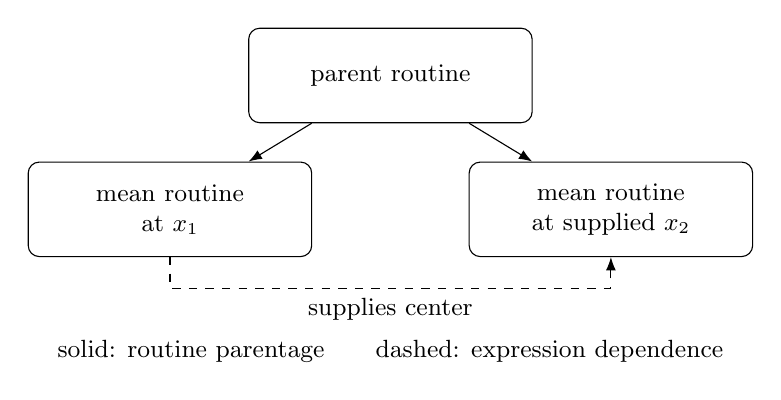
\begin{tikzpicture}[>=Latex,font=\small,
 box/.style={draw,rounded corners,align=center,minimum width=36mm,minimum height=12mm}]
 \node[box] (p) at (0,1.7) {parent routine};
 \node[box] (a) at (-2.8,0) {mean routine\\at $x_1$};
 \node[box] (b) at (2.8,0) {mean routine\\at supplied $x_2$};
 \draw[->] (p)--(a);\draw[->] (p)--(b);
 \draw[->,dashed] (a.south) -- (-2.8,-1) --
 node[below] {supplies center} (2.8,-1) -- (b.south);
 \node[align=center] at (0,-1.8) {solid: routine parentage\qquad dashed: expression dependence};
\end{tikzpicture}
\caption{The two calls have the same routine parent even though
one helps form the other's center.  When a mean occurs twice, each
occurrence uses a separate copy of its entire center-supplying subtree.}
\label{fig:two-depths}
\end{figure}



To evaluate an expression, we expand its mean dependencies as an
uncached tree, duplicating every mean occurrence together with its
entire center-supplying subtree.  All mean calls at any expression tier
are direct children of the routine whose circuit is being evaluated.

The children of a parent labeled $(b,p)$ receive labels as follows:
\begin{equation}
 \begin{array}{c|c}
 \text{child's role}&\text{child labels}\\ \hline
 \text{term of }E_f\text{ in an }\mathsf M\text{ parent}&(b+t,p)\\
 \text{term of }E_f\text{ in an }\mathsf S\text{ parent}&(b,p)\\
 \text{any other term, or the }\mathsf M\text{ position anchor}
       &(b-10t,p-1/4).
 \end{array}
 \label{eq:compiler-labels}
\end{equation}
In the last row the labels are always those of the parent routine,
not successively decreased while descending its expression tree.

\begin{lemma}[Bounded routine height]
\label{lem:compiler-height}
Starting at $(b,p)=(1,K_0)$, the rules
\eqref{eq:compiler-labels} give a finite routine tree of height at most
a constant $H=H(K_0,t)$.  Every reachable label satisfies $b>1/2$.
\end{lemma}
\begin{proof}
Before $4K_0+1$ decreasing transitions, the total loss in $b$ is less
than $10t(4K_0+1)<1/4$, so $b>3/4$.  At that many transitions,
$p\le K_0-(4K_0+1)/4<0$, forcing termination.  Therefore no branch
can have more such transitions.  Positive transitions increase $b$
by $t$, while a nonterminal satisfies $b<p\le K_0$; their total
number is consequently bounded in terms of $K_0,t$ and the already
bounded total decrease in $b$.  A neutral transition is an
$\mathsf S$-to-$\mathsf M$ transition.  Another neutral transition
requires first reaching another $\mathsf S$, which can occur only
through a decreasing transition.  This bounds the neutral transitions
as well and proves both claims.
\end{proof}

A routine is a deterministic function of its center, scalar
parameters, oracle, and a finite ordered list of $d$-dimensional seed
slots.  Standalone use fills these slots by independent standard
Gaussians.  In addition, each routine will have a deterministic vector
$v$ of scalar coefficients, one per slot, with
\begin{equation}
 \|v\|_2\le D_s,\qquad D_s:=\delta^{-t}.
 \label{eq:shift-budget}
\end{equation}
For \emph{every} fixed seed list, changing $x$ to $x+\Delta$ and
adding $v\otimes\Delta/r$ to the seeds will preserve every physical
query point.  The output of $\mathsf M$ will be unchanged; the
normalized output of $\mathsf S$ will decrease by $\Delta/r$.
These are pathwise properties, not statements restricted to Gaussian
seeds.

Within each call write $u=u_{x,r}$ and $\nu=\nu_{x,r}$.
At a terminal call define
\begin{align*}
 \mathsf M&=g(x+rZ)+\sigma G,\\
 \mathsf S&=Z-rg(x+rZ)+(\sqrt3\eta/2)G_1+(\eta/2)G_2,
\end{align*}
with separate seed slots.  The last term in $\mathsf S$ is its
reserved noise.  Taking $v=-1$ on the $Z$ slot and zero elsewhere
proves the shift property and $\|v\|_2=1$.



\subsection{Evaluating an expression at a noisy center}

Fix a parent circuit and its anchors, and write $M_i=u_{x_i,r_i}$
for its exact mean nodes.  For each expression
$E=b_0+\sum_i a_iM_i$, the operation $\operatorname{Eval}(E,n)$
will approximate its exact value plus an independent
$N(0,n^2I_d)$ noise.  Assign disjoint seed blocks to every term
occurrence, its center-supplying computation, and each residual noise;
keep all these blocks separate from the anchors.  Thus the term
blocks are independent conditional on the anchors in a standalone
call.

Here is the recursive evaluation rule, assuming the child routines
and their shift vectors have already been constructed.  Take $A'=A$
for a center expression and $A'=A_f$ at the output, and put
$\sigma_i=n/(2A')$.  For the term of scale $r_i=r\tau_i$, first
evaluate its center expression with noise
\begin{equation}
 n_i=\frac{r_i}{2D_s}.
 \label{eq:compiler-center-noise}
\end{equation}
At this supplied center run the child $\mathsf M$ with scale $r_i$,
noise $\sigma_i$, and labels from \eqref{eq:compiler-labels}.
If its shift vector is $v_i$, apply to its fresh seed block $G_i$
the deterministic slot-space transformation
\begin{equation}
 P_i=\left(I-\frac{v_iv_i^T}{4D_s^2}\right)^{1/2},
 \qquad\text{and use seeds }(P_i\otimes I_d)G_i.
 \label{eq:compiler-seed-transform}
\end{equation}
Denote its output by $Q_i$.  Return
\begin{equation}
 b_0+\sum_i a_iQ_i+
 \left(n^2-\sum_i a_i^2\sigma_i^2\right)^{1/2}G_E,
 \label{eq:compiler-eval}
\end{equation}
where $G_E$ is a separate slot.  The square root is defined, since
\[
 \sum_i a_i^2\sigma_i^2
 \le\left(\sum_i|a_i|\right)^2\frac{n^2}{4(A')^2}
 \le n^2/4.
\]
If there are no terms, return $b_0+nG_E$.  The mean-node ordering
makes the expression recursion finite.  At the parent's output use
the value of $n$ specified above; add the reserved noise for
$\mathsf S$.  A routine supplied with correlated seeds performs
these same deterministic operations, without any change of rule.

At an ideal supplied center $x_i+n_iZ$, Lemma~\ref{lem:compiler-absorption}
now identifies this child with its standalone law at $x_i$.  We still
owe the construction of the shift vectors and a proof that the noisy
supplied centers are accurate.  We prove these in that order.

\subsection{Query-preserving shifts and the deterministic cap}

We next show that the shift vectors required in
Lemma~\ref{lem:compiler-absorption} exist with the universal bound
\eqref{eq:shift-budget}.  This also verifies that the definition is
noncircular and has a deterministic query cap.

For a nonterminal $\mathsf S$, shift its Gaussian position anchor by
$-\rho_e\Delta/r$.  For a nonterminal $\mathsf M$, we require its
position anchor $y_*$ to shift by $-\Delta/(b_*r)$ and leave its
momentum anchor unchanged.  To obtain this, apply the shift of its anchor
$\mathsf S$ call and additionally shift that call's reserved seed
by the coefficient $-2R/b_*$ times $\Delta/r$.  The ordinary shift
changes its output by $-\Delta/r$.  Since the reserved standard
deviation is $R/(2b_*)$, the additional change is
$-R^2\Delta/(b_*^2r)$.  Multiplication by $b_*$ makes the total
change
\[
 -\left(b_*+\frac{R^2}{b_*}\right)\frac{\Delta}{r}
 =-\frac{\Delta}{b_*r}.
\]
The extra slot is used in no query, so query invariance is preserved.

For a term of scale $r\tau_i$, the direct part of its supplied
center then changes by $k_i\Delta$, where
\[
 k_i=1-\ell_i\rho_e\quad(\mathsf S),
 \qquad
 k_i=1-\ell_i/b_*\quad(\mathsf M).
\]
These coefficients satisfy $|k_i|/\tau_i\le C$.  For $\mathsf S$,
$\rho_i\le\rho_e$ gives
$1-\rho_i\rho_e\le2(1-\rho_i)\le2\tau_i$.
For $\mathsf M$, its two possible coefficients obey
\[
 0\le1-\rho_i\cos z/b_*
 \le C(1-\rho_i)+Cz^2,
\]
with $z=0$ when there is no cosine.  Use
$1-\rho_i\le\tau_i$, $\tau_i\ge cR$, and
$z^2/R\le C\delta^{7t}\to0$.

Shift that child's untransformed seed block by
\begin{equation}
 \frac{k_i}{\tau_i}P_i^{-1}v_i\otimes\frac{\Delta}{r}.
 \label{eq:compiler-child-shift}
\end{equation}
If \eqref{eq:shift-budget} holds for the child, the smallest
eigenvalue of $P_i$ is at least $\sqrt3/2$, so
$\|P_i^{-1}\|_{\op}\le2$.  Formula
\eqref{eq:compiler-child-shift} induces exactly the child's shift
for center displacement $k_i\Delta$.  Leave all residual noise
slots fixed.  Induction from leaf expressions upward shows that
every mean output is unchanged, and therefore that the actual
supplied-center change is precisely its direct-term change.
All queries are preserved.  The parent's final direct term is
unchanged for $\mathsf M$ and changes by $-\Delta/r$ for
$\mathsf S$, giving the required output behavior.

The center-supplying subtree and the invoked child have disjoint
slots.  In particular, the factor $k_i/\tau_i$ in
\eqref{eq:compiler-child-shift} multiplies only the shift of that
child, not the shifts of routines used to supply its center.  Those
are other direct children of the same parent and are charged once
in its total shift vector.

\begin{lemma}[Well-defined construction and query cap]
\label{lem:compiler-count}
One can choose $w>0$, depending only on $K_0,t$ and the fixed Picard
counts, and then choose the interpolation orders, so that the entire
construction is well defined for all sufficiently large $d$.
Every routine reached from a top call satisfies
\eqref{eq:shift-budget}.  Its total number of seed slots and oracle
queries is at most $\polylog(d)\delta^{-t}$ on every execution.
\end{lemma}
\begin{proof}
Let $D_0$ be the dependency-depth bound in
Theorem~\ref{thm:numerical-interface}, and let $F_0$ be its direct
fan-out bound.  Expanding a circuit into an expression tree costs
at most $(D_0+1)(1+F_0)^{D_0}$ nodes.  Its size is thus
$\polylog(d)\delta^{-C_2w}$, where $C_2$ depends on the Picard
counts but not on $w$ or the interpolation orders.  This bounds its
direct child invocations and its own anchor and residual slots.
Expanding through the height $H$ from
Lemma~\ref{lem:compiler-height} gives
$\polylog(d)\delta^{-C_3w}$ slots and terminal queries.
Interpolation orders change only fixed multiplicative constants in
these bounds, not $C_2$ or $C_3$.

The terminal shift has norm $1$.  Assuming the shift bound for the
children, the bounded ratios and inverse norms above show that a
parent's shift norm is at most a fixed constant times one plus the
sum of its direct children's shift norms, including the anchor
call.  The extra reserved-slot shift has bounded coefficient.
The triangle inequality is sufficient even if ordinary and extra
anchor shifts affect the same slot.  Iterating through the fixed
routine height gives the same bound
$\polylog(d)\delta^{-C_3w}$, after increasing $C_3$ if necessary.

Choose $w>0$ with
\[
 C_3w<t/2,\qquad w<t,\qquad c_1w<t,
\]
and only then choose the fixed interpolation orders needed in
Theorem~\ref{thm:numerical-interface}.  For sufficiently large $d$, the last
shift bound is smaller than $D_s=\delta^{-t}$.  This is a valid
bottom-up induction: it proves each child's bound before using its
inverse transformation in the parent.  The count bound is also at
most $\polylog(d)\delta^{-t}$.

To make the parameter order explicit, first fix the Picard counts,
hence $D_0,H,C_3$, then $w$, then the interpolation orders.  The
universal scalar $D_s$ fixes every center-noise budget.  The circuit
shapes, labels, requested noises, and slot counts are determined by
these scalar parameters before any shifts are computed.  Compute
child shifts before their matrices and the parent shift.  No center
value, oracle response, numerical-error estimate, or assumption
\eqref{eq:routine-sizes} enters this finite construction or the
count.  Only terminal routines query $g$, once each; hence the bound
is a cap on every execution, not an expected query count.
\end{proof}

\subsection{Terminal errors and propagation of scales}

The finite construction and its cap are now established independently
of accuracy.  We next verify its terminal errors and the size conditions
needed by the numerical estimates.

\begin{lemma}[Terminal accuracy]
\label{lem:compiler-terminal}
In standalone use, a terminal call satisfying \eqref{eq:routine-sizes}
obeys
\begin{align*}
 W_2\bigl(\mathcal L(\mathsf M),N(u,\sigma^2I_d)\bigr)
 &\le\polylog(d)\sigma\delta^pD(x),\\
 W_2\bigl(\mathcal L(\mathsf S_{\rm pre}),
          \nu_{x,r}*N(0,3\eta^2I_d/4)\bigr)
 &\le\polylog(d)\delta^pD(x),
\end{align*}
where $\mathsf S_{\rm pre}$ is the output before adding its reserved
noise $\eta G_2/2$.  The sampling bound also holds after adding that
same independent reserve to both laws.  The fixed-seed center
Lipschitz constant is at most $\lambda$ for $\mathsf M$ and
$r\lambda$ for $\mathsf S$.
\end{lemma}
\begin{proof}
For the standard Gaussian seed $Z$, the primitive moment bounds give
\[
 \|g(x+rZ)-u\|_{L^2}
 \le CL\bigl(\sqrt d+r|g(x)|\bigr)\le CLD(x).
\]
Since $L/\sigma\le\polylog(d)\delta^b$ and $p\le b$, this is
within the mean error budget; couple the added Gaussian identically.

Let $z_0$ be the mode of $\nu_{x,r}$, so
$z_0=-rg(x+rz_0)$.  Then
\[
 \|Z-rg(x+rZ)-(Z+z_0)\|_{L^2}
 \le l\|Z-z_0\|_{L^2}\le ClD(x).
\]
Also $W_2(N(z_0,I_d),\nu_{x,r})\le Cl\sqrt d$.
Apply the synchronous comparison in
Lemma~\ref{lem:convex-preliminaries} with Gaussian potential
$H_0(z)=|z-z_0|^2/2$ (contraction constant $1$) and tilted potential
$H(z)=|z|^2/2+F(x+rz)$.  Their gradient difference is
$r[g(x+rz)-g(x+rz_0)]$, whose $L^2(\nu_{x,r})$ norm is at most
$l\|Z-z_0\|_{L^2(\nu_{x,r})}\le Cl\sqrt d$.
This proves the displayed Wasserstein bound under exactly the
$C^2$ and bounded-Hessian hypotheses of that lemma.
Adding the same independent comparison noises proves the sampling
error $ClD(x)\le\polylog(d)\eta\delta^bD(x)$, which is at most
the requested bound because $\eta\le1$ and $p\le b$.  Omitting
$G_2$ proves the pre-reserved assertion.  The Lipschitz bounds follow
directly from the two displayed terminal formulas.
\end{proof}

\begin{lemma}[Size conditions descend through the routine tree]
\label{lem:compiler-sizes}
Starting with a top call satisfying
\eqref{eq:routine-sizes}, every descendant satisfies that condition
with its assigned labels, up to a uniform polylogarithmic factor.
At each nonterminal circuit,
\begin{equation}
 \lambda A\le\polylog(d)\delta^{1/3}.
 \label{eq:small-coefficients}
\end{equation}
For nonfinal expression terms within an $\mathsf M$ parent,
$\sigma_i\le C\sigma$; within an $\mathsf S$ parent,
$r\sigma_i\le C$.
\end{lemma}
\begin{proof}
For a final term of an $\mathsf M$ parent, the output uses only means of scale $rR$, so $r_i=rR$, while $\sigma_i$ is a fixed positive multiple
of $\sigma$.  Thus $L_i/\sigma_i$ gains a factor $R$ and $l_i$
gains $R^2$, allowing labels $(b+t,p)$.
For a final term of an $\mathsf S$ parent,
$\sigma_i$ is a fixed positive multiple of $\eta/r$.
Therefore $L_i/\sigma_i\le Cl/\eta$ and $l_i\le l$, allowing
the unchanged labels.

For a nonfinal term, let $r\tau_{\rm prev}$ be the scale of the
node whose center is currently being supplied.  Its expression is
evaluated with budget $r\tau_{\rm prev}/(2D_s)$, irrespective of
the tier at which it occurs.  Consequently
\[
 \sigma_i=\frac{r\tau_{\rm prev}}{4D_sA},
 \qquad
 \frac{L_i}{\sigma_i}
 \le \frac{CD_s\lambda A}{R}.
\]
The coefficient estimates give
$\lambda A\le\polylog(d)\delta^{b-4t-c_1w}$ for an
$\mathsf M$ parent.  For an $\mathsf S$ parent,
$\lambda A=C_1l\le\polylog(d)\delta^b$, since $\eta\le1$.
Using $D_s/R=\delta^{-2t}$ and $c_1w<t$ costs less than the
allowed $10t$ decrease in $b$.  Also $l_i\le l$.
For the position-anchor $\mathsf S$ call of $\mathsf M$,
$l/\eta\le l/R$, which has the same allowance.
This proves the size conditions by the bounded routine height.
All accumulated fixed and polylogarithmic factors are still one
polylogarithmic factor.

As $b>1/2$ and $4t+c_1w<5t<1/6$, the coefficient bounds imply
\eqref{eq:small-coefficients}.  Finally, the positive declared bound
for $A$ includes a fixed multiple of $r/\sigma$ in an
$\mathsf M$ parent, so
$\sigma_i\le r/(4D_sA)\le C\sigma$.
For $\mathsf S$, $A=C_1r^2$ gives
$r\sigma_i\le1/(4C_1D_s)\le C$.
\end{proof}

\subsection{Stability for arbitrary fixed seeds}

\begin{lemma}[Fixed-seed stability]
\label{lem:compiler-lipschitz}
For every seed array, including correlated or transformed arrays,
the compiled $\mathsf M$ output is a function of $x$ with Lipschitz
constant at most $\polylog(d)\lambda$; the normalized
$\mathsf S$ output has constant at most
$\polylog(d)r\lambda$.  If the anchors of a nonterminal
$\mathsf M$ are treated as separate inputs, its Lipschitz constant
in the position anchor is at most $\polylog(d)L$.
\end{lemma}
\begin{proof}
Induct on routine height, with the terminal case supplied by
Lemma~\ref{lem:compiler-terminal}.  First hold the anchors fixed.
A direct center term has Lipschitz constant $1$ in $x$ and at most
$Cr$ in a position anchor.  The center-supplying expression combines
child outputs with total absolute coefficient at most $A$.
Using the child $\mathsf M$ bound, the contribution of earlier
supplied-center sensitivities is at most
$\polylog(d)\lambda A$ times their maximum.  By
\eqref{eq:small-coefficients}, this is small.  Induction through
the bounded expression depth therefore bounds center sensitivities
by a constant times their direct sensitivities, with an allowed
polylogarithmic factor.

At the final expression the coefficient sum is $A_f$.  Its direct
term has no center dependence when anchors are held fixed; for
$\mathsf M$ it also has no position-anchor dependence.  Hence its
center sensitivity is at most
$\polylog(d)A_f\lambda$, and its $\mathsf M$ position-anchor
sensitivity at most $\polylog(d)A_f\lambda r$.
These are the asserted bounds with anchors treated as separate inputs.
The $\mathsf S$ Gaussian anchor is indeed center independent.
The $\mathsf M$ position anchor is supplied by $\mathsf S$ at
the same center, whose center Lipschitz constant by induction is
$\polylog(d)r\lambda$.  Its additional contribution is at most
$\polylog(d)Lr\lambda=\polylog(d)L^2$, and
$L^2\le\lambda$ for $r\le1$ and $\lambda\le1$.
All seed transformations depend only on scalar parameters, not on
$x$.  The proof uses only fixed-seed identities and Lipschitz
bounds, and therefore requires no seed independence.
\end{proof}

\subsection{Standalone accuracy and the primitive theorem}

We prove the law guarantees by induction on routine height.  This is
the only stage at which a routine's seeds are assumed independent
standard Gaussians.  Such an assumption will be used for a child only
after the absorption identity has restored its full standalone seed
law.

\begin{proposition}[Accuracy of the compiled routines]
\label{prop:compiler-accuracy}
For every call reached from the top labels, the standalone routines
satisfy
\begin{align*}
 W_2(\mathcal L(\mathsf M),N(u,\sigma^2I_d))
 &\le\polylog(d)\sigma\delta^pD(x),\\
 W_2\bigl(\mathcal L(\mathsf S_{\rm pre}),
       \nu_{x,r}*N(0,3\eta^2I_d/4)\bigr)
 &\le\polylog(d)\delta^pD(x),
\end{align*}
where $\mathsf S_{\rm pre}$ denotes the output before its reserved
noise.  The latter bound also holds after adding the reserved noise
to both laws, and
\[
 \|\mathcal L(\mathsf S)-\nu_{x,r}*N(0,\eta^2I_d)\|_{\TV}
 \le\polylog(d)\frac{\delta^pD(x)}{\eta}.
\]
\end{proposition}

\begin{proof}
The terminal assertion is Lemma~\ref{lem:compiler-terminal}.
All random variables below have finite second moments: the actual
algorithms are finite compositions of affine maps and globally
Lipschitz oracle evaluations, while ideal tilted variables have the
primitive moment bounds.  Thus all $W_2$ comparisons are defined.

For a nonterminal $\mathsf M$, first couple its approximate
$\mathsf S$ position anchor to an ideal anchor, independently of
all remaining seed blocks.  The child labels are
$(b-10t,p-1/4)$.  By induction and
Lemma~\ref{lem:compiler-lipschitz}, replacing this anchor costs at
most
\[
 \polylog(d)L\delta^{p-1/4}D(x).
\]
After division by the mean error unit $\sigma\delta^pD(x)$,
the cost is at most
$\polylog(d)\delta^{b-1/4}$, hence is bounded for large $d$.
We may now assume that the position anchor has law $b_*Z+RN$,
where $Z\sim\nu_{x,r}$ and $N$ is standard Gaussian, and that the
momentum anchor is an independent standard Gaussian.  These are exactly
the input laws in Theorem~\ref{thm:numerical-interface}.

Let $x_i$ be the centers of the deterministic exact-mean circuit
under these anchors, and put $D_i=\sqrt d+|g(x_i)|$.
Their RMS values over anchors obey
\begin{equation}
 \max_i\|D_i\|_{L^2}\le\polylog(d)D(x).
 \label{eq:compiler-center-moments}
\end{equation}
Indeed, both position and momentum anchors have RMS at most $CD(x)$.
Use $|g(x_i)|\le|g(x)|+\lambda|x_i-x|$ and the circuit's
direct terms.  An exact primitive mean at a preceding center has
magnitude at most $CD_j$.  Their contribution to this maximum-of-RMS
recurrence is at most $C\lambda A$ times its previous maximum.
This is small by \eqref{eq:small-coefficients}; the direct terms cost
at most $CD(x)$.  Induction through the node ordering proves
\eqref{eq:compiler-center-moments} without a maximum inside the
expectation.

Condition on the anchors.  For an expression $E$, write
$\epsilon_E$ for the $W_2$ error of
$\operatorname{Eval}(E,n)$ relative to its deterministic exact
value plus $N(0,n^2I_d)$.  Couple the supplied center of its $i$th
term to $x_i+n_iZ$ with its conditional $W_2$ error
$\epsilon_{E_i}$.  Use the same transformed child seeds on these
two centers, drawn independently of this coupling.  The fixed-seed
Lipschitz bound costs at most
$\polylog(d)\lambda\epsilon_{E_i}$.
At the ideal noisy center, Lemma~\ref{lem:compiler-absorption}
identifies the child's law with its standalone law at $x_i$.
The induction hypothesis therefore supplies the additional error
$\polylog(d)\sigma_i\delta^{p_i}D_i$.

Different term occurrences have disjoint blocks, so their outputs
are independent conditional on the anchors.  Product couplings
compare them to independent noised exact means.  Together with the
independent residual in \eqref{eq:compiler-eval}, the ideal sum
has exactly covariance $n^2I_d$.  We conclude that
\begin{equation}
 \epsilon_E\le\sum_i|a_i|
 \left[\polylog(d)\lambda\epsilon_{E_i}
       +\polylog(d)\sigma_i\delta^{p_i}D_i\right].
 \label{eq:compiler-error-recursion}
\end{equation}
Notice the order of this argument: inaccurate supplied centers use
only pathwise stability, and standalone accuracy is invoked only
after Gaussian absorption.  No assertion is made that the actual
algorithm's intermediate states have the ideal input laws.

Take RMS in the anchors and expand
\eqref{eq:compiler-error-recursion} through the finite expression
tree.  At its root, direct-child labels have $p_i=p$ and
\[
 \sum_i|a_i|\sigma_i
 \le A_f\frac{n}{2A_f}=n/2.
\]
Thus their intrinsic errors fit the requested budget.  At tier
$j\ge2$, absolute coefficient sums and Lipschitz factors contribute
at most
\[
 A_f\bigl(\polylog(d)\lambda A\bigr)^{j-1}.
\]
All such children have the single accuracy-label loss $p_i=p-1/4$,
not one loss per expression tier.  Their noise units are at most
$C\sigma$ in an $\mathsf M$ parent and $C/r$ in an
$\mathsf S$ parent by Lemma~\ref{lem:compiler-sizes}; these units
combine with $A_f=C_1$ or $C_1r$, respectively.
Already the first factor
$\polylog(d)\lambda A\le\polylog(d)\delta^{1/3}$
pays for the loss $\delta^{-1/4}$, leaving a positive power
$\delta^{1/12}$.  The bounded expression depth allows all further
tiers and polylogarithmic factors to be summed.  Leaf affine
expressions have zero error.  This proves the required final
evaluation error.

Conditionally on the anchors, the ideal final evaluation is its
deterministic exact-mean circuit value plus a Gaussian of the
specified fixed covariance.  Its noise may therefore be taken
independent of the anchors.  By Lemma~\ref{lem:compiler-sizes},
Theorem~\ref{thm:numerical-interface} applies.  It compares the ideal mean
circuit to $N(u,\sigma^2I_d/4)$ and the ideal sampling circuit to
$\nu_{x,r}*N(0,\eta^2I_d/4)$, with the respective errors
$\polylog(d)\sigma\delta^JD(x)$ and
$\polylog(d)\delta^JD(x)$.  Since $J=K_0+2$ and $p\le K_0$,
both errors fit the requested bounds.
Couple the independent evaluation noise identically in each comparison.
For $\mathsf M$, its variance $3\sigma^2/4$ raises the Gaussian
target variance from $\sigma^2/4$ to $\sigma^2$.
For $\mathsf S$, its variance $\eta^2/2$ raises the Gaussian
convolution variance from $\eta^2/4$ to $3\eta^2/4$.
This closes the standalone induction.  Adding the common reserved
noise preserves the $W_2$ bound; Gaussian smoothing by its standard
deviation $\eta/2$ gives the stated total variation bound by
\eqref{eq:gaussian-smoothing}.
\end{proof}

\begin{proof}[Proof of Theorem~\ref{thm:primitive}]
Use the top $\mathsf S$ call with $(b,p,\eta)=(1,K_0,1)$.
Because $l=\delta r^2\le\delta$, its size condition holds with
constant $1$.  Proposition~\ref{prop:compiler-accuracy} gives both
$W_2$ and total variation error at most
$\polylog(d)\delta^{K_0}D(x)$ from
$\nu_{x,r}*N(0,I_d)$, uniformly in $x$ and $0<r\le1$.
Lemma~\ref{lem:compiler-count} gives at most
$\polylog(d)\delta^{-t}$ evaluations of $g$ on every execution.
The output has the form $X_{\rm pre}+G/2$, where the reserved standard
Gaussian $G$ is independent of $X_{\rm pre}$ and all queries, and the
pre-reserved conclusion of Proposition~\ref{prop:compiler-accuracy}
gives $W_2(\mathcal L(X_{\rm pre}),\nu_{x,r}*N(0,3I_d/4))
\le\polylog(d)\delta^{K_0}D(x)$.
The exact means and numerical comparison laws serve only to analyze this finite
algorithm; its only oracle operations are the terminal evaluations.
\end{proof}

\section{From noisy conditional samples to the target law}
\label{sec:sampling}

The auxiliary algorithm returns a conditional sample with an added
Gaussian. We now use it to sample the original, unnoised law
$\pi_V$. The construction has two stages. A contracting proximal chain
first approaches $\widetilde\pi=\pi_V*N(0,hI_d)$. Conditional on its
output, a sequence of variance-halving steps reduces the remaining
sampling problem to a law close to a mode-centered Gaussian. The
numbers of calls in both stages are prescribed in advance.

Throughout this section, $V\in C^2(\R^d)$ satisfies
$V(0)=0$, $\nabla V(0)=0$, and
$I_d\preceq\nabla^2V\preceq2I_d$ everywhere. The origin is therefore
the supplied minimizer. Each original query returns both $V$ and
$\nabla V$ at the queried point. The main construction uses only the
gradient; the bounded-dimensional fallback also uses the value.
We fix $0<e<1$, put $\delta=d^{-e}$ and $h=\delta/2$, and take an
integer $K_0>2+1/e$. Choose $t>0$ as in \eqref{eq:t-choice}, and
fix the approximation orders required by Theorem~\ref{thm:primitive}.
All sufficiently-large-dimension thresholds below are uniform in $V$.

\subsection{A contracting noised chain}

The Gaussian proximal sampler alternates a Gaussian step with a
restricted Gaussian conditional draw
\citep[Definition~1 and Lemmas~2 and~4]{lee2021proximal}; see also
\citet[Section~3 and Theorem~1]{chen2022proximal}. We use the chain
on the noised variable and prove its contraction directly.

For $y\in\R^d$, denote by $\kappa_y$ the probability law with density
proportional to
\begin{equation}\label{eq:proximal-conditional}
              \exp\!\left(-V(x')-\frac{|x'-y|^2}{2h}\right).
\end{equation}
The ideal transition $P_h$ draws $x'\sim\kappa_y$ and returns
$x'+\sqrt h\,N$, where $N$ is an independent standard Gaussian.
Thus $P_h(y,\cdot)=\kappa_y*N(0,hI_d)$.

\begin{lemma}[Proximal contraction]\label{lem:proximal-contraction}
The law $\widetilde\pi$ is invariant for $P_h$, and
\[
 \Wtwo(\kappa_{y_1},\kappa_{y_2})
       \le\frac{|y_1-y_2|}{1+h}.
\]
Consequently, for input laws $\mu,\eta$ of finite second moment,
\[
 \Wtwo(\mu P_h,\eta P_h)
       \le\frac{\Wtwo(\mu,\eta)}{1+h}.
\]
\end{lemma}
\begin{proof}
Under the joint law $\pi_V(dx)N(x,hI_d)(dy)$, the conditional law
of $x$ given $y$ is $\kappa_y$. Drawing this conditional and then
redrawing $y$ given $x$ preserves the joint law, whose $y$-marginal
is $\widetilde\pi$.

The potential in \eqref{eq:proximal-conditional} has curvature at
least $1+1/h$. Replacing $y_1$ by $y_2$ changes its gradient by the
constant vector $(y_1-y_2)/h$. The synchronous comparison
\eqref{eq:synchronous-comparison} therefore bounds the conditional
$\Wtwo$ distance by $|y_1-y_2|/(1+h)$. Couple the subsequent Gaussian
increments identically. Integrating these conditional couplings
against an input coupling, as in Lemma~\ref{lem:coupling-smoothing},
proves the kernel contraction.
\end{proof}

To implement this transition, substitute $x'=y+\sqrt h\,z$ in
\eqref{eq:proximal-conditional}. The normalized conditional potential
becomes $|z|^2/2+F_y(z)$, where
\begin{equation}\label{eq:proximal-primitive}
 F_y(z)=V(y+\sqrt h\,z),\qquad
 g_y(z)=\nabla F_y(z)=\sqrt h\,\nabla V(y+\sqrt h\,z).
\end{equation}
The Hessian bound and $\nabla V(0)=0$ give
\[
 \Lip(g_y)\le2h=\delta,\qquad |g_y(0)|\le2\sqrt h\,|y|.
\]
An evaluation of $g_y$ is one original first-order query. Apply
Theorem~\ref{thm:primitive} to $F_y$ at center zero and scale one,
with fresh standalone seeds, and map its output $S$ to
$y+\sqrt h\,S$. This defines the actual transition $\widehat P_h$.
The primitive already approximates $Z+N$, so the ideal comparison
law of this affine image is exactly $P_h(y,\cdot)$.
In particular, the primitive's independent final reserve $G/2$
is retained. Its pre-reserve $\Wtwo$ guarantee and Gaussian smoothing
are what supply the following TV guarantee:
\begin{equation}\label{eq:proximal-local-errors}
 \begin{aligned}
 \Wtwo(\widehat P_h(y,\cdot),P_h(y,\cdot))
   &\le\sqrt h\,B_d\delta^{K_0}
                    (\sqrt d+2\sqrt h\,|y|),\\
 \norm{\widehat P_h(y,\cdot)-P_h(y,\cdot)}_{\TV}
   &\le B_d\delta^{K_0}(\sqrt d+2\sqrt h\,|y|).
 \end{aligned}
\end{equation}
Here and below $B_d=C(1+\log d)^C$ may be increased by a fixed
factor or power. Its constants depend only on the fixed parameters,
not on the center, oracle, or random history.

\begin{proposition}[Mixing of the approximate noised chain]
\label{prop:noised-mixing}
With $K_0>2+1/e$ and $t$ chosen above, start the
$\widehat P_h$-chain at zero and run
$\lceil Ch^{-1}\log d\rceil+1$ steps. For a sufficiently large
fixed $C$, its output has total-variation distance $o(1)$ from
$\widetilde\pi$, uniformly over all admissible $V$.
\end{proposition}
\begin{proof}
Lemma~\ref{lem:convex-preliminaries}, applied at the mode zero,
gives $\E_{\pi_V}|X|^2\le d$. Hence the root mean square under
$\widetilde\pi$ is at most $C\sqrt d$.
Let $\mu_k$ be the actual law after $k$ steps, and set
$a_k=\Wtwo(\mu_k,\widetilde\pi)$. Then
\[
 \left(\int |y|^2\,\mu_k(dy)\right)^{1/2}
       \le a_k+C\sqrt d.
\]
All these moments are finite. Indeed they are finite at $k=0$, and
the local $\Wtwo$ bound in \eqref{eq:proximal-local-errors}, together
with the conditional moment bounds for $P_h$, propagates finite
second moments to the next step.

Take the root mean square of the first local error in
\eqref{eq:proximal-local-errors}. Conditional coupling and
Lemma~\ref{lem:proximal-contraction} give
\[
 a_{k+1}\le
 \left(\frac1{1+h}+2hB_d\delta^{K_0}\right)a_k
       +C\sqrt h\,B_d\delta^{K_0}\sqrt d.
\]
For all large $d$, the coefficient of $a_k$ is at most $1-ch$
for an absolute $c>0$. Since $a_0\le C\sqrt d$, summing this
geometric recurrence yields
\begin{equation}\label{eq:proximal-global-error}
 a_k\le C\sqrt d\,e^{-chk}
       +Ch^{-1/2}B_d\delta^{K_0}\sqrt d.
\end{equation}
The second term is $o(\sqrt h)$: after division by $\sqrt h$,
it is bounded by a constant times
$B_d\delta^{K_0-1}\sqrt d$, which tends to zero because
$e(K_0-1)>1/2$. At $k=\lceil Ch^{-1}\log d\rceil$, a sufficiently
large fixed $C$ makes the first term $o(\sqrt h)$ as well.

Use one more transition to obtain TV control. The mixture bound
in Lemma~\ref{lem:coupling-smoothing} gives
\[
 \norm{\mu_k\widehat P_h-\mu_kP_h}_{\TV}
 \le B_d\delta^{K_0}
       \bigl[\sqrt d+2\sqrt h\,(a_k+C\sqrt d)\bigr]=o(1).
\]
For the remaining comparison, the conditional $x'$-laws from
$\mu_k$ and $\widetilde\pi$ can be coupled with root mean square
at most $a_k/(1+h)$. Their common independent $\sqrt h$-Gaussian
then gives, by \eqref{eq:gaussian-smoothing},
\[
 \norm{\mu_kP_h-\widetilde\pi P_h}_{\TV}
       \le\frac{a_k}{(1+h)\sqrt h}=o(1).
\]
Invariance of $\widetilde\pi$ completes the proof.
\end{proof}

\subsection{Conditional descent and its ideal histories}

An exact draw from $\kappa_y$ with $y\sim\widetilde\pi$ has
marginal $\pi_V$. We next implement this unnoised conditional draw.
For its analysis, first replace the incoming approximate $y$ by
$y\sim\widetilde\pi$. Applying the same conditional algorithm to
both inputs costs at most the TV error of
Proposition~\ref{prop:noised-mixing}, by data processing.

For a related recursive restricted-Gaussian-oracle framework, see
Chen--Chewi--Lu--Zhang \cite[Algorithm~3.3 and Section~6.3]{chen2026picard}.
The construction here uses fixed variance halving, mode-centered Gaussian
termination, and an every-execution query cap.

Fix $y$ temporarily. Keep $F_y$ and its oracle $g_y$ fixed throughout
the conditional algorithm; only the primitive center and scale
change. At center $x$ and scale $r$, the desired normalized law is
\[
 \nu_{x,r}(dz)\propto
             \exp\bigl(-|z|^2/2-F_y(x+rz)\bigr)\,dz.
\]
Suppose first that $Z\sim\nu_{x,r}$ and that $N$ is an independent
standard Gaussian. Given $Y=Z+N$, the conditional density of $Z$
is proportional to
\[
             \exp\bigl(-|z-Y/2|^2-F_y(x+rz)\bigr).
\]
Substitute $z=Y/2+z_{\rm new}/\sqrt2$ to obtain the exact identity
\begin{equation}\label{eq:conditional-descent}
 Z=\frac Y2+\frac{Z_{\rm new}}{\sqrt2},\qquad
 Z_{\rm new}\mid Y\sim\nu_{\,x+rY/2,\;r/\sqrt2}.
\end{equation}

The actual algorithm starts at $x_0=0,r_0=1$ and uses
$J=\lceil C_1\log d\rceil$ levels. At each $0\le j<J$, it calls
Theorem~\ref{thm:primitive} with fresh seeds at $(x_j,r_j)$ to
produce a noised observation $Y_j$, and sets
\[
 x_{j+1}=x_j+r_jY_j/2,\qquad r_{j+1}=r_j/\sqrt2.
\]
At level $J$, it produces a base sample $Z_J$ by the Gaussian
rule given below and returns
\[
                         y+\sqrt h\,(x_J+r_JZ_J).
\]
To identify this output, define the backwards variables
$Z_j=Y_j/2+Z_{j+1}/\sqrt2$ for the analysis. The center update gives
\[
 x_j+r_jZ_j
 =x_j+r_jY_j/2+(r_j/\sqrt2)Z_{j+1}
 =x_{j+1}+r_{j+1}Z_{j+1}.
\]
Since $x_0=0$ and $r_0=1$, the returned point is therefore
$y+\sqrt h\,Z_0$. By \eqref{eq:conditional-descent}, ideal
observations and an exact base conditional sample would make this
an exact draw from $\kappa_y$.

We must control the errors at random centers. The useful moment
bound concerns the history in which all preceding observations
have their ideal laws.

\begin{lemma}[Moments along the ideal descent]
\label{lem:descent-moments}
If $y\sim\widetilde\pi$ and every conditioning observation preceding
level $j$ is ideal, then
\[
 b_j:=\left(\E|g_y(x_j)|^2\right)^{1/2}\le C\sqrt d
             \qquad(0\le j\le J),
\]
with an absolute $C$ for all sufficiently large $d$.
\end{lemma}
\begin{proof}
The initial estimate follows from
$|g_y(0)|\le2\sqrt h\,|y|$ and the moment bound for
$\widetilde\pi$. Conditional on an ideal history, the next
observation has the law of $Z+N$ at center $x_j$ and scale
$r_j=2^{-j/2}$. Equation~\eqref{eq:primitive-moments} therefore gives
\[
 \left(\E[|Y_j|^2\mid x_j,y]\right)^{1/2}
          \le C(\sqrt d+r_j|g_y(x_j)|).
\]
The center update and $\Lip(g_y)\le\delta$ imply, by the
conditional and then unconditional $L^2$ triangle inequalities,
\[
 b_{j+1}\le(1+C\delta r_j^2)b_j+C\delta r_j\sqrt d.
\]
Both $\sum_{j\ge0}r_j$ and $\sum_{j\ge0}r_j^2$ are bounded
by absolute constants. In particular the products of
$1+C\delta r_j^2$ are bounded by
$\exp(C\delta\sum_jr_j^2)$. Expanding the recurrence proves
the stated uniform bound.
\end{proof}

Here is the precise replacement order used to sum the TV errors.
For $0\le j\le J$, let $H_j$ be the output law when the first
$j$ observations are ideal, all later observations use the actual
primitive, and the base rule is the actual Gaussian rule.
For $0\le j<J$, the laws $H_j$ and $H_{j+1}$ have the same ideal prefix of length
$j$. Conditional on that prefix, only the next observation kernel
changes; all subsequent computation is the same probability kernel.
Data processing and the mixture TV bound therefore give
\[
 \norm{H_j-H_{j+1}}_{\TV}
    \le B_d\delta^{K_0}\E_{\rm ideal}
                        \bigl[\sqrt d+|g_y(x_j)|\bigr].
\]
The expectation includes $y\sim\widetilde\pi$ and the common
ideal prefix. Lemma~\ref{lem:descent-moments} now yields
\begin{equation}\label{eq:descent-tv}
 \norm{H_0-H_J}_{\TV}
       \le CJ B_d\delta^{K_0}\sqrt d=o(1).
\end{equation}
Thus errors are summed using only ideal-history moments. It remains
to compare the actual and exact base laws under that same ideal history.

\subsection{The Gaussian base rule}

At depth $J$, write $l=\delta r_J^2$ and start at $z^{(0)}=0$.
Make exactly $m_0=\lceil C_2\log d\rceil$ gradient iterations
\begin{equation}\label{eq:mode-iteration}
 z^{(k+1)}=-r_Jg_y(x_J+r_Jz^{(k)}),
                         \qquad 0\le k<m_0.
\end{equation}
The base output is $Z_J=z^{(m_0)}+G$, for a fresh standard
Gaussian $G$. The iteration map has Lipschitz constant at most $l$.
Its unique fixed point is the mode $z_0$ of $\nu_{x_J,r_J}$, and
\eqref{eq:primitive-moments} gives
\begin{equation}\label{eq:mode-accuracy}
 |z^{(m_0)}-z_0|
       \le l^{m_0}|z_0|
       \le l^{m_0}\frac{r_J|g_y(x_J)|}{1-l}.
\end{equation}
The following comparison explains why a Gaussian centered there
completes the construction.

\begin{lemma}[Mode-centered Gaussian approximation]
\label{lem:mode-gaussian}
For any $F\in C^2(\R^d)$ with $\Lip(\nabla F)\le\lambda$, center
$x$, and scale $0<r\le1$ such that $l=\lambda r^2\le1/2$, let $z_0$ be
the mode of $\nu_{x,r}$. Then
\[
 \norm{\nu_{x,r}-N(z_0,I_d)}_{\TV}\le Cl\sqrt d.
\]
\end{lemma}
\begin{proof}
Translate by $z_0$. Up to an additive constant, the potential of
$w=z-z_0$ is $|w|^2/2+J(w)$, where
\[
 J(w)=z_0\cdot w+F(x+r(z_0+w))-F(x+rz_0).
\]
The mode equation gives $\nabla J(0)=0$, and
$\Lip(\nabla J)\le l$. In particular $J(0)=0$ and
$|J(w)|\le l|w|^2/2$.
For $0\le s\le1$, the potential $|w|^2/2+sJ(w)$ has mode zero
and Hessian between $(1-l)I_d$ and $(1+l)I_d$.
Its law $\mu_s$ satisfies, by Lemma~\ref{lem:convex-preliminaries},
\[
 \Var_{\mu_s}J
 \le\frac1{1-l}\E_{\mu_s}|\nabla J|^2
 \le\frac{l^2}{1-l}\E_{\mu_s}|w|^2
 \le\frac{l^2d}{(1-l)^2}\le4l^2d.
\]
The same quadratic bounds justify differentiating
\[
 \Phi(s)=\log\int_{\R^d}e^{-|w|^2/2-sJ(w)}\,dw
\]
twice under the integral, and give
$\Phi''(s)=\Var_{\mu_s}J$. Since $\mu_0=N(0,I_d)$,
\[
 \KL(\mu_0\Vert\mu_1)
  =\Phi(1)-\Phi(0)-\Phi'(0)
  =\int_0^1(1-s)\Phi''(s)\,ds\le2l^2d.
\]
Pinsker's inequality, followed by translation back by $z_0$,
proves the assertion.
\end{proof}

Under an ideal history, the Gaussian shift bound and
\eqref{eq:mode-accuracy} bound the expected TV error of the base rule
by
\begin{equation}\label{eq:descent-base-error}
 C\delta 2^{-J}\sqrt d
 +C(\delta2^{-J})^{m_0}
                 \frac{2^{-J/2}\sqrt d}{1-\delta2^{-J}}.
\end{equation}
Here the second term uses Lemma~\ref{lem:descent-moments}.
Choose the fixed $C_1$ large enough that
$\delta2^{-J}\sqrt d\to0$. A sufficiently large fixed $C_2$
makes the second term tend to zero as well. Replacing the base law
under the ideal history therefore changes TV by $o(1)$.
By \eqref{eq:conditional-descent}, the resulting completely ideal
conditional algorithm returns $\kappa_y$. Averaging over
$y\sim\widetilde\pi$ gives $\pi_V$.

Combining this base comparison, \eqref{eq:descent-tv}, and the
initial replacement of the incoming $y$ proves
\begin{equation}\label{eq:unnoised-output-error}
            \norm{\mathcal L(X_{\rm out})-\pi_V}_{\TV}=o(1),
\end{equation}
uniformly over admissible $V$. The final Gaussian is used to
approximate the last conditional law; the law in
\eqref{eq:unnoised-output-error} is the original target without
an additional convolution.

\subsection{Query counts and all dimensions}

\begin{theorem}[Subpolynomial upper bound]\label{thm:upper}
For every fixed $\varepsilon>0$, there is $C_\varepsilon<\infty$
such that, for every integer $d\ge2$, a measurable algorithm using
the exact value-and-gradient oracle makes at most
$C_\varepsilon d^\varepsilon$ queries on every execution and
returns a sample within TV distance $1/10$ of $\pi_V$ for every
$V$ satisfying \eqref{eq:original-class}. Thus
\[
                  Q(d)\le C_\varepsilon d^\varepsilon
                       \qquad(d\ge2).
\]
\end{theorem}
\begin{proof}
Given $\varepsilon>0$, first choose $e\in(0,1)$ with
$2e<\varepsilon$, then an integer $K_0>2+1/e$, and then
$t>0$ satisfying \eqref{eq:t-choice}. Fix the auxiliary construction's
orders in its prescribed order, and finally the constants in the
chain, descent depth, and base iteration count. These choices may
depend on $\varepsilon$, but they are fixed before observing the
oracle or the random seeds.

Every invocation of Theorem~\ref{thm:primitive} uses at most
$\polylog(d)\delta^{-t}$ evaluations of the gradient oracle $g_y$. By
\eqref{eq:proximal-primitive}, each evaluation is one original
query, including calls at random descent centers. The cap is uniform
in those centers. There are $O(\delta^{-1}\log d)$ proximal calls,
$O(\log d)$ descent calls, and $O(\log d)$ additional gradient
queries in the base rule. Summing gives the deterministic cap
\begin{equation}\label{eq:upper-query-count}
 \polylog(d)\delta^{-(1+t)}=d^{e(1+t)+o(1)}.
\end{equation}
The query counts and recursion shapes of this construction are
fixed by the scalar parameters; they do not depend on oracle
magnitudes or approximation events. All maps are measurable by
the primitive theorem and the explicit finite operations above.
Since $t<1$, we have $e(1+t)<2e<\varepsilon$.
The fixed polylogarithmic factors fit $C_\varepsilon d^\varepsilon$
for all sufficiently large $d$. Equation~\eqref{eq:unnoised-output-error}
gives TV error at most $1/10$ above a uniform dimension threshold.

For each of the finitely many smaller dimensions, use independent
standard Gaussian proposals. Accept a proposal $X$ with probability
\[
                    \exp\bigl(-V(X)+|X|^2/2\bigr).
\]
Integrating the Hessian bounds from the known minimizer gives
$|x|^2/2\le V(x)\le|x|^2$. The acceptance probability is therefore
at most one, and its average is at least
$\E e^{-|X|^2/2}=2^{-d/2}$. The proposal density times its
acceptance probability is proportional to $e^{-V(x)}$, so an
accepted proposal has law $\pi_V$.

Cap the number of trials at $\lceil4\cdot2^{d/2}\rceil$.
Return the first accepted proposal, or zero if none is accepted.
The failure probability is at most $e^{-4}<1/10$; conditional on
success, the returned proposal has law $\pi_V$. The fallback thus
has TV error at most $e^{-4}$ and makes at most the prescribed
number of original first-order queries on every execution, one per
trial. Increasing $C_\varepsilon$ covers these finitely many caps.
This proves the assertion for all $d\ge2$.
\end{proof}

Theorem~\ref{thm:upper} proves the upper assertion of
Theorem~\ref{thm:main}. Its approximation orders depend on the fixed
exponent $\varepsilon$; the result concerns oracle calls and imposes
no bound on the real computation between them. The next section
proves the independent logarithmic lower bound.

\section{A logarithmic oracle lower bound}
\label{sec:lower}

The lower bound already holds for centered Gaussian targets, whose
minimizer is known. The obstruction is therefore present in the same
oracle model as the upper bound. We adapt the Gaussian block-Krylov
strategy of
\citet[Section~5.3.3, Lemma~39 and Theorem~45]{chewi2023lower},
which already yields logarithmic dependence on dimension at fixed
condition number. We give a complete argument for the spectral interval
$[1,2]$ and total-variation accuracy $1/10$ used here, covering arbitrary
measurable adaptive algorithms and unrestricted real computation.

\begin{theorem}\label{thm:lower}
There are absolute constants $c>0$ and $d_0$ such that $Q(d)\ge c\log d$
for every $d\ge d_0$. This bound holds even when the inputs are restricted
to potentials $V(x)=x^TAx/2$ with $I\preceq A\preceq2I$.
The query cap is imposed on every execution, and the algorithm may use
arbitrary private randomness independent of its input.
\end{theorem}

For these potentials the gradient reply is $Ax$, and the value
$x^TAx/2$ is already determined by the query and its gradient reply.
Thus an exact value-and-gradient query is equivalent to one query to
$x\mapsto Ax$. Each potential belongs to $\mathcal V_d$, has minimizer
$0$, and has target $N(0,A^{-1})$.

The proof has three steps. First, deferred revelation of a random
rotation represents any output in a Gaussian block-Krylov span, including
outputs outside the span of the actual queries and replies. Second, a
cosine statistic is small uniformly on this enlarged random span.
Finally, the same statistic has a large bias under the target Gaussian,
which separates the two joint experiments in total variation. These
steps use no result from the sampling upper bound.

\subsection{Adaptive queries and unrevealed rotations}

We first record a representation of an arbitrary algorithm's output.
The auxiliary Gaussian vectors in this representation are independent of
one another, but need not be independent of the input matrix.

\begin{lemma}[Deferred rotation]\label{lem:deferred-haar}
Let $\Lambda$ be a fixed real diagonal $d\times d$ matrix, let $O$ be
Haar distributed on the orthogonal group, and set $A=O\Lambda O^T$.
Consider any measurable randomized algorithm, with private randomness
independent of $O$, making at most $q$ adaptive queries to the map $x\mapsto Ax$, where $2q+1<d$, and producing an output
$X\in\R^d$. There is an extension of this experiment carrying independent
standard Gaussian vectors $g_1,\ldots,g_{q+1}\in\R^d$ such that
\begin{equation}\label{eq:krylov-span}
 O^TX\in\operatorname{span}
 \{\Lambda^j g_i:1\le i\le q+1,\ 0\le j\le q\}
 \qquad\text{almost surely}.
\end{equation}
The joint law of the original variables, including the algorithm's
randomness and $O$, is unchanged. The vectors $g_i$ need not be
independent of $O$ or of $A$.
\end{lemma}

\begin{proof}
Include all the algorithm's randomness, including any randomness used at
output, in a private seed independent of $O$. Fix this seed for the
moment. Pad executions with zero queries so that there are exactly $q$
query slots.

We use the following conditional property of Haar measure. For a fixed
restriction $T:E\to W$ of an orthogonal map, the conditional law of its
remaining restriction is uniform among isometries from $E^\perp$ to
$W^\perp$. For a specified unit vector in either complement, its partner
is uniform on the unit sphere of the other complement. After revealing
that pair, the map between the smaller complements is again uniform.
This follows from invariance under the orthogonal transformations fixing
$E$ and $W$ pointwise. Applying this rule successively also permits each
specified direction to be a measurable function of the already revealed
data.

All conditional laws below are laws of finite-dimensional data after the
seed has been fixed. To represent the subspaces and partial isometries
measurably, apply Gram--Schmidt to the revealed vectors in their order of
appearance, discard zero residuals, and complete a basis by scanning the
standard coordinate vectors in order. These operations are Borel on
each rank stratum. Thus regular conditional laws and the successive
Gaussian draws can be chosen as measurable kernels; no continuity of
the algorithm's query maps is required.

Initially $E=W=\{0\}$. After each reply, reveal the restriction
$T=O|_E$, where $E$ is the span of the eigenframe coordinates of all
queries and replies so far, and $W=OE$ is their span in the original
coordinates. Our conditional invariant is that the unrevealed map is
Haar on the two complements, given the full latent history: the seed,
the transcript, this restriction, and all auxiliary variables constructed
so far.

Let $x$ be the next query, which is fixed given that history. Write
$x=x_W+x_\perp$ according to $W\oplus W^\perp$. The preimage of $x_W$
is known. If $x_\perp\ne0$, put
\[
 w=\frac{x_\perp}{|x_\perp|},\qquad v=O^Tw\in E^\perp.
\]
Conditionally on the history, $v$ is uniform on the complementary unit
sphere. Let $h$ be a standard Gaussian vector in $E$, and let $a$ have
the distribution of the Euclidean norm of a standard Gaussian in
$\R^{d-\dim E}$. Draw $h$ and $a$ independently of one another and of
the unrevealed map, conditional on the history, and define
\[
                         g_i=h+av.
\]
The Gaussian polar decomposition shows that $g_i$ is a standard Gaussian
in $\R^d$ conditional on the entire previous history. Moreover, $a>0$ almost surely, so
$v=(g_i-h)/a\in E+\operatorname{span}\{g_i\}$. Reveal $Ov=w$ and extend $T$ to
$E+\operatorname{span}\{v\}$. Conditioning on the full vector $g_i$
does not reveal any further part of $O$: its parallel component $h$
and complementary radius $a$ are independent auxiliary variables, and
its normalized complementary component is precisely $v$. Thus the
conditional Haar invariant persists. If $x_\perp=0$, instead draw a fresh
independent standard Gaussian $g_i$ and make no extension at this step.

In either case the query preimage $u=O^Tx$ is now known and lies in the
old space $E+\operatorname{span}\{g_i\}$. Its reply has preimage
$\Lambda u$. Project $\Lambda u$ onto the enlarged eigenframe space.
The image of this projection is known. If the residual is nonzero,
reveal the image under $O$ of its unit direction and extend the
isometry once more. This is the other form of the same Haar-revelation
rule: the direction in the eigenframe is fixed by the current history,
and its image is uniform in the unrevealed complementary sphere. The
resulting reply is exactly $Ax$, and the conditional invariant is
preserved.

Every $g_i$ has conditional law $N(0,I_d)$ given all earlier Gaussian
vectors and the earlier history. Consequently these vectors are
independent. To check the polynomial degrees, let $E_i$ be the revealed
eigenframe space after reply $i$. Induction gives
\[
 E_i\subseteq\operatorname{span}
 \{\Lambda^j g_a:1\le a\le i,\ 0\le j\le i\}.
\]
Indeed, the new query preimage is in $E_{i-1}+\operatorname{span}\{g_i\}$,
and adjoining its reply applies $\Lambda$ once. All old directions
remain in the indicated larger span.

Finally treat the algorithm's output as one more query direction, with
no reply: repeat the preimage construction using $g_{q+1}$. This gives
$O^TX\in E_q+\operatorname{span}\{g_{q+1}\}$, proving
\eqref{eq:krylov-span}. At most two dimensions were exposed per oracle
query and one for the output, so the assumed dimension inequality
ensures that every required complement is available. The construction
started with the genuine Haar input and never altered it. Its added
variables are obtained by measurable kernels from the original variables
and independent auxiliary draws. The construction therefore applies
jointly measurably for the fixed-seed algorithms; integrating over the
original independent seed proves the assertion for randomized algorithms.
\end{proof}

\subsection{A statistic invisible on the block span}

For the rest of the section define
\begin{equation}\label{eq:lower-spectrum}
 \theta_k=\frac{(k-1/2)\pi}{d},\qquad
 \lambda_k=\frac{3+\cos\theta_k}{2},\qquad
 \Lambda=\operatorname{diag}(\lambda_1,\ldots,\lambda_d),
 \quad 1\le k\le d.
\end{equation}
All eigenvalues lie strictly between $1$ and $2$. For an integer $q\ge0$
put
\[
 n=2q+1,\qquad p_k=\cos(n\theta_k),\qquad
 D_p=\operatorname{diag}(p_1,\ldots,p_d).
\]
The frequency $n$ exceeds twice the polynomial degree in
\eqref{eq:krylov-span}. This makes the quadratic form $u^TD_pu$ small
simultaneously for all vectors in that random span.

\begin{lemma}\label{lem:lower-span-statistic}
Suppose $4q+1<2d$, and let $g_1,\ldots,g_{q+1}$ be independent standard
Gaussian vectors. Set
\[
 \mathcal K_q=\operatorname{span}
 \{\Lambda^j g_i:1\le i\le q+1,\ 0\le j\le q\},\qquad
 \tau_d=\frac{40(q+1)^2}{\sqrt d}.
\]
If $\tau_d\le1/2$, then, with probability at least $0.99$,
\begin{equation}\label{eq:lower-uniform-statistic}
 |u^TD_pu|\le2\tau_d|u|^2
 \qquad\text{for every }u\in\mathcal K_q.
\end{equation}
\end{lemma}

\begin{proof}
Let $m=(q+1)^2$ and form a $d\times m$ matrix $B$, whose columns are
indexed by $(i,j)$ with $1\le i\le q+1$ and $0\le j\le q$, by
\[
 B_{k,ij}=d^{-1/2}(g_i)_k c_j\cos(j\theta_k),
 \qquad c_0=1,\quad c_j=\sqrt2\quad(j\ge1).
\]
The functions $\cos(j\theta)$ are degree-$j$ polynomials in
$\cos\theta$ with nonzero leading coefficients. Since
$\cos\theta_k=2\lambda_k-3$, the range of $B$ is precisely
$\mathcal K_q$.

Discrete cosine orthogonality gives
\begin{equation}\label{eq:lower-gram-means}
                  \E B^TB=I_m,\qquad \E B^TD_pB=0.
\end{equation}
For completeness, the equally spaced half-grid satisfies
\begin{equation}\label{eq:lower-cosine-sum}
 \sum_{k=1}^d\cos(\ell\theta_k)
 =\frac{\sin(\ell\pi)}{2\sin(\ell\pi/(2d))}=0,
 \qquad 1\le\ell<2d,\quad \ell\in\mathbb Z.
\end{equation}
Here the finite cosine sum follows by summing a geometric progression,
and its denominator is nonzero in the indicated range.
Expand products of two cosines for the first identity in
\eqref{eq:lower-gram-means}. For the second, expand the product of
three cosines with frequencies $n,j,j'$. Its frequencies are nonzero
because $n>j+j'$, and have absolute value at most $4q+1<2d$.
Different Gaussian blocks have zero cross means in both cases.

An entry of either Gram matrix is a sum of independent row terms.
The deterministic coefficient in each term has absolute value at most
$2/d$, and the variance of a product of two standard Gaussian entries
is at most $2$. Thus every entry has variance at most $8/d$, and
\[
 \E\bigl[\|B^TB-I_m\|_{\HS}^2+
               \|B^TD_pB\|_{\HS}^2\bigr]
 \le\frac{16m^2}{d}.
\]
By Markov's inequality,
\[
 \P\!\left(\|B^TB-I_m\|_{\HS}^2+
                 \|B^TD_pB\|_{\HS}^2>\tau_d^2\right)
 \le\frac{16m^2/d}{1600m^2/d}=0.01.
\]
Since $\|C\|_{\op}\le\|C\|_{\HS}$, outside this event both operator
norms are at most $40m/\sqrt d=\tau_d$. Whenever these bounds hold, for every
$a\in\R^m$,
\[
 |Ba|^2\ge(1-\tau_d)|a|^2\ge\tfrac12|a|^2,
 \qquad |(Ba)^TD_p(Ba)|\le\tau_d|a|^2.
\]
These inequalities imply \eqref{eq:lower-uniform-statistic} on the
entire range of $B$.
\end{proof}

The uniformity in this lemma is essential: the output's coefficients in
the block span can depend arbitrarily on the whole transcript. No
independence between these coefficients, the input rotation, and the
Gaussian vectors is required.

\subsection{Separation from the target Gaussian}

An ideal target has a detectable bias at the same frequency. Write
\[
                         \varrho=3-\sqrt8\in(0,1).
\]
The geometric-series formula gives the absolutely convergent identity
\begin{equation}\label{eq:lower-fourier}
 \frac{2}{3+\cos\theta}
 =\frac1{\sqrt2}
   \left(1+2\sum_{j\ge1}(-\varrho)^j\cos(j\theta)\right).
\end{equation}
Indeed, the series in parentheses sums to
$(1-\varrho^2)/(1+2\varrho\cos\theta+\varrho^2)$, and
$1+\varrho^2=6\varrho$ and $1-\varrho^2=4\sqrt2\,\varrho$.

\begin{lemma}\label{lem:lower-target-statistic}
Let $U\sim N(0,\Lambda^{-1})$, with $\Lambda$ from
\eqref{eq:lower-spectrum}, and suppose $n=2q+1<d$. Then
\begin{align}
 \mu_{d,q}:=\E[U^TD_pU]
 &=\frac d{\sqrt2}(-\varrho)^n+R_{d,q},
 & |R_{d,q}|&\le
   \frac{\sqrt2\,d\,\varrho^{2d-n}}{1-\varrho},
 \label{eq:lower-target-mean}\\
 \Var(U^TD_pU)&\le2d,
 & \E|U|^2&\le d,\qquad \Var(|U|^2)\le2d.
 \label{eq:lower-target-variance}
\end{align}
\end{lemma}

\begin{proof}
Independence of the coordinates gives
$\mu_{d,q}=\sum_k p_k/\lambda_k$. Substitute
\eqref{eq:lower-fourier}. The constant term vanishes by
\eqref{eq:lower-cosine-sum}. For $1\le j<2d-n$, use
\[
 \cos(n\theta_k)\cos(j\theta_k)
 =\tfrac12\cos((n-j)\theta_k)+\tfrac12\cos((n+j)\theta_k).
\]
If $j\ne n$, both frequencies have nonzero absolute value below $2d$,
so their sums vanish. If $j=n$, the constant term contributes $d/2$
and the frequency $2n<2d$ contributes zero. Thus only $j=n$ contributes
in this range. Each remaining cosine product has
absolute sum at most $d$, so summing the geometric tail proves
\eqref{eq:lower-target-mean}. Finally, a centered normal variable with
variance $v$ satisfies $\Var(U_k^2)=2v^2$. Since
$|p_k|\le1$ and $\lambda_k\ge1$, summing these coordinate variances
proves \eqref{eq:lower-target-variance}.
\end{proof}

\begin{proof}[Proof of Theorem~\ref{thm:lower}]
Take $A=O\Lambda O^T$ with $O$ Haar and $\Lambda$ as in
\eqref{eq:lower-spectrum}. The reduction at the start of the section identifies an exact
value-and-gradient algorithm on $V_A(x)=x^TAx/2$ with an algorithm
querying $x\mapsto Ax$, with the same query cap and output law.

Fix any algorithm using at most $q$ queries on every execution, where
\[
 0\le q\le c_0\log d,\qquad
 c_0=\frac1{16\log(1/\varrho)}.
\]
All dimension restrictions in Lemmas~\ref{lem:deferred-haar},
\ref{lem:lower-span-statistic}, and \ref{lem:lower-target-statistic}
hold for sufficiently large $d$, uniformly over these $q$.
Let $\P_{\mathrm{alg}}$ be the joint law of the Haar rotation and the
algorithm's output on this input. Define the event on pairs $(O,x)$
\begin{equation}\label{eq:lower-separating-event}
 \mathcal E_{d,q}=
 \left\{(O,x): |O^Tx|^2\le2d,\quad
       \left|(O^Tx)^TD_p(O^Tx)\right|>
                         160(q+1)^2\sqrt d\right\}.
\end{equation}
This event is measurable. It is also determined by $(A,x)$: if $T_n$
is the polynomial defined by $T_n(\cos\theta)=\cos(n\theta)$, then
$OD_pO^T=T_n(2A-3I)$. We retain $O$ in the notation to use eigenframe
coordinates throughout the comparison.

Apply Lemma~\ref{lem:deferred-haar} to the algorithm's output and then
Lemma~\ref{lem:lower-span-statistic} to its auxiliary Gaussian vectors.
On the latter lemma's event, the norm condition in
\eqref{eq:lower-separating-event} forces the quadratic form to be at
most $2\tau_d(2d)=160(q+1)^2\sqrt d$. Hence
\begin{equation}\label{eq:lower-algorithm-event}
                       \P_{\mathrm{alg}}(\mathcal E_{d,q})\le0.01.
\end{equation}

For the target joint law $\P_{\mathrm{target}}$, sample $O$ from the same
prior and then $X$ from $N(0,O\Lambda^{-1}O^T)$. Conditional on $O$, the vector
$U=O^TX$ has law $N(0,\Lambda^{-1})$. Our choice of $c_0$ gives
\[
 \varrho^{2q+1}\ge\varrho d^{-1/8},\qquad
 \frac{d\varrho^{2q+1}}{(q+1)^2\sqrt d}
 \ge\frac{\varrho d^{3/8}}{(1+c_0\log d)^2}\longrightarrow\infty.
\]
The remainder in \eqref{eq:lower-target-mean} satisfies
\[
 \frac{|R_{d,q}|}{d\varrho^n/\sqrt2}
 \le\frac{2\varrho^{2d-2n}}{1-\varrho}\longrightarrow0
\]
uniformly, since $n\le1+2c_0\log d$. Thus it is negligible relative
to the leading term. In particular,
with $T_{d,q}=160(q+1)^2\sqrt d$, we have
$|\mu_{d,q}|>T_{d,q}$ for large $d$, and
\[
 \P_{\mathrm{target}}(\mathcal E_{d,q}^c)
 \le\frac2d+
       \frac{2d}{(|\mu_{d,q}|-T_{d,q})^2}=o(1)
\]
uniformly, by Lemma~\ref{lem:lower-target-statistic} and Chebyshev's
inequality. Thus the probabilities of $\mathcal E_{d,q}$ under the
two joint experiments differ by at least $0.99-o(1)$.

To compare these joint laws with the required guarantee on each fixed
input, let $K_O$ denote the algorithm's output law on $A=O\Lambda O^T$
and let $G_O=N(0,A^{-1})$. For a measurable joint event $\mathcal E$,
write $\mathcal E_O=\{x:(O,x)\in\mathcal E\}$. Both laws use the same
Haar prior, so
\begin{align*}
 \left|\P_{\mathrm{alg}}(\mathcal E)
       -\P_{\mathrm{target}}(\mathcal E)\right|
 &=\left|\int\bigl[K_O(\mathcal E_O)-G_O(\mathcal E_O)\bigr]
                   \,d\operatorname{Haar}(O)\right|\\
 &\le\int\|K_O-G_O\|_{\TV}\,d\operatorname{Haar}(O).
\end{align*}
The pointwise sampling guarantee would bound the last integral by
$1/10$. The event used to disprove that guarantee is a test of the joint
laws; the algorithm need not know or compute it.
This is impossible for \eqref{eq:lower-separating-event}. Therefore no
such algorithm with $q\le c_0\log d$ can meet the required accuracy for
all inputs. Decreasing the constant if necessary proves the theorem.
\end{proof}

\bibliographystyle{plainnat}
\bibliography{references}
\end{document}
